% =====================================================================
%  Primera Presentación — Proyecto Final de Carrera
%  SUCIO / BORRADOR DE TRABAJO — sin límite de páginas.
%
%  OJO: el Art. 19 del Reglamento de PFC exige, para la entrega formal,
%  un documento de Estado del Arte de MÁXIMO 15 PÁGINAS INCLUYENDO LA
%  BIBLIOGRAFÍA. Este archivo NO cumple ese límite a propósito: es el
%  volcado completo de todo lo hecho, para revisarlo con el tutor y
%  recortar juntos. La versión de entrega se deriva de acá.
%
%  Autor: Elías David Álvarez Martínez
%  Compilar: pdflatex main -> bibtex main -> pdflatex main x2
% =====================================================================
\documentclass[11pt,a4paper]{article}

\usepackage[utf8]{inputenc}
\usepackage[T1]{fontenc}
\usepackage[spanish,es-tabla,es-noquoting]{babel}
\usepackage{lmodern}
\usepackage[left=2.4cm,right=2.4cm,top=2.4cm,bottom=2.4cm]{geometry}
\usepackage{amsmath,amssymb}
\usepackage{graphicx}
\usepackage{array,tabularx,booktabs,multirow}
\usepackage[table]{xcolor}
\usepackage{enumitem}
\usepackage{titlesec}
\usepackage{microtype}
\usepackage{siunitx}
\usepackage[hidelinks]{hyperref}

\sisetup{output-decimal-marker={,},per-mode=symbol}
\graphicspath{{../../Urucom_2026_compact/imagenes/}{imagenes/}}

\setlength{\parindent}{0pt}
\setlength{\parskip}{0.45em}

% --- Marca de BORRADOR en el encabezado (sin fancyhdr, para no depender de paquetes extra) ---
\makeatletter
\renewcommand{\@oddhead}{%
  \parbox{\textwidth}{%
    \footnotesize\itshape Borrador de trabajo --- no es la versi\'on de entrega
    \hfill \upshape\thepage\\[-0.6em]\rule{\textwidth}{0.4pt}}}
\renewcommand{\@evenhead}{\@oddhead}
\renewcommand{\@oddfoot}{}
\renewcommand{\@evenfoot}{}
\makeatother

\newcommand{\universidad}{Universidad Cat\'olica ``Nuestra Se\~nora de la Asunci\'on''}
\newcommand{\facultad}{Facultad de Ciencias y Tecnolog\'ias}
\newcommand{\departamento}{Departamento de Ingenier\'ia Electr\'onica e Inform\'atica}
\newcommand{\titulo}{Dise\~no e implementaci\'on de un sistema electr\'onico multicanal
del tipo IoT para caracterizaci\'on geot\'ecnica del suelo mediante ondas s\'ismicas}
\newcommand{\alumno}{El\'ias David \'Alvarez Mart\'inez}
\newcommand{\carrera}{Ingenier\'ia Electr\'onica}
\newcommand{\tutor}{Enrique A. Vargas Cabral, Ph.D.}
\newcommand{\matricula}{Y24137}

% Caja para marcar pendientes/decisiones a conversar con el tutor
\newcommand{\nota}[1]{%
  \par\vspace{0.3em}%
  \noindent\fcolorbox{gray!60}{gray!10}{%
    \parbox{\dimexpr\linewidth-2\fboxsep-2\fboxrule}{\footnotesize\textbf{[Nota para el tutor]} #1}}%
  \par\vspace{0.3em}}

\begin{document}

% ---------------------------------------------------------------- PORTADA
\thispagestyle{empty}
\begin{center}
    {\large \universidad}\par
    {\facultad}\par
    {\departamento}\par
    \vspace{0.8cm}
    {\Large\bfseries \titulo}\par
    \vspace{0.4cm}
    {\bfseries Proyecto Final de Carrera --- Primera Presentaci\'on}\par
    \vspace{0.15cm}
    {\itshape Borrador de trabajo (versi\'on extendida, sin recortar)}\par
    \vspace{0.15cm}
    Agosto de 2026
\end{center}

\vspace{0.4cm}
\begin{tabularx}{\textwidth}{@{}lX lX@{}}
\textbf{Alumno:} & \alumno & \textbf{Carrera:} & \carrera \\
\textbf{Tutor:} & \tutor & \textbf{Matr\'icula:} & \matricula \\
\end{tabularx}

\vspace{0.6cm}
\hrule
\vspace{0.4cm}

\nota{Este documento es deliberadamente m\'as largo que el l\'imite reglamentario.
El Art.~19 del Reglamento de PFC (nov.~2023) exige para la Primera Presentaci\'on
un documento de Estado del Arte de \textbf{m\'aximo 15 p\'aginas incluyendo la
bibliograf\'ia}. El objetivo de esta versi\'on es exponer \emph{todo} lo realizado
hasta la fecha para decidir en conjunto qu\'e entra y qu\'e queda fuera de la
entrega formal. Las secciones candidatas a recorte est\'an marcadas con notas
como esta.}

\vspace{0.4cm}
\begin{center}\textbf{\large Resumen}\end{center}

\noindent
Este Proyecto Final de Carrera tiene por objetivo el dise\~no, la implementaci\'on y la
evaluaci\'on experimental de un sistema electr\'onico multicanal del tipo IoT para la
generaci\'on y captaci\'on de ondas s\'ismicas, orientado a la caracterizaci\'on geot\'ecnica
del suelo mediante el m\'etodo de An\'alisis Multicanal de Ondas Superficiales (MASW).
La motivaci\'on surge de las limitaciones de los ensayos geot\'ecnicos tradicionales
---principalmente el \emph{Standard Penetration Test} (SPT)---, que son invasivos,
lentos y costosos, frente a los m\'etodos geof\'isicos no invasivos que permiten estimar
el perfil de velocidad de onda de corte $V_S(z)$ desde la superficie.

El sistema desarrollado consiste en una red de nodos ge\'ofono aut\'onomos, cada uno
compuesto por un ge\'ofono de bobina m\'ovil SM-24, una cadena de acondicionamiento
anal\'ogico implementada sobre un PSoC~5LP, y un ESP32 que aporta la conectividad
inal\'ambrica mediante ESP-NOW. Un nodo maestro coordina el arreglo, sincroniza el
disparo con la fuente s\'ismica y expone una interfaz web para el operador en campo.
El procesamiento posterior ---filtrado, an\'alisis de dispersi\'on e inversi\'on---
se realiza en un \emph{pipeline} propio en Python.

Hasta la fecha se completaron: (i) el marco te\'orico y el estado del arte sobre
propagaci\'on de ondas superficiales, instrumentaci\'on con ge\'ofonos y sistemas de
adquisici\'on multicanal; (ii) el modelado del transductor SM-24 y el dise\~no de la
cadena de acondicionamiento anal\'ogico; (iii) el desarrollo de un
\emph{Digitally Assisted Analog Front-End} (DA-AFE) con auto-calibraci\'on autom\'atica
de \emph{offset} de continua, validado experimentalmente sobre dos placas
independientes en ocho configuraciones placa--ganancia, que redujo el \emph{offset}
residual a la entrada del ADC de \SIrange{2.9}{45.8}{\percent} a
\SIrange{0.4}{3.9}{\percent} del fondo de escala; (iv) la implementaci\'on de la red
inal\'ambrica multi-nodo con sincronizaci\'on de disparo y jerarqu\'ia de memoria de tres
niveles (RAM del ESP32, encadenado en RAM del PSoC y tarjeta SD), validada en
capturas continuas de hasta 10 minutos; (v) una auditor\'ia pre-campo sistem\'atica que
detect\'o y corrigi\'o varios defectos cr\'iticos de sincronizaci\'on; y (vi) campa\~nas de
medici\'on en campo con el procesamiento MASW e inversi\'on multimodal de las curvas
de dispersi\'on obtenidas.

Los trabajos futuros comprenden la migraci\'on del prototipo desde placas de
desarrollo cableadas hacia una PCB propia, el dise\~no y construcci\'on de una fuente
s\'ismica repetible de tipo martillo de leva, la ampliaci\'on del arreglo a su
configuraci\'on matricial completa, y la validaci\'on de los perfiles $V_S$ obtenidos
contra ensayos SPT o informaci\'on geot\'ecnica de referencia.

\vspace{0.3cm}
\noindent\textbf{Palabras clave:} MASW, ondas superficiales, ge\'ofono, PSoC~5LP,
ESP-NOW, IoT, adquisici\'on multicanal, caracterizaci\'on geot\'ecnica, calibraci\'on
asistida digitalmente.


\newpage

\section{Introducci\'on}

\subsection{Contexto y motivaci\'on}

La caracterizaci\'on geot\'ecnica del suelo es una etapa fundamental en el dise\~no de
cimentaciones, obras civiles, estructuras sometidas a cargas din\'amicas y, en general,
en cualquier proyecto que requiera conocer el comportamiento mec\'anico del
terreno~\cite{Kramer1996,Mitchell2005}. El par\'ametro de referencia para el an\'alisis de
respuesta s\'ismica de sitio es el perfil de velocidad de onda de corte $V_S(z)$, que se
vincula directamente con el m\'odulo de corte a peque\~nas deformaciones $G_{\max}$
mediante $V_S=\sqrt{G_{\max}/\rho}$.

En la pr\'actica profesional local, la caracterizaci\'on se apoya casi exclusivamente en
ensayos invasivos como el \emph{Standard Penetration Test} (SPT) y el \emph{Cone
Penetration Test} (CPT)~\cite{ASTM}. Estos ensayos entregan informaci\'on valiosa y
ampliamente aceptada, pero comparten un conjunto de limitaciones: requieren
intervenci\'on directa del terreno, implican tiempos de ejecuci\'on considerables, tienen
costos operativos elevados, presentan dificultades log\'isticas en zonas de acceso
complejo, y ---por su naturaleza puntual--- entregan informaci\'on de un volumen de
suelo muy reducido en torno al punto de sondeo.

Estas limitaciones motivan el estudio de m\'etodos complementarios de menor impacto.
Entre las t\'ecnicas geof\'isicas aplicables se destacan la Tomograf\'ia de Refracci\'on
S\'ismica (SRT) y el An\'alisis Multicanal de Ondas Superficiales
(MASW)~\cite{Park1999,Xia1999,Foti2014}. El MASW explota la \emph{dispersi\'on
geom\'etrica} de las ondas Rayleigh: componentes de distinta longitud de onda muestrean
distintas profundidades del semiespacio, de modo que la dependencia de la velocidad de
fase con la frecuencia codifica la estratificaci\'on del subsuelo. Es un m\'etodo no
invasivo, r\'apido, de costo relativamente bajo, y que integra un volumen de suelo
lateralmente mucho m\'as representativo que un sondeo puntual.

\subsection{El problema instrumental}

La adopci\'on del MASW en el medio local est\'a limitada menos por la teor\'ia ---que est\'a
madura y bien documentada--- que por el acceso al instrumental. Un sismógrafo
multicanal comercial con sus ge\'ofonos representa una inversi\'on que dif\'icilmente se
justifica fuera de una empresa especializada, y el cableado multicanal tradicional
impone una log\'istica de despliegue pesada en campo.

Desde el punto de vista electr\'onico, construir un sistema propio no es trivial. El
ge\'ofono de bobina m\'ovil entrega se\~nales del orden de las decenas o centenas de
microvoltios, con un ancho de banda \'util que arranca por debajo de su frecuencia
natural. Esto exige ganancias altas, y en cadenas de acondicionamiento multietapa las
tensiones de \emph{offset} de los amplificadores y de las referencias se acumulan
etapa a etapa, consumiendo rango din\'amico y, con ganancia elevada, llegando a saturar
etapas intermedias antes de que la se\~nal s\'ismica alcance el conversor. A esto se suma
el requisito de sincronizaci\'on: en un arreglo multicanal, los desfasajes temporales
entre canales se traducen directamente en errores de velocidad de fase, es decir, en
errores del perfil $V_S$ estimado.

\subsection{Objetivo del proyecto}

El objetivo general es \textbf{dise\~nar, implementar y evaluar experimentalmente un
sistema electr\'onico multicanal para la generaci\'on y captaci\'on de ondas s\'ismicas},
orientado a la caracterizaci\'on geot\'ecnica del suelo en profundidades de hasta
aproximadamente \SI{50}{\meter}. El sistema comprende la selecci\'on e implementaci\'on
del generador de ondas s\'ismicas, el dise\~no de nodos ge\'ofono aut\'onomos del tipo IoT,
su organizaci\'on en configuraciones matriciales de medici\'on, y el procesamiento digital
de las se\~nales adquiridas para estimar perfiles de velocidad y par\'ametros el\'asticos
de las subcapas del suelo.

Los objetivos espec\'ificos, derivados de las etapas de ejecuci\'on aprobadas en la
propuesta, son:

\begin{enumerate}[itemsep=0.15em]
    \item Estudiar los principios de propagaci\'on de ondas s\'ismicas en suelos y revisar
    el estado del arte sobre SRT, MASW, ge\'ofonos, adquisici\'on multicanal y sistemas
    IoT aplicados a instrumentaci\'on de campo.
    \item Seleccionar el generador de ondas s\'ismicas, los ge\'ofonos y los componentes
    electr\'onicos principales para la captaci\'on, acondicionamiento, digitalizaci\'on y
    transmisi\'on de las se\~nales.
    \item Dise\~nar los circuitos de acondicionamiento, alimentaci\'on, sincronizaci\'on y
    registro de datos de los nodos ge\'ofono aut\'onomos.
    \item Implementar el prototipo electr\'onico multicanal y definir las topolog\'ias de
    arreglo a emplear en las pruebas de campo.
    \item Desarrollar los algoritmos de procesamiento digital, incluyendo filtrado,
    detecci\'on de llegadas, an\'alisis de dispersi\'on e inversi\'on para estimaci\'on de
    perfiles de velocidad.
    \item Integrar el sistema, realizar ensayos experimentales, comparar los resultados
    con el ensayo SPT, analizar el desempe\~no y redactar la memoria final.
\end{enumerate}

\subsection{Estado de avance y alcance de este documento}

Al momento de esta Primera Presentaci\'on se encuentran completadas las etapas 1 a 5 en
su mayor parte, con la etapa 6 iniciada: existe un prototipo funcional de varios nodos
que captura, transmite y almacena datos s\'ismicos reales, se realizaron campa\~nas de
medici\'on en campo, y el \emph{pipeline} de procesamiento MASW produce curvas de
dispersi\'on e inversiones de perfil $V_S$. Lo que resta es principalmente la
consolidaci\'on del hardware en una PCB propia, la construcci\'on de una fuente s\'ismica
repetible, y la validaci\'on cuantitativa contra un ensayo de referencia.

Un resultado parcial del trabajo ---el \emph{front-end} anal\'ogico asistido digitalmente
con auto-calibraci\'on de \emph{offset}--- fue redactado como comunicaci\'on cient\'ifica y
sometido al congreso URUCON~2026, lo que aport\'o al proyecto un ciclo de revisi\'on
externa sobre una parte central de la instrumentaci\'on.

El resto del documento se organiza como sigue. La Secci\'on~\ref{sec:fundamentos}
desarrolla los fundamentos te\'oricos de propagaci\'on de ondas superficiales. La
Secci\'on~\ref{sec:estado-arte} presenta el estado del arte en m\'etodos, instrumentaci\'on
y herramientas de procesamiento. La Secci\'on~\ref{sec:arquitectura} describe la
arquitectura del sistema desarrollado. La Secci\'on~\ref{sec:metodologia} detalla la
metodolog\'ia experimental y los procedimientos de validaci\'on. La
Secci\'on~\ref{sec:resultados} presenta los resultados obtenidos. La
Secci\'on~\ref{sec:futuros} enumera los trabajos futuros y la
Secci\'on~\ref{sec:conclusiones} cierra con las conclusiones parciales.

\nota{Para la versi\'on de 15 p\'aginas, esta introducci\'on deber\'ia comprimirse a
aproximadamente una p\'agina: conservar \S1.1 y \S1.3 (motivaci\'on y objetivos),
resumir \S1.2 en un p\'arrafo y eliminar el mapa de secciones.}

\section{Fundamentos te\'oricos}
\label{sec:fundamentos}

Esta secci\'on resume el marco te\'orico que sustenta el m\'etodo MASW, elaborado a partir
del estudio sistem\'atico del texto de referencia de Foti \emph{et al.}~\cite{Foti2014}
y de la literatura complementaria. El material fue organizado durante el proyecto como
un \emph{vault} de conocimiento en Obsidian, con los ocho cap\'itulos del libro resumidos
y m\'as de 140 conceptos at\'omicos interconectados (ver Secci\'on~\ref{sec:cronologia}).

\subsection{Comportamiento del suelo y elasticidad a peque\~nas deformaciones}

Los suelos son materiales particulados, multif\'asicos y discontinuos, cuyo comportamiento
mec\'anico es inherentemente no lineal e irreversible. Sin embargo, la elasticidad lineal
provee un marco consistente para interpretar los ensayos s\'ismicos, porque los niveles
de deformaci\'on que producen las ondas s\'ismicas son extremadamente peque\~nos: t\'ipicamente
$\gamma<10^{-5}$, muy por debajo del umbral no lineal del suelo ($\gamma\approx10^{-4}$
a $10^{-3}$). A estas deformaciones la curva esfuerzo--deformaci\'on es esencialmente
lineal y el m\'odulo de corte alcanza su valor m\'aximo $G_{\max}$.

La respuesta el\'astica lineal de un s\'olido is\'otropo queda completamente descrita por
dos constantes el\'asticas ---por ejemplo las constantes de Lam\'e $\lambda$ y
$\mu\equiv G$---, y las velocidades s\'ismicas se expresan como

\begin{equation}
V_P=\sqrt{\frac{\lambda+2G}{\rho}},\qquad V_S=\sqrt{\frac{G}{\rho}},
\label{eq:velocidades}
\end{equation}

donde $\rho$ es la densidad. Esta relaci\'on directa entre velocidad y m\'odulo el\'astico
es la base f\'isica de toda la s\'ismica aplicada.

Una observaci\'on relevante para la elecci\'on del m\'etodo: en suelos saturados la
compresibilidad del fluido intersticial domina la respuesta volum\'etrica, haciendo que
$V_P\to\SI{1500}{\meter\per\second}$ (la velocidad del sonido en agua) sin relaci\'on con
la rigidez del esqueleto s\'olido. $V_S$, en cambio, refleja \'unicamente la rigidez de
corte del esqueleto y es insensible al contenido de agua. Por eso $V_S$ ---y no
$V_P$--- es el par\'ametro objetivo de la caracterizaci\'on geot\'ecnica.

La disipaci\'on de energ\'ia observada incluso a deformaciones muy peque\~nas se modela
extendiendo el marco a viscoelasticidad lineal, reemplazando el m\'odulo real por el
m\'odulo complejo $G^{*}=G(1+2iD_S)$, con $D_S$ la raz\'on de amortiguamiento material.
Esto introduce un n\'umero de onda complejo $k^{*}=k+i\alpha$, cuya parte real controla
la velocidad de fase y cuya parte imaginaria controla el decaimiento espacial de
amplitud.

\subsection{Ondas de cuerpo y ondas superficiales}

En un medio el\'astico is\'otropo infinito se propagan dos tipos de ondas de cuerpo: las
ondas P (compresionales) y las ondas S (de corte). La presencia de una superficie libre
genera, adem\'as, ondas superficiales: las ondas Rayleigh (movimiento el\'iptico retr\'ogrado
en el plano vertical) y las ondas Love (movimiento horizontal transversal, que requieren
estratificaci\'on).

Para los m\'etodos de caracterizaci\'on desde superficie, las ondas Rayleigh son las
relevantes por dos motivos cuantitativos. Primero, la partici\'on de energ\'ia: a distancias
de una o dos longitudes de onda de una fuente puntual vertical, las ondas superficiales
concentran aproximadamente el \SI{67}{\percent} de la energ\'ia total radiada. Segundo,
el decaimiento geom\'etrico: las ondas superficiales decaen como $r^{-0.5}$ frente a
$r^{-2}$ de las ondas de cuerpo en superficie. La combinaci\'on de ambos efectos hace
que, a distancia suficiente de la fuente, el registro de un ge\'ofono vertical est\'e
dominado por el tren Rayleigh ---el llamado \emph{ground roll}, que en s\'ismica de
reflexi\'on se considera ruido y que aqu\'i es precisamente la se\~nal de inter\'es.

\subsection{Dispersi\'on geom\'etrica: el principio del m\'etodo}

En un semiespacio homog\'eneo la velocidad de fase Rayleigh $V_R$ es independiente de la
frecuencia y vale aproximadamente $0{,}9\,V_S$. La dispersi\'on aparece cuando el medio
es verticalmente heterog\'eneo.

El mecanismo es geom\'etrico: la profundidad de penetraci\'on de una onda Rayleigh es
proporcional a su longitud de onda $\lambda$. Componentes de baja frecuencia (longitud
de onda larga) involucran un espesor grande de suelo y por lo tanto su velocidad de
fase queda determinada por un promedio ponderado que incluye las capas profundas;
componentes de alta frecuencia (longitud de onda corta) muestrean s\'olo las capas
superficiales. En consecuencia, en un perfil normalmente dispersivo (rigidez creciente
con la profundidad) la velocidad de fase crece al disminuir la frecuencia.

La funci\'on $V_R(f)$ ---la \textbf{curva de dispersi\'on}--- es entonces una firma del
perfil $V_S(z)$. El m\'etodo MASW consiste en medir experimentalmente esa curva y
resolver el problema inverso para recuperar el perfil.

\subsection{Modos de propagaci\'on}

En un medio estratificado la relaci\'on de dispersi\'on admite m\'ultiples soluciones para
cada frecuencia: el modo fundamental y los modos superiores. Cada modo tiene su propia
curva $V_R(f)$ y su propia distribuci\'on de energ\'ia con la profundidad.

Esto tiene dos consecuencias pr\'acticas importantes. La primera es que la curva
experimental medida no siempre corresponde al modo fundamental: en perfiles con
inversiones de velocidad (una capa r\'igida sobre una blanda) o con contrastes fuertes,
los modos superiores pueden dominar la energ\'ia en ciertos rangos de frecuencia, y lo
que se mide es en realidad una \emph{curva aparente} o \emph{efectiva} que salta entre
modos. Interpretarla como fundamental produce un perfil $V_S$ err\'oneo. La segunda es
que, cuando los modos superiores pueden identificarse por separado, aportan informaci\'on
adicional que reduce la no-unicidad de la inversi\'on. Por este motivo el
\emph{pipeline} desarrollado en este proyecto implementa extracci\'on e inversi\'on
multimodal (Secci\'on~\ref{sec:arq-pipeline}).

\subsection{El flujo de trabajo: adquisici\'on, procesamiento e inversi\'on}

La metodolog\'ia est\'andar de los m\'etodos de ondas superficiales sigue tres pasos
encadenados:

\begin{enumerate}[itemsep=0.15em]
    \item \textbf{Adquisici\'on}: registro del movimiento vertical de la superficie
    mediante un arreglo lineal de ge\'ofonos, excitado por una fuente impulsiva
    (m\'etodo activo) o aprovechando ruido ambiental (m\'etodo pasivo).
    \item \textbf{Procesamiento}: transformaci\'on del registro del dominio
    espacio--tiempo $(x,t)$ a un dominio donde la dispersi\'on sea observable
    ---frecuencia--n\'umero de onda $(f,k)$, frecuencia--velocidad de fase $(f,V)$ o
    frecuencia--lentitud--- y extracci\'on de la curva de dispersi\'on como el lugar
    geom\'etrico de los m\'aximos espectrales (\emph{picking}).
    \item \textbf{Inversi\'on}: resoluci\'on del problema inverso no lineal para obtener
    el perfil $V_S(z)$ que mejor reproduce la curva experimental.
\end{enumerate}

\subsubsection{Limitaciones de la adquisici\'on}

El dise\~no del arreglo impone l\'imites duros al rango de frecuencias recuperable, y estos
l\'imites condicionan directamente las especificaciones del sistema electr\'onico:

\begin{itemize}[itemsep=0.15em]
    \item \textbf{L\'imite superior de frecuencia}: determinado por el espaciamiento
    entre receptores $\Delta x$ v\'ia \emph{aliasing} espacial ($\lambda_{\min}=2\Delta x$),
    y por la atenuaci\'on de las componentes de alta frecuencia en los ge\'ofonos lejanos.
    \item \textbf{L\'imite inferior de frecuencia}: determinado por la longitud total
    del arreglo $L$, que fija la longitud de onda m\'axima resoluble y, por lo tanto, la
    profundidad m\'axima de investigaci\'on (regla pr\'actica: $z_{\max}\approx L/2$ a $L/3$).
    \item \textbf{Efecto de campo cercano}: a distancias de la fuente menores a
    aproximadamente media longitud de onda, el campo de ondas no est\'a a\'un dominado por
    la onda superficial plana y la velocidad de fase medida est\'a sesgada. Esto impone
    una distancia m\'inima fuente--primer ge\'ofono.
\end{itemize}

Un objetivo de \SI{50}{\meter} de profundidad implica entonces arreglos de longitud
considerable y, sobre todo, capacidad de recuperar componentes de baja frecuencia con
buena relaci\'on se\~nal--ruido. Este es exactamente el requisito que tensiona la
instrumentaci\'on, y el que motiva tanto el trabajo de compensaci\'on de la respuesta del
ge\'ofono como el de calibraci\'on del \emph{front-end} descritos m\'as adelante.

\subsubsection{El problema inverso}

La inversi\'on es un problema mal condicionado y no \'unico: distintos perfiles $V_S(z)$
pueden producir curvas de dispersi\'on pr\'acticamente indistinguibles dentro del error
experimental. Las estrategias habituales combinan parametrizaci\'on en capas,
regularizaci\'on, informaci\'on a priori y algoritmos de b\'usqueda global. La inversi\'on
requiere adem\'as fijar par\'ametros auxiliares ---densidad y raz\'on de Poisson por capa---
que tienen influencia limitada pero no nula sobre la curva; en particular, ignorar el
nivel fre\'atico equivale a asumir una raz\'on de Poisson incorrecta para las capas
saturadas (donde el comportamiento no drenado lleva $\nu\to0{,}5$), con consecuencias
significativas sobre el perfil resultante.

\subsection{Del m\'etodo a la instrumentaci\'on}
\label{sec:fund-geofono}

Los l\'imites de adquisici\'on enunciados arriba se traducen en requisitos concretos sobre
la electr\'onica: recuperar contenido de baja frecuencia con buena relaci\'on
se\~nal--ruido, y garantizar que todos los canales del arreglo compartan exactamente la
misma referencia temporal. El transductor que impone esos requisitos ---el ge\'ofono--- se
trata en detalle en la Secci\'on~\ref{sec:geofono}, y las topolog\'ias de acondicionamiento
estudiadas para satisfacerlos, en la Secci\'on~\ref{sec:topologias}.

\nota{Para la versi\'on de 15 p\'aginas esta secci\'on deber\'ia bajar a ~2 p\'aginas:
conservar \S2.1 (reducido a la Ec.~\ref{eq:velocidades} y el argumento de $V_S$ vs
$V_P$), \S2.3 completo (es el principio del m\'etodo) y \S2.5.1 (porque justifica las
especificaciones del hardware). \S2.2 y \S2.4 pueden comprimirse a un p\'arrafo cada uno.}

\section{El ge\'ofono como transductor: modelo y respuesta}
\label{sec:geofono}

Esta secci\'on trata el transductor en detalle porque de \'el se derivan casi todas las
especificaciones de la electr\'onica desarrollada.

\subsection{Modelo mecánico}

El ge\'ofono de bobina m\'ovil es un transductor \emph{inercial}: una masa suspendida por un
resorte, solidaria a una bobina que se mueve dentro del campo de un im\'an permanente
fijado a la carcasa. La carcasa sigue al suelo; la masa, por inercia, no. La tensi\'on de
salida se genera por la \textbf{velocidad relativa} entre bobina e im\'an.

Sea $x_g$ el desplazamiento del suelo (y por tanto de la carcasa) y $x_m$ el de la masa.
Definiendo el desplazamiento relativo $z=x_m-x_g$, la segunda ley de Newton sobre la masa
suspendida da

\begin{equation}
m\ddot{z}+c\dot{z}+kz=-m\ddot{x}_g
\quad\Longleftrightarrow\quad
\ddot{z}+2\zeta\omega_n\dot{z}+\omega_n^{2}z=-\ddot{x}_g,
\label{eq:geo-mecanico}
\end{equation}

con $\omega_n=\sqrt{k/m}$ la frecuencia natural y $\zeta=c/(2\sqrt{km})$ el factor de
amortiguamiento. La tensi\'on generada es proporcional a la velocidad relativa:

\begin{equation}
V_{\mathrm{out}}(t)=G_0\,\dot{z}(t),
\label{eq:geo-fem}
\end{equation}

donde $G_0$ es la sensibilidad, en \si{\volt\per\meter\per\second}.

\subsection{Las tres formas de la funci\'on de transferencia}
\label{sec:geo-tres-formas}

De \eqref{eq:geo-mecanico} y \eqref{eq:geo-fem} se obtiene la funci\'on de transferencia,
cuya \textbf{forma depende de qu\'e variable del movimiento del suelo se tome como
entrada}. Esta distinci\'on es importante y conviene fijarla expl\'icitamente, porque las
tres formas circulan en la literatura y difieren en un factor $s$:

\begin{align}
\text{entrada aceleraci\'on } \ddot{x}_g:\quad
H_a(s)&=\frac{V_{\mathrm{out}}(s)}{\ddot{X}_g(s)}
=\frac{-G_0\,s}{s^{2}+2\zeta\omega_n s+\omega_n^{2}},
\label{eq:geo-acel}\\[0.4em]
\text{entrada velocidad } \dot{x}_g:\quad
H_v(s)&=\frac{V_{\mathrm{out}}(s)}{\dot{X}_g(s)}
=\frac{-G_0\,s^{2}}{s^{2}+2\zeta\omega_n s+\omega_n^{2}},
\label{eq:geo-vel}\\[0.4em]
\text{entrada desplazamiento } x_g:\quad
H_d(s)&=\frac{V_{\mathrm{out}}(s)}{X_g(s)}
=\frac{-G_0\,s^{3}}{s^{2}+2\zeta\omega_n s+\omega_n^{2}}.
\label{eq:geo-desp}
\end{align}

\textbf{En este trabajo se adopta la forma en aceleraci\'on}, Ec.~\eqref{eq:geo-acel},
como descripci\'on de referencia del transductor, siguiendo el tratamiento de Ma
\emph{et al.}~\cite{Ma2023}, cuya topolog\'ia de acondicionamiento es la base de la cadena
anal\'ogica implementada. La raz\'on es pr\'actica: en la forma en aceleraci\'on el ge\'ofono se
comporta como un \textbf{filtro pasa-banda de segundo orden}, y el problema de dise\~no
---extender su banda \'util hacia frecuencias bajas--- se formula de manera directa como
un problema de modificaci\'on de los polos de esa funci\'on, tal como se desarrolla en la
Secci\'on~\ref{sec:topologias}.

Conviene observar que las tres formas describen el mismo dispositivo f\'isico: se
relacionan por $H_v=s\,H_a$ y $H_d=s\,H_v$, ya que en el dominio de Laplace derivar
equivale a multiplicar por $s$. La forma en velocidad, Ec.~\eqref{eq:geo-vel}, es la que
justifica la afirmaci\'on habitual de que ``el ge\'ofono mide velocidad'': para
$\omega\gg\omega_n$ se tiene $H_v\to -G_0$, es decir, respuesta plana y salida
proporcional a la velocidad de part\'icula del suelo.

\nota{\textbf{Confirmar}: en el documento fij\'e la forma en aceleraci\'on como referencia,
por coherencia con Ma \emph{et al.} y porque es la que usa el an\'alisis del compensador.
Si en el trabajo de MATLAB (\texttt{SM24\_model.slx}, \texttt{compensadorKai.m}) la
entrada del modelo est\'a definida como velocidad, hay que unificar el criterio o
declarar expl\'icitamente en cada lugar cu\'al se usa, para que las ganancias no queden
desfasadas en un factor $\omega$.}

\subsection{El problema de la respuesta en baja frecuencia}

Escribiendo \eqref{eq:geo-acel} en frecuencia, la magnitud de la respuesta en aceleraci\'on
tiene un m\'aximo en torno a $\omega_n$ y decae a ambos lados. Por debajo de $\omega_n$ la
ca\'ida es de \SI{20}{\decibel\per decade} en aceleraci\'on (equivalentemente
\SI{40}{\decibel\per decade} en la forma en velocidad). El resultado pr\'actico es que
la se\~nal de baja frecuencia se atenúa hasta hundirse en el piso de ruido del
amplificador.

Este es el conflicto central del proyecto, y conviene enunciarlo con precisi\'on:

\begin{itemize}[itemsep=0.15em]
    \item La informaci\'on de las \textbf{capas profundas} reside en las componentes de
    \textbf{baja frecuencia} de la curva de dispersi\'on, porque la profundidad de
    penetraci\'on es proporcional a la longitud de onda.
    \item El objetivo de \SI{50}{\meter} de profundidad exige, por lo tanto, recuperar
    contenido espectral por debajo de la frecuencia natural del transductor.
    \item El ge\'ofono SM-24 tiene $f_n=\SI{10}{\hertz}$, es decir, atenúa precisamente
    la banda de mayor inter\'es para el objetivo del proyecto.
\end{itemize}

La literatura del vault clasifica los ge\'ofonos seg\'un $f_n$ y su aplicaci\'on t\'ipica:

\begin{center}\footnotesize
\begin{tabular}{@{}cll@{}}
\toprule
$f_n$ (\si{\hertz}) & Aplicaci\'on t\'ipica & Uso en ondas superficiales \\
\midrule
4{,}5 & Exploraci\'on profunda, pasiva & Pasivo (microtremores, bajas frecuencias) \\
10   & Multiuso & Activo y pasivo \\
14   & MASW est\'andar & Activo (maza) \\
28   & Alta resoluci\'on superficial & Activo, capas muy someras \\
\bottomrule
\end{tabular}
\end{center}

Park \emph{et al.}~\cite{Park1999} emplearon ge\'ofonos de \SI{14}{\hertz} en el trabajo
fundacional del MASW, y para el rango dominado por la maza (\SIrange{5}{50}{\hertz}) la
respuesta es plana con variaciones menores al \SI{1}{\percent} en amplitud y
\SI{2}{\degree} en fase, sin necesidad de correcci\'on instrumental. Para trabajo pasivo o
profundidades mayores a \SI{30}{\meter} la recomendaci\'on habitual es
$f_n\leq\SI{4.5}{\hertz}$.

\subsubsection{Justificaci\'on de la elecci\'on del transductor}

La elecci\'on del SM-24 de \SI{10}{\hertz} responde a la \textbf{disponibilidad del
transductor en la Facultad}: es el ge\'ofono con el que se cuenta. No fue, por lo tanto,
una elecci\'on libre de dise\~no sino una restricci\'on de partida.

Esto es importante para interpretar correctamente el trabajo desarrollado. Para el
objetivo de \SI{50}{\meter} de profundidad la literatura recomendar\'ia
$f_n\leq\SI{4.5}{\hertz}$, de modo que el transductor disponible atenúa precisamente la
banda que interesa. En consecuencia, \textbf{el trabajo de extensi\'on de banda descrito en
la Secci\'on~\ref{sec:topologias} no es un refinamiento opcional sino la condici\'on que
hace viable el objetivo del proyecto con el hardware disponible}. Es, adem\'as, una
situaci\'on representativa del contexto que el proyecto busca atender: la de un
laboratorio que debe obtener resultados \'utiles con el instrumental que tiene, en lugar
de especificar el \'optimo y comprarlo.

\subsection{Par\'ametros del SM-24}

\begin{center}\footnotesize
\begin{tabular}{@{}lll@{}}
\toprule
Par\'ametro & Valor & Observaci\'on \\
\midrule
Frecuencia natural $f_n$ & \SI{10}{\hertz} nominal & Define el l\'imite inferior sin compensar \\
Sensibilidad $G_0$ & $\approx\SI{28.8}{\volt\per\meter\per\second}$ & Determina el nivel de se\~nal \\
Amortiguamiento $\zeta$ & $\approx0{,}7$ con resistencia de shunt & Valor de respuesta m\'as plana \\
\bottomrule
\end{tabular}
\end{center}

\nota{\textbf{Verificar contra la hoja de datos y contra la medici\'on}: resistencia de
bobina, inductancia, masa m\'ovil, amortiguamiento a circuito abierto y distorsi\'on. Estos
valores existen medidos en el trabajo de MATLAB (\texttt{SM-24/}) pero no los volqu\'e
ac\'a; conviene completar la tabla con \emph{valores medidos} adem\'as de los nominales,
porque es exactamente el tipo de dato que una mesa evaluadora pide.}

\subsection{Acoplamiento con el suelo}

El modelo anterior supone $\dot{x}_{\mathrm{ge\acute{o}fono}}=\dot{x}_{\mathrm{suelo}}$, lo
que exige un acoplamiento mec\'anico adecuado. Un acoplamiento deficiente ---superficie
dura, ge\'ofono inclinado, suelo blando no compactado--- introduce una
\textbf{resonancia espuria} en la respuesta y altera amplitud y fase del registro. El
efecto es cr\'itico si se pretende estimar el amortiguamiento del suelo $D_S$ a partir de
la curva de atenuaci\'on, y no despreciable para la propia curva de dispersi\'on.

\subsection{Alternativa evaluada: aceler\'ometros MEMS}

Se consider\'o el uso de aceler\'ometros MEMS en lugar de ge\'ofonos. Sus ventajas son
respuesta plana desde continua, salida digital, robustez y bajo costo; su desventaja es
un piso de ruido mayor en baja frecuencia frente a un ge\'ofono de calidad. Para MASW
activo en el rango \SIrange{5}{100}{\hertz} son pr\'acticamente equivalentes.

Se descart\'o el camino MEMS por dos razones: el ge\'ofono SM-24 ya estaba disponible, y
---m\'as importante--- el problema de acondicionamiento anal\'ogico de un transductor
pasivo de baja tensi\'on es precisamente donde el proyecto pod\'ia aportar contenido de
ingenier\'ia electr\'onica, que es el objeto de un PFC de Ingenier\'ia Electr\'onica. Un nodo
basado en MEMS habr\'ia sido, en lo esencial, un problema de integraci\'on digital.

\nota{\textbf{Confirmar} que esta es efectivamente la raz\'on del descarte, o corregirla.
No est\'a registrada en el repositorio; la reconstru\'i a partir del contexto.}

\section{Estado del arte}
\label{sec:estado-arte}

Durante el proyecto se construy\'o una base de datos bibliogr\'afica estructurada de
\textbf{65 art\'iculos}, cada uno con an\'alisis individual que registra m\'etodo principal y
secundario, tipo de sensor, tipo de fuente, geometr\'ia del arreglo, procesamiento e
inversi\'on empleados, variables estimadas, limitaciones reportadas, conclusiones y
utilidad espec\'ifica para esta tesis. Esta secci\'on sintetiza ese relevamiento.

\subsection{M\'etodos de caracterizaci\'on geot\'ecnica}

Los ensayos se agrupan seg\'un requieran o no acceso al subsuelo:

\begin{table}[h]
\centering
\footnotesize
\caption{Comparaci\'on entre m\'etodos invasivos y no invasivos.}
\label{tab:invasivos}
\begin{tabularx}{\textwidth}{@{}l X X@{}}
\toprule
\textbf{Caracter\'istica} & \textbf{Invasivos (borehole)} & \textbf{No invasivos} \\
\midrule
Ejemplos & Cross-hole (CHT), Down-hole, P-S logging, SPT, CPT, SCPT & SASW, MASW, ReMi, SPAC, HVSR, refracci\'on \\
Costo & Elevado (requiere perforaci\'on) & Considerablemente menor \\
Volumen muestreado & Puntual y localizado & Grandes vol\'umenes representativos \\
Incertidumbre & Baja (medici\'on directa) & Mayor (problema inverso indirecto) \\
Log\'istica & Pesada, equipo de perforaci\'on & Liviana, desplegable por pocas personas \\
Estado del suelo & Perturba el entorno del sondeo & No perturbado \\
\bottomrule
\end{tabularx}
\end{table}

\begin{figure}[ht]
\centering

\includegraphics[width=0.96\textwidth]{comparacion_metodos.png}
\caption{Mapa comparativo de los m\'etodos revisados. Resume qu\'e magnitud aporta cada
familia, la log\'istica que exige y el lugar que ocupa MASW activo dentro del proyecto;
no representa una jerarqu\'ia universal de exactitud.}
\label{fig:comparacion-metodos}
\end{figure}

La referencia cuantitativa m\'as s\'olida sobre la confiabilidad relativa de ambas familias
es el proyecto \textbf{InterPACIFIC}, un ejercicio de comparaci\'on entre laboratorios con
14 equipos participantes. Su primera parte~\cite{Garofalo2016a} cuantific\'o la dispersi\'on
\emph{entre} distintos operadores aplicando m\'etodos de ondas superficiales al mismo
sitio; la segunda~\cite{Garofalo2016b} compar\'o esos resultados contra m\'etodos de
perforaci\'on. Las gu\'ias de buenas pr\'acticas derivadas del proyecto~\cite{Foti2018}
constituyen la referencia metodol\'ogica que orienta el dise\~no experimental de este
trabajo; no fijan una norma \'unica aplicable a toda configuraci\'on.
Dentro del intervalo de longitudes de onda considerado confiable, el ejercicio encontr\'o
coeficientes de variaci\'on entre analistas de aproximadamente \SIrange{5}{10}{\percent}
para la velocidad de fase media, mientras que las incertidumbres declaradas por los
propios analistas estuvieron t\'ipicamente entre \SIrange{5}{20}{\percent}. La segunda
parte mostr\'o que los m\'etodos invasivos resuelven mejor capas delgadas y contrastes
abruptos, pero que ambas familias producen valores de $V_{S,30}$ comparables.

En la misma l\'inea, Stephenson~\cite{Stephenson2005} compar\'o a ciegas ReMi y MASW con
cuatro sondeos registrados hasta al menos \SI{260}{\meter}. Los promedios de $V_S$ hasta
30, 50 y \SI{100}{\meter} quedaron generalmente dentro de \SI{15}{\percent} de la
referencia; en dos sondeos el promedio a \SI{100}{\meter} difiri\'o menos de
\SI{3}{\percent}, y la amplificaci\'on espectral entre 1 y \SI{10}{\hertz} qued\'o dentro
de \SI{15}{\percent}. Ninguno de los dos m\'etodos fue consistentemente superior.
Comina \emph{et al.}~\cite{Comina2011}, sobre ocho sitios, reportaron repetibilidad de
medici\'on t\'ipicamente mejor que \SI{5}{\percent} y variaci\'on de $V_{S,30}$ cercana a
\SI{2}{\percent} entre modelos equivalentes cuando la banda experimental cubre las
longitudes de onda necesarias. Con una longitud de onda m\'axima superior a
\SI{60}{\meter}, los resultados se aproximaron a los invasivos; el estimador simplificado
basado en $c_R$ a \SI{36}{\meter} tuvo una dispersi\'on cercana a \SI{6}{\percent} y una
desviaci\'on RMS de aproximadamente \SI{7}{\percent}, pero no sustituye la inversi\'on.

\subsubsection{Qu\'e se lleva este trabajo de InterPACIFIC}
\label{sec:buenas-practicas}

El hallazgo estructural de InterPACIFIC, m\'as importante que cualquiera de sus n\'umeros
individuales, es la \textbf{separaci\'on entre dos fuentes de error que suelen confundirse}:

\begin{itemize}[itemsep=0.2em]
    \item La \textbf{curva de dispersi\'on experimental} presenta variabilidad
    \emph{baja} entre equipos independientes que miden el mismo sitio. Es decir, la etapa
    de \emph{medici\'on} ---instrumento, arreglo, procesamiento hasta la imagen de
    dispersi\'on--- est\'a esencialmente resuelta y es reproducible.
    \item La dispersi\'on entre los \textbf{perfiles $V_S$} finales es sustancialmente
    mayor, y su origen dominante es la \textbf{parametrizaci\'on del modelo y la no
    unicidad de la inversi\'on} (\S\ref{sec:no-unicidad}), no el ruido de medici\'on.
\end{itemize}

La lectura para este proyecto es directa y conviene enunciarla sin adornos: \textbf{el
cuello de botella de la exactitud no est\'a en el instrumento que este trabajo construye,
sino en la inversi\'on}. Eso no invalida el aporte ---un instrumento que no mide no habilita
ninguna inversi\'on--- pero s\'i fija expectativas: mejorar el \emph{front-end} mejora la
banda \'util y la SNR de la curva de dispersi\'on, que es exactamente la etapa que
InterPACIFIC encuentra reproducible; no reduce por s\'i mismo la incertidumbre del perfil
final.

De las gu\'ias de buenas pr\'acticas~\cite{Foti2018} derivadas del proyecto, este trabajo
adopta expl\'icitamente las siguientes, y en cada caso se indica d\'onde se materializan:

\begin{center}\footnotesize
\begin{tabularx}{\textwidth}{@{}l X l@{}}
\toprule
Buena pr\'actica & C\'omo se implementa aqu\'i & D\'onde \\
\midrule
Apilamiento de m\'ultiples golpes & Promediado por punto de fuente, con rechazo expl\'icito de capturas an\'omalas y compuerta \texttt{reviewed} por traza & \S\ref{sec:metodologia} \\
Control del \emph{offset} m\'inimo fuente--primer receptor & Registro del \emph{offset} por nodo en la interfaz; criterio de campo contra efecto de campo cercano & \S\ref{sec:estado-arte-arreglo} \\
Declaraci\'on de la banda v\'alida de la curva & Selecci\'on manual de la regi\'on de dispersi\'on con restricci\'on anti-\emph{aliasing} $c\ge 2\,\Delta x\,f$ en el \emph{picking} & \S\ref{sec:arq-interfaces} \\
Reporte de incertidumbre, no de un \'unico perfil & Inversi\'on evolutiva que entrega poblaci\'on de modelos, no una \'unica soluci\'on & \S\ref{sec:resultados} \\
Documentaci\'on de la geometr\'ia real, no la planificada & Geometr\'ia registrada por captura en los metadatos & Ap\'endice~\ref{sec:inventario} \\
Verificaci\'on de la respuesta instrumental & Caracterizaci\'on de la cadena por barrido y contraste con el modelo & \S\ref{sec:metodologia} \\
\bottomrule
\end{tabularx}
\end{center}

Del trabajo de Comina \emph{et al.}~\cite{Comina2011} se retiene adem\'as un
\textbf{criterio de dise\~no directamente accionable}: si la banda experimental alcanza
longitudes de onda m\'aximas superiores a \SI{60}{\meter}, la no unicidad deja de afectar
significativamente la exactitud de $V_{S,30}$, con incertidumbres del orden del
\SIrange{5}{6}{\percent}. Ese umbral de $\lambda_{\max}>\SI{60}{\meter}$ es
\textbf{exactamente la especificaci\'on que la compensaci\'on del transductor
persigue habilitar} (\S\ref{sec:geo-park}) y el criterio contra el cual debe contrastarse
la apertura del arreglo desplegado (\S\ref{sec:estado-arte-arreglo}).

\subsection{Evoluci\'on de los m\'etodos de ondas superficiales}

\subsubsection{M\'etodos activos}

\begin{itemize}[itemsep=0.25em]
    \item \textbf{Steady-State Rayleigh Method} (d\'ecada de 1950): fuente arm\'onica de
    frecuencia variable y b\'usqueda manual de puntos en fase. Conceptualmente directo pero
    extremadamente lento.

    \item \textbf{SASW --- Spectral Analysis of Surface Waves}~\cite{Nazarian1984}: dos
    receptores y an\'alisis del espectro cruzado para obtener el desfasaje en funci\'on de la
    frecuencia. Introduce la funci\'on de coherencia como criterio de calidad de la
    medici\'on. Su debilidad estructural es el \emph{phase unwrapping}: la fase medida est\'a
    envuelta en $(-180^{\circ},+180^{\circ}]$ y los errores en la identificaci\'on de los
    saltos se propagan directamente a la curva de dispersi\'on. Requiere adem\'as m\'ultiples
    repeticiones con distintos espaciamientos, lo que penaliza la productividad de campo.

    \item \textbf{MASW --- Multichannel Analysis of Surface Waves}~\cite{Park1999}: arreglo
    multicanal registrado simult\'aneamente y transformado a un dominio donde la dispersi\'on
    es observable. Al emplear todos los canales a la vez, la transformaci\'on act\'ua como un
    filtro espacial que separa modos y discrimina ruido incoherente, eliminando el
    problema de \emph{unwrapping} y mejorando dr\'asticamente la tasa de producci\'on de
    campo. Es el m\'etodo adoptado en este proyecto.
\end{itemize}

La tr\'iada fundacional del MASW la completan el trabajo de
procesamiento~\cite{Park1998}, que introduce el m\'etodo de \emph{phase-shift} ---el
est\'andar de facto implementado en pr\'acticamente todos los programas de an\'alisis MASW,
libres y comerciales---, y el de inversi\'on~\cite{Xia1999}, que define el algoritmo
iterativo basado en el Jacobiano de la velocidad de fase respecto de $V_S$ por capa.
Miller \emph{et al.}~\cite{Miller1999} demostraron tempranamente la aplicaci\'on al mapeo
de basamento rocoso, y el trabajo de revisi\'on de Socco y Strobbia~\cite{Socco2004}
sistematiz\'o la metodolog\'ia completa.

\subsubsection{M\'etodos pasivos (evaluados, no adoptados)}

Los m\'etodos pasivos aprovechan el ruido s\'ismico ambiental en lugar de una fuente
activa, lo que elimina el problema de generar energ\'ia s\'ismica repetible:

\begin{itemize}[itemsep=0.2em]
    \item \textbf{SPAC}~\cite{Aki1957}: el trabajo fundacional de los m\'etodos pasivos,
    basado en la autocorrelaci\'on espacial de ondas estacionarias estoc\'asticas registradas
    en arreglos circulares.
    \item \textbf{ReMi}~\cite{Louie2001}: emplea el mismo arreglo lineal del MASW activo,
    aprovechando el ruido de tr\'ansito. Su factibilidad econ\'omica es muy alta ---no
    requiere fuente--- pero su resoluci\'on depende de la direccionalidad del campo de
    ruido.
    \item \textbf{HVSR}~\cite{Nakamura1989,Lermo1993}: relaci\'on espectral
    horizontal/vertical con una sola estaci\'on tri-axial. Es el m\'etodo de mejor relaci\'on
    costo--beneficio para estimar la frecuencia fundamental del sitio, aunque no entrega
    directamente el perfil $V_S$. Las gu\'ias SESAME~\cite{SESAME2004} sistematizan su
    aplicaci\'on.
\end{itemize}

Park \emph{et al.}~\cite{Park2007} muestran que activo y pasivo pueden combinarse con el
mismo equipamiento, sin costo adicional de hardware: el activo cubre las frecuencias
altas y el pasivo extiende la curva hacia frecuencias bajas, es decir, hacia mayores
profundidades.

\nota{\textbf{Oportunidad}: el sistema desarrollado puede, en principio, adquirir en modo
pasivo sin ninguna modificaci\'on de hardware ---basta capturar sin disparar la fuente,
y la capacidad de captura continua de 10 minutos validada ya lo permite. Es una
extensi\'on de bajo costo que ampliar\'ia el alcance del trabajo y que conviene mencionar
en trabajos futuros. ¿Se consider\'o?}

\subsection{Dise\~no del arreglo: los criterios cuantitativos}
\label{sec:estado-arte-arreglo}

Esta es la parte del estado del arte que impacta m\'as directamente sobre las decisiones
de campo, y sobre la que existe literatura espec\'ifica:

\begin{itemize}[itemsep=0.25em]
    \item \textbf{Par\'ametros \'optimos de campo}: Park \emph{et al.}~\cite{Park2002}
    sistematizan la elecci\'on de espaciamiento, longitud de arreglo y \emph{offset} en
    funci\'on de la profundidad objetivo.
    \item \textbf{Efecto de campo cercano}: a distancias menores a aproximadamente media
    longitud de onda, el campo no est\'a dominado por la onda superficial plana y la
    velocidad de fase medida queda sesgada. Yoon y Rix~\cite{Yoon2009} cuantifican el
    efecto para m\'etodos de arreglo con fuente activa.
    \item \textbf{Offset m\'inimo}: Xu \emph{et al.}~\cite{Xu2006} entregan una estimaci\'on
    cuantitativa de la distancia m\'inima fuente--primer receptor, complemento directo del
    anterior.
    \item \textbf{Ecuaciones de dise\~no}: Xia \emph{et al.}~\cite{Xia2006} proveen
    relaciones simples que vinculan los par\'ametros del arreglo con el rango de
    frecuencias y la profundidad de investigaci\'on alcanzables.
    \item \textbf{Apilamiento}: Neducza~\cite{Neducza2007} analiza la suma coherente de
    m\'ultiples disparos, que mejora la relaci\'on se\~nal--ruido en factor $\sqrt{N}$ y es
    la pr\'actica adoptada en este proyecto (m\'ultiples repeticiones por punto de fuente).
    \item \textbf{An\'alisis CMP}: Hayashi y Suzuki~\cite{Hayashi2004} introducen la
    correlaci\'on cruzada por punto medio com\'un, que permite construir secciones
    pseudo-2D de $V_S$ a partir de adquisici\'on rodante.
\end{itemize}

Estos criterios (\cite{Park2002,Yoon2009,Xu2006,Xia2006}) se aplican en la
Secci\'on~\ref{sec:resultados} a la geometr\'ia realmente usada. La conclusi\'on no se
deduce s\'olo de la frecuencia m\'inima observada: exige considerar simult\'aneamente
espaciamiento, apertura, \emph{offset}, energ\'ia de fuente y banda con SNR suficiente.

\subsection{Modos superiores e inversi\'on}

\subsubsection{El problema de los modos}

Tokimatsu \emph{et al.}~\cite{Tokimatsu1992} caracterizaron los efectos de los modos
superiores sobre las caracter\'isticas de dispersi\'on, mostrando que en perfiles con
inversiones de velocidad la energ\'ia puede migrar a modos superiores y la curva medida
deja de corresponder al modo fundamental. Buchen y Ben-Hador~\cite{Buchen1996}
sistematizaron el c\'alculo de modos libres, base de los motores de modelado directo
actuales.

El tratamiento moderno explota los modos superiores en lugar de evitarlos:
Xia \emph{et al.}~\cite{Xia2003} invierten conjuntamente modo fundamental y superiores;
Luo \emph{et al.}~\cite{Luo2009} separan modos mediante transformada de Radon lineal de
alta resoluci\'on; y Maraschini y Foti~\cite{Maraschini2010} proponen una inversi\'on
multimodal por Monte Carlo, aplicada a sitios con basamento somero por Bergamo
\emph{et al.}~\cite{Bergamo2011}.

El \emph{pipeline} desarrollado permite separar varias curvas mediante regiones poligonales
sobre la imagen de dispersi\'on y dispone de motores capaces de invertirlas en conjunto.
Esa es una \textbf{capacidad de la infraestructura}, no la descripci\'on del resultado de
campo que se conserva actualmente: la inversi\'on persistida usa s\'olo el modo~0 asignado
por el operador, sin identificaci\'on modal independiente,
con el \emph{port} num\'erico de MASWavesPy. La comparaci\'on multimodal entre motores queda
como validaci\'on futura.

\paragraph{Qu\'e se eligi\'o, concretamente.} Conviene ser expl\'icito porque el p\'arrafo
anterior describe una capacidad y no una elecci\'on. La configuraci\'on adoptada es:

\begin{itemize}[itemsep=0.15em]
    \item \textbf{Extracci\'on de curvas}: selecci\'on manual de \emph{regiones
    poligonales} sobre la imagen de dispersi\'on, una regi\'on por modo, produciendo $N$
    curvas simult\'aneas. La alternativa autom\'atica ---seguimiento de m\'aximos--- se
    descart\'o porque en presencia de salto modal el m\'aximo cambia de modo sin aviso, que
    es exactamente el modo de falla que Tokimatsu \emph{et al.}~\cite{Tokimatsu1992}
    describen.
    \item \textbf{Modelado directo}: \textbf{disba}, implementaci\'on por matriz de
    propagaci\'on compilada con Numba.
    \item \textbf{Inversi\'on}: \textbf{evodcinv}, b\'usqueda evolutiva sobre disba, capaz
    de invertir varios modos en conjunto y de entregar una poblaci\'on de modelos en vez de
    una \'unica soluci\'on ---lo que se alinea con la buena pr\'actica de reportar
    incertidumbre (\S\ref{sec:buenas-practicas}).
    \item \textbf{Motor del estado persistido de campo} que se reporta en resultados:
    \emph{port} num\'erico de MASWavesPy sobre el modo~0.
\end{itemize}

\paragraph{Por qu\'e esa elecci\'on, y no otra.} La justificaci\'on es deliberadamente
simple y conviene declararla como tal en lugar de construir un argumento t\'ecnico
\emph{a posteriori}: \textbf{se apost\'o por implementaciones ya validadas por la
comunidad \emph{open-source}} en lugar de reimplementar el modelado directo. Un motor de
matriz de propagaci\'on es c\'odigo delicado ---inestabilidad num\'erica a alta frecuencia,
p\'erdida de precisi\'on en capas delgadas, b\'usqueda de ra\'ices que puede saltarse
modos--- y reescribirlo habr\'ia consumido meses sin aportar nada nuevo, adem\'as de
introducir una fuente de error imposible de separar de los errores del instrumento que
s\'i se quiere evaluar. \textbf{El aporte de este proyecto est\'a en la instrumentaci\'on y
en la cadena de adquisici\'on, no en el motor de inversi\'on}; usar herramientas
consolidadas para la parte que no es el aporte es la decisi\'on econ\'omicamente correcta
y adem\'as la que hace los resultados reproducibles por terceros. Los criterios
operativos que decantaron la elecci\'on concreta fueron tres: integrabilidad directa en
Python (el resto del \emph{pipeline} ya lo es), licencia permisiva, y soporte nativo de
inversi\'on multimodal.

\subsubsection{No unicidad y regularizaci\'on}
\label{sec:no-unicidad}

La inversi\'on es un problema mal condicionado: distintos perfiles $V_S(z)$ pueden producir
curvas de dispersi\'on indistinguibles dentro del error experimental. Foti \emph{et
al.}~\cite{Foti2009} analizan expl\'icitamente las consecuencias de esa no unicidad sobre
el an\'alisis de respuesta de sitio ---es decir, sobre el uso final del perfil.

Las estrategias de mitigaci\'on relevadas incluyen:

\begin{itemize}[itemsep=0.15em]
    \item \textbf{Parametrizaci\'on sistem\'atica}: Cox y Teague~\cite{Cox2016} proponen el
    m\'etodo de \emph{layering ratios} para elegir el n\'umero y espesor de capas en ausencia
    de informaci\'on a priori ---un problema pr\'actico recurrente.
    \item \textbf{B\'usqueda global}: Wathelet \emph{et al.}~\cite{Wathelet2004} aplican un
    algoritmo de b\'usqueda directa (algoritmo de vecindad, base de Dinver/Geopsy) que
    explora el espacio de modelos sin depender del modelo inicial, a diferencia de los
    m\'etodos locales tipo Gauss-Newton.
    \item \textbf{Cuantificaci\'on de incertidumbre}: Griffiths \emph{et
    al.}~\cite{Griffiths2016} mapean el desajuste de la curva de dispersi\'on y la
    incertidumbre del perfil hacia la variabilidad de la respuesta de sitio.
\end{itemize}

La inversi\'on requiere adem\'as fijar par\'ametros auxiliares ---densidad y raz\'on de
Poisson por capa--- de influencia limitada pero no nula. En particular, ignorar el nivel
fre\'atico equivale a asumir una raz\'on de Poisson incorrecta para las capas saturadas
(donde el comportamiento no drenado lleva $\nu\to0{,}5$), con consecuencias
significativas sobre el perfil resultante.

\subsection{Instrumentaci\'on: ge\'ofonos y adquisici\'on}

El ge\'ofono de bobina m\'ovil sigue siendo el transductor dominante por robustez, bajo
costo y ausencia de necesidad de alimentaci\'on. Su limitaci\'on ---la ca\'ida de respuesta
por debajo de la frecuencia natural, Secci\'on~\ref{sec:geofono}--- motiva una l\'inea de
trabajo activa: Ma \emph{et al.}~\cite{Ma2023} proponen el m\'etodo de extensi\'on por
aumento del amortiguamiento que es la base de la cadena implementada en este proyecto
(desarrollado en detalle en la Secci\'on~\ref{sec:ma2023}), y Deng \emph{et
al.}~\cite{Deng2025} reportan un circuito de acondicionamiento de baja frecuencia que
reduce la frecuencia de corte de un ge\'ofono de \SI{4.5}{\hertz} hasta
\SI{0.16}{\hertz}.

En cuanto a plataformas de adquisici\'on de bajo costo existen antecedentes de interfaces
embebidas para ge\'ofonos~\cite{Kafadar2020,Wijayaraja2024} y de nodos reconfigurables
para redes de sensores~\cite{Guevara2015}. La tendencia general es reemplazar el
sismógrafo centralizado con cableado multicanal por nodos aut\'onomos inal\'ambricos, lo
que reduce dr\'asticamente la log\'istica de despliegue a costa de introducir el problema
de la sincronizaci\'on temporal distribuida.

\subsubsection{Plataformas mixtas programables y asistencia digital}

Las plataformas de se\~nal mixta programables como el PSoC~5LP~\cite{InfineonPSoC}
integran bloques anal\'ogicos configurables, conversores, filtros digitales programables,
DMA y procesador en un \'unico dispositivo. Sus bloques anal\'ogicos ofrecen, sin embargo,
menor precisi\'on, mayores \emph{offsets} y peor apareamiento que circuitos dedicados.

Frente a ello, el enfoque de \emph{digitally assisted analog design} de Murmann y
Boser~\cite{Murmann2004,Murmann2006} propone usar recursos digitales para asistir al
circuito anal\'ogico en lugar de mejorar los componentes. Aunque se investig\'o
principalmente a nivel de circuito integrado, este proyecto extiende la filosof\'ia al
nivel de instrumentaci\'on de bajo costo.

Las t\'ecnicas cl\'asicas de compensaci\'on de \emph{offset} siguen tres caminos:
correcci\'on num\'erica posterior a la adquisici\'on~\cite{InfineonAN68403,Lopin2018};
ajuste f\'isico de cada etapa~\cite{Mohan2020}; y \emph{autozero} o estabilizaci\'on por
\emph{chopper}~\cite{EnzTemes1996,Liu2020}. Los servos de continua continuos introducen
adem\'as un compromiso inherente entre tiempo de establecimiento y ancho de
banda~\cite{Liu2020,Antoniadis2025}, y los \emph{front-ends} de precisi\'on que operan
cerca del l\'imite de ruido t\'ermico del sensor~\cite{Kirchhoff2017} representan el
enfoque opuesto: mejorar el componente anal\'ogico en lugar de asistirlo. El aporte de
este proyecto se ubica entre ambos.

\subsection{Herramientas de procesamiento e inversi\'on}

\begin{itemize}[itemsep=0.15em]
    \item \textbf{MASWavesPy}~\cite{OlafsdottirNGM2024,Olafsdottir2018,Olafsdottir2020}:
    an\'alisis MASW e inversi\'on con cuantificaci\'on de incertidumbre por Monte Carlo.
    Integrado como subm\'odulo del proyecto.
    \item \textbf{Geopsy}~\cite{Wathelet2020}: referencia de facto en m\'etodos pasivos y
    HVSR; implementa el algoritmo de b\'usqueda de~\cite{Wathelet2004}.
    \item \textbf{SWprocess}~\cite{Vantassel2022}: orientado a estimaciones robustas de
    la incertidumbre de la curva de dispersi\'on.
    \item \textbf{disba} y \textbf{evodcinv}: modelado directo por matriz de propagaci\'on
    e inversi\'on por algoritmos evolutivos, disponibles como \emph{backend} multimodal del
    proyecto; no son el motor del estado de inversi\'on persistido que se reporta en
    resultados.
\end{itemize}

\paragraph{La comparaci\'on entre implementaciones queda como trabajo futuro.} Debe
quedar constancia expl\'icita de un l\'imite del estado actual: \textbf{la elecci\'on
entre estas herramientas fue pragm\'atica, no el resultado de un \emph{benchmark}}. Se
decidi\'o por integrabilidad en Python, licencia y soporte multimodal
(\S\ref{sec:no-unicidad}), no porque se haya demostrado que alguna produce mejores
perfiles sobre los datos de este proyecto.

La evaluaci\'on sistem\'atica de las distintas implementaciones y m\'etodos propuestos
---MASWavesPy frente a Geopsy frente a SWprocess frente a disba+evodcinv, y dentro de cada
uno las variantes de transformaci\'on al dominio de dispersi\'on (desplazamiento de fase,
$f$--$k$, $\tau$--$p$/Radon) y de estrategia de inversi\'on (b\'usqueda local, algoritmo de
vecindad, evolutiva, Monte Carlo)--- \textbf{queda como trabajo futuro}
(\S\ref{sec:futuros}). Es una comparaci\'on que este proyecto est\'a en condiciones
inusualmente buenas de hacer, porque dispone de algo que la mayor\'ia de los trabajos de
comparaci\'on no tiene: \emph{datos propios de un sitio medido repetidamente con un
instrumento cuya respuesta se caracteriz\'o de forma independiente}. Corriendo todos los
motores sobre exactamente los mismos registros, la dispersi\'on entre perfiles resultantes
ser\'ia atribuible \'unicamente al m\'etodo ---lo que constituye, a escala reducida, el
mismo experimento que InterPACIFIC realiz\'o entre equipos
(\S\ref{sec:buenas-practicas}).

\subsection{Aplicaci\'on final: del perfil \texorpdfstring{$V_S$}{VS} al par\'ametro geot\'ecnico}

El perfil $V_S$ no es un fin en s\'i mismo. Sus usos establecidos son:

\begin{itemize}[itemsep=0.15em]
    \item \textbf{Clasificaci\'on s\'ismica de sitio} mediante $V_{S,30}$, par\'ametro
    normativo en los c\'odigos de dise\~no; Boore~\cite{Boore2004} sistematiza su estimaci\'on
    a partir de modelos de velocidad someros.
    \item \textbf{Evaluaci\'on del potencial de licuefacci\'on}: Andrus y
    Stokoe~\cite{Andrus2000} establecieron la correlaci\'on entre resistencia a la
    licuefacci\'on y velocidad de onda de corte.
    \item \textbf{Correlaci\'on con ensayos de penetraci\'on}, que es la validaci\'on prevista
    para este proyecto y se trata a continuaci\'on.
\end{itemize}

\subsubsection{Correlaciones \texorpdfstring{$V_S$}{VS}--SPT}

Existe un cuerpo consolidado de trabajos que correlacionan $V_S$ obtenido por ondas
superficiales con la resistencia a la penetraci\'on $N$ del SPT. Uma Maheswari \emph{et
al.}~\cite{UmaMaheswari2010} desarrollaron correlaciones para los suelos de Chennai a
partir de 30 sitios urbanos y 200 pares $V_S$--$N$, validadas contra cross-hole;
Dikmen~\cite{Dikmen2009} present\'o correlaciones estad\'isticas por tipo de suelo; y
Alhuay-Le\'on y Trejo-Nore\~na~\cite{Alhuay2021} las establecieron para las arenas
e\'olicas de Lima ---el antecedente regional m\'as cercano metodol\'ogicamente a la
validaci\'on que este proyecto planea realizar.

\subsection{Antecedentes regionales}

Se relevaron espec\'ificamente trabajos de aplicaci\'on en contextos comparables al local,
tanto por tipo de suelo como por disponibilidad de recursos:

\begin{center}\footnotesize
\begin{tabularx}{\textwidth}{@{}l l X@{}}
\toprule
Trabajo & Contexto & Relevancia para este proyecto \\
\midrule
Moffat \emph{et al.}~\cite{Moffat2016} & Chile & Compara $V_{S,30}$ por downhole, MASW y ReMi; 12 ge\'ofonos + maza + Geopsy: configuraci\'on econ\'omica y replicable \\
Alhuay-Le\'on \emph{et al.}~\cite{Alhuay2021} & Per\'u & MASW + SPT sobre arenas e\'olicas; el contraste que este proyecto planea replicar \\
Moya-Guti\'errez \emph{et al.}~\cite{Moya2020} & Colombia & Prospecci\'on geof\'isica y geot\'ecnica combinada; ge\'ofonos de \SI{14}{\hertz} \\
Lima J\'unior \emph{et al.}~\cite{LimaJunior2012} & Brasil & Clima tropical h\'umedo ($>\SI{2000}{\milli\meter}$/a\~no), condici\'on similar a la local; aplicaci\'on a laderas inestables \\
Ayele \emph{et al.}~\cite{Ayele2022} & Etiop\'ia & MASW con equipamiento est\'andar en contexto de recursos limitados; demuestra viabilidad \\
\bottomrule
\end{tabularx}
\end{center}

Los sitios de investigaci\'on geot\'ecnica europeos~\cite{Long2007,Blaker2019,Quinteros2019}
se relevaron como marco de comparaci\'on metodol\'ogica, por disponer de caracterizaci\'on
exhaustiva de referencia.

\subsection{Brecha identificada y posicionamiento del trabajo}

Del relevamiento se desprende que la teor\'ia MASW, los criterios de dise\~no de arreglo,
las buenas pr\'acticas de adquisici\'on y las herramientas de procesamiento est\'an
disponibles, son maduras y en su mayor\'ia abiertas. La barrera de entrada real para su
aplicaci\'on local es el \textbf{instrumental de adquisici\'on multicanal sincronizado}.

Los sistemas comerciales son costosos y cerrados. Los desarrollos acad\'emicos de bajo
costo publicados~\cite{Kafadar2020,Wijayaraja2024} suelen limitarse a la interfaz de un
canal o a la demostraci\'on del \emph{front-end}, sin abordar el sistema completo
---sincronizaci\'on inal\'ambrica multi-nodo, almacenamiento, interfaz de operador en campo
y \emph{pipeline} de procesamiento--- como un conjunto integrado y validado. Y en el eje
de la instrumentaci\'on anal\'ogica, los trabajos de extensi\'on de respuesta de baja
frecuencia~\cite{Ma2023,Deng2025} se validan sobre un canal de laboratorio, no sobre un
arreglo desplegado en campo.

Este proyecto se posiciona en esa brecha: integrar un prototipo de extremo a extremo con
componentes de bajo costo y validar progresivamente sus subsistemas. El aporte
metodol\'ogico espec\'ifico ---el \emph{front-end} anal\'ogico asistido digitalmente con
auto-calibraci\'on--- surgi\'o como respuesta a un problema concreto encontrado durante la
construcci\'on, y fue sometido al congreso URUCON~2026; el env\'io no se contabiliza como
revisi\'on externa recibida hasta contar con un dictamen.

\nota{Esta secci\'on es el n\'ucleo formal de la Primera Presentaci\'on (el Art.~19 pide
espec\'ificamente un ``documento de Estado del Arte''). En la versi\'on de 15 p\'aginas
deber\'ia \emph{crecer} en peso relativo respecto de las secciones de implementaci\'on:
sugerido 4--5 p\'aginas, conservando \S3.1, \S3.2, \S3.3, \S3.5.1, \S3.8 y \S3.9 completos,
y comprimiendo \S3.4 y \S3.6.}

\section{Dise\~no del \emph{front-end} anal\'ogico: topolog\'ias estudiadas y ensayadas}
\label{sec:topologias}

Esta secci\'on documenta las topolog\'ias de acondicionamiento que se estudiaron, cu\'ales se
llegaron a implementar y ensayar, y por qu\'e se descartaron las que se descartaron. Es el
n\'ucleo del trabajo de electr\'onica del proyecto.

\subsection{Planteo del problema de compensaci\'on}

Partiendo de la respuesta en aceleraci\'on del transductor, Ec.~\eqref{eq:geo-acel}:

\begin{equation}
H_a(s)=\frac{-G_0\,s}{s^{2}+2\zeta_0\omega_n s+\omega_n^{2}},
\end{equation}

el objetivo es extender la banda plana hacia frecuencias menores que $\omega_n$. Hay dos
familias de soluciones conceptualmente distintas:

\begin{enumerate}[itemsep=0.2em]
    \item \textbf{Cancelaci\'on de polos y ceros}: aplicar un filtro cuya funci\'on de
    transferencia sea la inversa de $H_a$ en la banda de inter\'es, cancelando los polos
    del transductor e imponiendo otros nuevos. Es directo pero fr\'agil: la cancelaci\'on
    exacta exige conocer $\omega_n$ y $\zeta_0$ con precisi\'on, y estos par\'ametros varían
    entre unidades, con la temperatura y con el envejecimiento. Una cancelaci\'on
    imperfecta deja un residuo que se amplifica junto con la se\~nal.
    \item \textbf{Modificaci\'on del amortiguamiento}: dejar $\omega_n$ intacta y
    \emph{aumentar} el factor de amortiguamiento de $\zeta_0$ a un valor $\zeta_1\gg\zeta_0$.
    Un sistema de segundo orden fuertemente sobreamortiguado tiene sus dos polos reales y
    muy separados, de modo que la banda entre ellos se vuelve plana. Es la estrategia
    adoptada por Ma \emph{et al.}~\cite{Ma2023} y la que se sigui\'o en este proyecto.
\end{enumerate}

\subsection{La topolog\'ia de referencia: Ma \emph{et al.} (2023)}
\label{sec:ma2023}

El trabajo de Ma \emph{et al.}~\cite{Ma2023} es la referencia principal de la cadena
anal\'ogica implementada, y merece un tratamiento detallado porque la arquitectura del
proyecto se deriva casi directamente de \'el.

\subsubsection{Principio}

El objetivo es transformar la respuesta del ge\'ofono de

\begin{equation}
H_a(s)=\frac{-G_0\,s}{s^{2}+2\zeta_0\omega_n s+\omega_n^{2}}
\qquad\text{a}\qquad
H_a'(s)=\frac{-G_0\,s}{s^{2}+2\zeta_1\omega_n s+\omega_n^{2}},
\end{equation}

es decir, aumentar el amortiguamiento manteniendo la frecuencia natural. La red de
compensaci\'on necesaria es el cociente entre ambas, y admite una descomposici\'on notable:

\begin{equation}
H_{\mathrm{comp}}(s)=\frac{H_a'(s)}{H_a(s)}
=1-\frac{2(\zeta_1-\zeta_0)\,\omega_n\,s}{s^{2}+2\zeta_1\omega_n s+\omega_n^{2}}.
\label{eq:ma-comp}
\end{equation}

La Ec.~\eqref{eq:ma-comp} es el resultado clave: la compensaci\'on requerida es
\textbf{un camino directo (pasa-todo, ganancia unitaria) menos un filtro pasa-banda de
segundo orden}. Esto se implementa con dos bloques f\'isicos:

\begin{enumerate}[itemsep=0.15em]
    \item un \textbf{filtro pasa-banda de segundo orden}, y
    \item una \textbf{etapa restadora} (sumador inversor) que sustrae la salida del
    pasa-banda de la se\~nal directa.
\end{enumerate}

\textbf{Esta descomposici\'on explica directamente la arquitectura de cuatro etapas
adoptada en este proyecto} (PGA $\to$ BP $\to$ SUM $\to$ LP, Secci\'on~\ref{sec:arq-daafe}):
las etapas BP y SUM \emph{son} la implementaci\'on f\'isica de la
Ec.~\eqref{eq:ma-comp}, con el PGA aportando la ganancia programable y el LP actuando
como \emph{anti-aliasing} antes del conversor.

\begin{figure}[ht]
\centering

\includegraphics[width=0.94\textwidth]{extension_banda.png}
\caption{Efecto ideal de elevar el amortiguamiento manteniendo $\omega_n$. La l\'inea de
\SI{5.44}{\milli\hertz} es el polo inferior del modelo con
$\zeta_1=937{,}396$; no representa una banda plana ya medida.}
\label{fig:extension-banda-main}
\end{figure}

\subsubsection{Par\'ametros del trabajo original}

\begin{center}\footnotesize
\begin{tabular}{@{}lll@{}}
\toprule
Concepto & Valor en Ma \emph{et al.}~\cite{Ma2023} & En este proyecto \\
\midrule
Ge\'ofono & JF-20DX (Sercel) & SM-24 \\
$f_n$ & \SI{10}{\hertz} & \SI{10}{\hertz} \\
Sensibilidad & \SI{2.73}{\volt\second\per\meter} & \SI{28.8}{\volt\second\per\meter} \\
Resistencia de bobina & \SI{395}{\ohm} & \SI{375}{\ohm} \\
Inductancia de bobina & \SI{50}{\milli\henry} & no especificada por el fabricante \\
Masa m\'ovil & \SI{11}{\gram} & \SI{11}{\gram} \\
$\zeta_0$ del ge\'ofono & 0{,}3 & \textbf{0{,}25} \\
$\zeta_1$ del denominador compensado & 10 & \textbf{937{,}40} nominal \\
Banda plana demostrada & \SIrange{1}{100}{\hertz} & pendiente de verificaci\'on integral \\
Topolog\'ia del pasa-banda & Sallen-Key & \textbf{MFB} (ver \S\ref{sec:mfb}) \\
\bottomrule
\end{tabular}
\end{center}

Los valores de componentes reportados para el pasa-banda son
$C_1=C_2=\SI{10}{\micro\farad}$, $R_1=\SI{78}{\ohm}$, $R_2=\SI{78}{\kilo\ohm}$
(es decir $R_2=1000R_1$) y $R_3=\SI{52}{\ohm}$ ($\approx 2R_1/3$); la etapa restadora usa
$R_4=\SI{1}{\kilo\ohm}$, $R_5=\SI{13}{\kilo\ohm}$, $R_6=\SI{100}{\kilo\ohm}$ y
$R_f=\SI{10.3}{\kilo\ohm}$, con ganancia $\times10$.

\subsubsection{Resultados reportados}

\begin{itemize}[itemsep=0.15em]
    \item Respuesta plana extendida de \SIrange{1}{100}{\hertz}, con puntos de
    \SI{-3}{\decibel} en \SI{0.5}{\hertz} y \SI{200}{\hertz}.
    \item Sensibilidad resultante $\approx\SI{194}{\milli\volt}$ por
    \si{\meter\per\second\squared} en la banda \SIrange{1}{100}{\hertz}.
    \item Mejora de relaci\'on se\~nal--ruido frente al m\'etodo de cancelaci\'on de polos y
    ceros: \SI{+1.51}{\decibel} a \SI{1}{\hertz}, \SI{+17.52}{\decibel} a
    \SI{10}{\hertz} y \SI{+21.28}{\decibel} a \SI{20}{\hertz}.
    \item Las curvas de ruido de ambos m\'etodos se mantienen por debajo del modelo de
    ruido alto de Peterson (NHNM).
\end{itemize}

La comparaci\'on con el m\'etodo de polos y ceros es justamente el argumento cuantitativo
que respalda haber elegido la familia de ``modificaci\'on del amortiguamiento'' sobre la de
``cancelaci\'on'', y es un resultado que conviene citar expl\'icitamente al justificar el
dise\~no.

\subsection{Topolog\'ias del filtro: lo que se prob\'o}
\label{sec:mfb}

\subsubsection{Filtro pasivo RC de entrada --- implementado y descartado}

La primera aproximaci\'on (17 de abril) fue un filtro pasivo RC a la entrada, con un
\emph{script} de optimizaci\'on dedicado (\texttt{FiltroPasivoEntrada.m}) para elegir los
valores de componentes. Se descart\'o en menos de \SI{24}{\hour} en favor de un FIR digital
con decimaci\'on.

\textbf{El motivo del descarte fue la tolerancia de los componentes}, y merece detalle
porque es la primera aparici\'on de un criterio que despu\'es reaparece como decisivo en
todas las decisiones de topolog\'ia del proyecto. El dise\~no optimizado quedaba con una
frecuencia de corte nominal de \SI{6.50}{\hertz}. Con tolerancias comerciales de
\SIrange{5}{10}{\percent} en resistencias y ---sobre todo--- en capacitores, esa
frecuencia var\'ia en torno a $\pm\SI{0.5}{\hertz}$ entre unidades. En un sistema de un
solo canal eso ser\'ia una molestia; en un sistema \textbf{multicanal} es un defecto
estructural, porque introduce una diferencia de fase entre canales que el algoritmo MASW
interpreta directamente como diferencia de tiempo de arribo, es decir, como velocidad de
fase err\'onea. Un filtro cuya respuesta no se puede garantizar id\'entica en todos los
canales es, en este sistema, peor que no tener filtro.

A eso se sumaron tres consideraciones secundarias, en orden de peso:

\begin{enumerate}[itemsep=0.15em]
    \item \textbf{Deriva t\'ermica.} Los valores de capacidad requeridos ---decenas de
    microfarad para cortes de unos pocos hertz--- llevan a capacitores electrol\'iticos,
    cuya capacidad var\'ia apreciablemente con la temperatura y con el envejecimiento. Un
    nodo de campo trabaja a la intemperie.
    \item \textbf{Fase no lineal} en la banda donde MASW estima velocidad de fase, con el
    mismo problema de coherencia entre canales.
    \item \textbf{El PSoC ya dispon\'ia del recurso.} El bloque de filtro digital
    programable permite realizar el mismo filtrado con coeficientes exactos,
    bit-id\'enticos en todos los nodos y de fase lineal por construcci\'on, sin costo de
    componentes adicionales.
\end{enumerate}

El reemplazo concreto fue una cadena de tres etapas FIR (\texttt{fir1(31, 0.15)}) con
decimaci\'on $\times 4$ en cada una, es decir \textbf{decimaci\'on total $\times 64$},
modelada en \texttt{FiltroDigital.slx}. La simulaci\'on que revel\'o el problema y la
sustituci\'on ocurrieron el mismo d\'ia (18 de abril).

\paragraph{Un cambio de filosof\'ia, no s\'olo de implementaci\'on.} Vale registrar que el
RC de entrada era conceptualmente un \textbf{pasa-altos por encima de la resonancia}: se
descartaba deliberadamente el contenido de baja frecuencia por considerarlo ruido. Eso es
justo lo contrario del dise\~no final, que \emph{persigue} ese contenido porque en \'el
reside la informaci\'on de las capas profundas (Secci\'on~\ref{sec:geo-park}). El descarte
del RC marca as\'i el punto en que el proyecto deja de tratar la baja frecuencia como
estorbo y pasa a tratarla como el objetivo. El RC tampoco resolv\'ia la extensi\'on de
banda del transductor, que debe actuar \emph{antes} de que la se\~nal atenuada quede bajo
el piso de ruido.

Desde entonces el reparto qued\'o fijo y se mantuvo hasta hoy: \textbf{la electr\'onica
anal\'ogica se reserva para ganancia y compensaci\'on} ---lo que necesariamente debe
ocurrir antes del conversor--- y \textbf{la selecci\'on de banda migra al dominio
digital}, donde es exacta, reproducible y reversible. La misma sensibilidad a tolerancias
que expuls\'o al RC reaparece doce d\'ias despu\'es como argumento n\'umero uno del pivote
Sallen-Key $\to$ MFB (\S\ref{sec:mfb}), y m\'as tarde como raz\'on para preferir la
compensaci\'on por amortiguamiento sobre la cancelaci\'on polo--cero
(\S\ref{sec:geo-por-que-aceleracion}). Es el hilo argumental m\'as persistente del
proyecto.

\subsubsection{Sallen-Key / VCVS --- implementado, ensayado y descartado}

Entre el 27 de abril y el 5 de mayo se estudi\'o e implement\'o la topolog\'ia VCVS
(\emph{Voltage-Controlled Voltage Source}, es decir Sallen-Key), que es la que emplea el
trabajo de referencia~\cite{Ma2023}. Se desarroll\'o el an\'alisis completo de la funci\'on
de transferencia del pasa-banda VCVS (\texttt{Compensador.m}) y se llev\'o a medici\'on.

Se descart\'o el 30 de abril tras un an\'alisis comparativo sistem\'atico de ambas
topolog\'ias sobre datos reales de captura y en simulaci\'on. El criterio de la
decisi\'on se detalla a continuaci\'on.

\subsubsection{MFB (\emph{Multiple Feedback}) --- topolog\'ia adoptada}

El 30 de abril se adopt\'o la topolog\'ia MFB, junto con la \textbf{suma en corriente}
mediante amplificador de transimpedancia. Esta \'ultima decisi\'on es coherente con la
estructura de la Ec.~\eqref{eq:ma-comp}: al ser la MFB inversora y trabajar contra una
masa virtual, la resta entre el camino directo y el pasa-banda se realiza sumando
corrientes en un nodo, sin necesidad de una etapa diferencial adicional.

\paragraph{Criterio de la decisi\'on.} Apartarse de la topolog\'ia del trabajo de
referencia~\cite{Ma2023} requiere argumento expl\'icito. Las razones que sustentaron el
cambio fueron, en orden de peso:

\begin{enumerate}[itemsep=0.3em]
    \item \textbf{Menor sensibilidad de $Q$ y $\omega_0$ a las tolerancias de los
    componentes.} Es el argumento decisivo. En la Sallen-Key pasa-banda las sensibilidades
    del factor de calidad y de la frecuencia central respecto de los valores de $R$ y $C$
    crecen con la propia $Q$, de modo que un filtro selectivo construido con componentes
    de tolerancia com\'un se aparta apreciablemente del dise\~no nominal. La MFB presenta
    sensibilidades m\'as bajas y acotadas. Dado que el proyecto se construye
    deliberadamente con \textbf{componentes de tolerancia no ajustada}, esta propiedad se
    traduce directamente en repetibilidad entre placas ---que es, adem\'as, el requisito
    de un sistema multicanal donde todos los canales deben responder igual.

    \item \textbf{Mejor atenuaci\'on en alta frecuencia.} La MFB decae de forma m\'as
    limpia fuera de la banda de paso, sin el repunte que la Sallen-Key puede presentar a
    frecuencias altas por acoplamiento directo a trav\'es de los capacitores cuando el
    amplificador pierde ganancia de lazo. Esto importa porque la etapa alimenta,
    aguas abajo, a un conversor: todo residuo de alta frecuencia se traduce en
    \emph{aliasing}.

    \item \textbf{La baja impedancia de entrada de la MFB no penaliza.} La objeci\'on
    cl\'asica contra la MFB es que su entrada carga a la etapa previa. Aqu\'i es irrelevante:
    el filtro no ve directamente al ge\'ofono sino la salida de baja impedancia de las
    etapas anteriores de la cadena. La desventaja principal de la topolog\'ia queda
    neutralizada por el orden de la arquitectura.

    \item \textbf{La inversi\'on de fase no tiene costo.} La MFB es inversora, pero en un
    sistema cuya salida se digitaliza, revertir el signo es una operaci\'on trivial en el
    dominio digital. Se trata de una desventaja nominal sin consecuencia pr\'actica.

    \item \textbf{El producto ganancia--ancho de banda no es limitante.} La MFB exige m\'as
    ganancia de lazo al amplificador que la Sallen-Key para una misma $Q$. En esta
    aplicaci\'on el margen es amplio: el GBW de los amplificadores empleados es \'ordenes de
    magnitud mayor que las frecuencias de inter\'es de las ondas Rayleigh
    (unidades a decenas de \si{\hertz}). La restricci\'on que suele decidir en contra de la
    MFB simplemente no opera en este rango.
\end{enumerate}

\begin{figure}[ht]
\centering

\includegraphics[width=0.88\textwidth]{comparacion_topologias.png}
\caption{Reconstrucci\'on trazable de \texttt{ComparacionFiltros.m}. En magnitud ambas
topolog\'ias reproducen el objetivo; la selecci\'on MFB se fundamenta en sensibilidad a
tolerancias y repetibilidad multicanal, no en una ventaja visible de respuesta nominal.}
\label{fig:comparacion-topologias-main}
\end{figure}

En s\'intesis: en la banda s\'ismica de inter\'es las desventajas de la MFB (impedancia de
entrada, inversi\'on de fase, exigencia de GBW) son inocuas por construcci\'on de la cadena
y por el rango de frecuencias, mientras que su ventaja ---robustez frente a tolerancias
de componentes--- ataca directamente el problema real del proyecto, que es construir
varios canales repetibles con componentes de bajo costo.

El antecedente m\'as cercano en la literatura reciente es el amplificador de
instrumentaci\'on con filtro diferencial de m\'ultiple realimentaci\'on (MFDFIA) propuesto
por Delis \emph{et al.}~\cite{Delis2025} para adquisici\'on de bioseñales. Aunque su
aplicaci\'on es distinta, el problema es estructuralmente el mismo que el de este
proyecto: una fuente de \textbf{se\~nal muy peque\~na con impedancia de fuente variable o
desconocida}, donde filtrar antes de amplificar es problem\'atico y filtrar despu\'es no
elimina el ruido, la interferencia de red ni los artefactos ya amplificados. La
propuesta de ese trabajo es precisamente \textbf{fusionar el filtrado con la primera
etapa de amplificaci\'on}, en lugar de tratarlos como bloques separados.

Caracter\'isticas relevantes de esa topolog\'ia:

\begin{itemize}[itemsep=0.15em]
    \item Emplea \textbf{dos amplificadores operacionales en la primera etapa}; por la
    simetr\'ia del circuito, el an\'alisis puede hacerse por separado para modo diferencial y
    modo com\'un mediante un equivalente de un solo amplificador.
    \item El rechazo de modo com\'un del conjunto queda determinado \'unicamente por el
    CMRR de la segunda etapa.
    \item En el ejemplo de aplicaci\'on reportado (adquisici\'on de EEG) se obtiene banda
    plana dentro de \SI{1}{\decibel} entre \SI{0.7}{\hertz} y \SI{25.4}{\hertz}, ganancia
    de \SI{34.1}{\decibel} y ruido referido a la entrada de \SI{70.66}{\nano\volt} rms en
    el rango \SIrange{0.1}{10}{\hertz}.
\end{itemize}

La coincidencia con este proyecto es notable en dos puntos: el PGA implementado es un
\textbf{amplificador de instrumentaci\'on de dos amplificadores
operacionales}~\cite{CypressAN60319}, y la banda de inter\'es y los niveles de se\~nal son
del mismo orden.

Este antecedente respalda, desde una aplicaci\'on independiente, las dos decisiones
centrales de la cadena implementada: amplificar antes de filtrar, y emplear m\'ultiple
realimentaci\'on en el filtro.

\subsection{Compensaci\'on: anal\'ogica frente a digital}

En paralelo con las topolog\'ias de filtro se explor\'o el problema de la compensaci\'on
propiamente dicha, con tres enfoques:

\begin{enumerate}[itemsep=0.2em]
    \item \textbf{Compensador anal\'itico} (\texttt{compensadorKai.m}, 22 de abril):
    c\'alculo directo de la red de compensaci\'on a partir de los par\'ametros del transductor.
    \item \textbf{Compensador por b\'usqueda exhaustiva} (\texttt{compensadorPazos.m}):
    barrido sobre el espacio de par\'ametros evaluando el resultado, en lugar de resolver
    anal\'iticamente. Se justifica porque la soluci\'on anal\'itica ideal suele no ser
    realizable con valores comerciales de componentes.
    \item \textbf{Cuatro motores de b\'usqueda en paralelo} (18 de mayo): cuando ninguno de
    los dos enfoques anteriores converg\'ia a una soluci\'on satisfactoria, se atac\'o el
    problema con cuatro estrategias de optimizaci\'on simult\'aneas.
\end{enumerate}

Un hallazgo relevante de esta etapa (17 de mayo) fue que \textbf{el modelo de
amplificador operacional ideal no reproduc\'ia el comportamiento medido} en el extremo
superior de la banda. La primera implementaci\'on del modelo no ideal combin\'o una
ganancia de lazo abierto $A_0=\SI{90}{\decibel}$ con el par\'ametro
$\SI{8}{\mega\hertz}$, pero lo rotul\'o err\'oneamente como polo dominante. Si
\SI{8}{\mega\hertz} es la frecuencia de ganancia unitaria de un modelo monopolo, el polo
correspondiente es $f_p=f_t/A_0\approx\SI{253}{\hertz}$, no \SI{8}{\mega\hertz}. Por
tanto, la coincidencia obtenida con esa parametrizaci\'on no se usa aqu\'i como validaci\'on
del modelo del operacional. La funci\'on de lazo abierto fue corregida en los scripts con
$f_p=f_t/A_0$; a\'un deben verificarse los par\'ametros del componente configurado y repetirse
la s\'intesis y el contraste experimental. La conclusi\'on cualitativa se mantiene ---el ancho de banda finito puede
limitar la compensaci\'on---, pero su cuantificaci\'on queda abierta.

\subsubsection{Los tres valores de amortiguamiento y la correcci\'on del prototipo}

La caracterizaci\'on de julio obliga a distinguir tres cantidades que una versi\'on previa
del borrador hab\'ia mezclado. El valor $\zeta_0=0{,}25$ es el amortiguamiento a circuito
abierto del SM-24 y, a la vez, el coeficiente que debe reproducir el \textbf{numerador}
del compensador. El denominador pasa-banda realizado con los componentes nominales
corregidos tiene $\zeta_1=937{,}396$. Finalmente, $83{,}661$ fue el amortiguamiento
residual que realizaba por error el numerador de la tanda del 20 de julio, cuando la rama
BP ten\'ia montada una resistencia incorrecta; esa tanda se archiv\'o como descartada. La
configuraci\'on corregida del 21 de julio lleva el numerador a
$\zeta=0{,}250000000000114$, coincidente con el objetivo.

La estrategia sigue siendo la de Ma \emph{et al.}~\cite{Ma2023}: aumentar el
amortiguamiento del denominador manteniendo $\omega_n$ fija. La diferencia es de grado:
Ma pasa de $0{,}3$ a $10$, mientras que el denominador nominal del prototipo alcanza
$937{,}4$. Este valor no debe confundirse con una banda plana demostrada; describe el
modelo nominal de la etapa, cuya cancelaci\'on efectiva depende de un ajuste resistivo
extremadamente fino.

La interpretaci\'on f\'isica es directa. Con $\zeta_1\gg1$ el par de polos complejos
conjugados del transductor se separa en dos polos reales situados aproximadamente en

\begin{equation}
\omega_{p1}\approx\frac{\omega_n}{2\zeta_1},
\qquad
\omega_{p2}\approx 2\zeta_1\omega_n,
\end{equation}

de modo que la banda comprendida entre ambos se vuelve plana en el modelo ideal. Con
$f_n=\SI{10.2046}{\hertz}$ y $\zeta_1=937{,}396$, la aproximaci\'on sit\'ua el polo
inferior en \SI{5.44}{\milli\hertz}. Es una capacidad \emph{te\'orica}, no una frecuencia
de corte experimental ya demostrada.

La medici\'on explica el l\'imite pr\'actico. El ajuste nominal del potenci\'ometro para
reproducir $\zeta_0=0{,}25$ es \SI{634.539}{\ohm}, mientras que la cancelaci\'on nula
ocurre en \SI{632.556}{\ohm}: apenas \SI{1.98}{\ohm} de separaci\'on sobre un recorrido
de \SI{2}{\kilo\ohm}. En $f_0$ la muesca medida queda \SI{26.33}{\decibel} menos profunda
que el modelo. Por tanto, el circuito es repetible pero la extensi\'on ideal no est\'a
verificada; el cuello de botella es la resoluci\'on del ajuste de cancelaci\'on.

Esta sensibilidad enlaza f\'isicamente la compensaci\'on con el DA-AFE. BP y SUM combinan
dos caminos de gran amplitud que deben cancelarse con precisi\'on, mientras cada etapa
aporta su propio \emph{offset}. Sin calibraci\'on, el \emph{offset} medido a la salida LP
lleg\'o a \SI{45.8}{\percent} del fondo de escala; controlar el punto de operaci\'on no es
un agregado independiente, sino lo que conserva margen din\'amico para realizar esa
resta anal\'ogica cerca del ADC.

\subsubsection{El costo en ganancia de aplanar, y por qu\'e obliga al DA-AFE}
\label{sec:costo-ganancia}

El p\'arrafo anterior enuncia el v\'inculo entre compensaci\'on y calibraci\'on como una
observaci\'on emp\'irica. En realidad es m\'as fuerte que eso: \textbf{se deduce del
\'algebra de la compensaci\'on}, y conviene demostrarlo porque es el argumento que
justifica la existencia misma del subsistema de auto-calibraci\'on. Ninguna otra parte del
documento explica por qu\'e un sistema de adquisici\'on s\'ismica necesitar\'ia un lazo de
control de \emph{offset} en cada canal.

\paragraph{La cadena compensada.} Aplicando la red de la Ec.~\eqref{eq:ma-comp} a la
respuesta del transductor, los factores $(s^2+2\zeta_0\omega_n s+\omega_n^2)$ se cancelan
y queda simplemente

\begin{equation}
H_{a,\mathrm{comp}}(s)=H_a(s)\,H_{\mathrm{comp}}(s)
=\frac{-G_0\,s}{s^{2}+2\zeta_1\omega_n s+\omega_n^{2}},
\label{eq:ha-comp}
\end{equation}

que es la misma forma de partida con $\zeta_0$ reemplazado por $\zeta_1$. Evaluando
\eqref{eq:ha-comp} en la banda media ---entre los dos polos reales, donde el t\'ermino
$2\zeta_1\omega_n s$ domina el denominador--- la sensibilidad plana resultante vale

\begin{equation}
|H_{a,\mathrm{comp}}|_{\text{plana}}\approx\frac{G_0}{2\zeta_1\omega_n},
\qquad\text{frente al pico original}\qquad
|H_a|_{\max}=\frac{G_0}{2\zeta_0\omega_n}.
\label{eq:sens-plana}
\end{equation}

\paragraph{El resultado.} Dividiendo ambas expresiones, el factor $G_0/(2\omega_n)$ se
cancela y sobrevive un cociente desnudo:

\begin{equation}
\boxed{\ \frac{|H_{a,\mathrm{comp}}|_{\text{plana}}}{|H_a|_{\max}}
=\frac{\zeta_0}{\zeta_1}\ }
\label{eq:costo-ganancia}
\end{equation}

Es decir: \textbf{aplanar la respuesta cuesta ganancia en proporci\'on directa al
amortiguamiento que se impone}. No es un efecto secundario evitable con mejor dise\~no ni
un margen que pueda recuperarse eligiendo otros componentes: es el precio algebraico de
la banda. Se est\'a canjeando ganancia por ancho de banda, exactamente como el producto
ganancia--ancho de banda de un amplificador, pero aqu\'i el intercambio es expl\'icito y
cuantificado \emph{a priori}. Num\'ericamente, para los casos de inter\'es:

\begin{center}\footnotesize
\begin{tabular}{@{}lcccc@{}}
\toprule
Caso & $\zeta_1$ & $\zeta_0/\zeta_1$ & P\'erdida [\si{\decibel}] & Polo inferior \\
\midrule
Ma \emph{et al.}~\cite{Ma2023} & $10$ & $1/40$ & $-32{,}0$ & \SI{0.5}{\hertz} \\
Tanda del 20/07 (descartada) & $83{,}661$ & $1/335$ & $-50{,}5$ & \SI{61}{\milli\hertz} \\
Nominal corregido (21/07) & $937{,}396$ & $1/3750$ & $-71{,}5$ & \SI{5.44}{\milli\hertz} \\
\bottomrule
\end{tabular}
\end{center}

\paragraph{Verificaci\'on del modelo contra el trabajo de referencia.} La
Ec.~\eqref{eq:sens-plana} puede contrastarse con datos publicados, lo que la convierte en
una relaci\'on verificada y no en una manipulaci\'on formal. Para Ma \emph{et al.}
($G_0=\SI{2.73}{\volt\second\per\meter}$, $\zeta_1=10$,
$\omega_n=2\pi\cdot\SI{10}{\hertz}=\SI{62.83}{\per\second}$) la sensibilidad plana
predicha antes de las etapas de ganancia es

\begin{equation*}
\frac{2{,}73}{2\cdot 10\cdot 62{,}83}=\SI{2.17}{\milli\volt}\ \text{por}\
\si{\meter\per\second\squared}.
\end{equation*}

El circuito publicado incorpora a continuaci\'on una etapa de ganancia $\times 10$ y una
restadora con $R_6/R_f=100/10{,}3\approx 9{,}7$, de modo que el modelo predice
$2{,}17\times 10\times 9{,}7\approx\SI{210}{\milli\volt}$ por
\si{\meter\per\second\squared}. Ma \emph{et al.} reportan \SI{194}{\milli\volt} por
\si{\meter\per\second\squared} medidos: el modelo cierra \textbf{dentro del
\SI{8}{\percent}}. De igual modo, la f\'ormula de separaci\'on de polos con $\zeta_1=10$ y
$f_n=\SI{10}{\hertz}$ predice cortes en $f_n/(2\zeta_1)=\SI{0.5}{\hertz}$ y
$2\zeta_1 f_n=\SI{200}{\hertz}$, que son \emph{exactamente} los puntos de
\SI{-3}{\decibel} que ese trabajo reporta haber medido.

\paragraph{Consecuencia 1: hay que amplificar mucho, y despu\'es a\'un m\'as.} La se\~nal
que entrega el ge\'ofono en campo ya es de pocos milivolt ---y en el extremo inferior de
la banda, de decenas de microvolt---, como se comprueba directamente en los registros
crudos (Secci\'on~\ref{sec:resultados}). Sobre esa se\~nal ya d\'ebil, la red de
compensaci\'on aplica los \SIrange{50}{70}{\decibel} de atenuaci\'on de la
Ec.~\eqref{eq:costo-ganancia}. La consecuencia pr\'actica es contraintuitiva pero
inevitable: \textbf{no es posible trabajar con ganancias moderadas}. Hay que amplificar
agresivamente \emph{antes} de la compensaci\'on, porque el ADC no ve la se\~nal
amplificada sino la se\~nal amplificada \emph{y luego atenuada} por la propia red que
aplana la banda. Toda ganancia que se ahorre en el PGA se paga en bits de resoluci\'on
perdidos en el fondo de escala del conversor. Este es el motivo real por el que la cadena
implementada dispone de PGA \emph{y} PGAout ---ganancia antes y despu\'es de la
compensaci\'on--- en lugar de una \'unica etapa de ganancia.

\paragraph{Consecuencia 2: el control de \emph{offset} deja de ser un refinamiento.} La
misma ganancia que amplifica la se\~nal amplifica el \emph{offset} de continua de cada
etapa que la precede: tensiones de \emph{offset} de entrada, corrientes de polarizaci\'on
sobre resistencias de realimentaci\'on grandes, desapareamientos del par diferencial. Con
ganancias de tres cifras, un \emph{offset} de entrada de pocos milivolt satura la etapa
siguiente antes de que llegue se\~nal alguna. La medici\'on lo confirma sin ambig\"uedad:
sin calibraci\'on, el \emph{offset} a la salida LP alcanz\'o el \SI{45.8}{\percent} del
fondo de escala ---casi la mitad del rango din\'amico del ADC consumida por una tensi\'on
que no contiene informaci\'on.

Por lo tanto, en esta cadena \textbf{el control de \emph{offset} no es un refinamiento de
calidad sino una condici\'on de existencia}: sin \'el la arquitectura de la
Ec.~\eqref{eq:ma-comp} simplemente no puede realizarse con la ganancia que la
Ec.~\eqref{eq:costo-ganancia} obliga a usar. Esto explica y justifica el subsistema
DA-AFE descrito en la Secci\'on~\ref{sec:arq-daafe}, con un VDAC/IDAC dedicado por etapa y
un lazo PI de calibraci\'on por c\'odigo de ganancia. La cadena l\'ogica completa es:

\begin{center}\footnotesize
objetivo de \SI{50}{\meter} $\Rightarrow$ banda de \SIrange{1}{2.5}{\hertz}
$\Rightarrow$ compensar por debajo de $f_n$ $\Rightarrow$ $\zeta_1\gg\zeta_0$
$\Rightarrow$ p\'erdida de \SIrange{50}{70}{\decibel} $\Rightarrow$ ganancia agresiva
$\Rightarrow$ \emph{offset} amplificado $\Rightarrow$ \textbf{DA-AFE obligatorio}
\end{center}

\paragraph{Un l\'imite superior que no fija la compensaci\'on.} Por simetr\'ia, la misma
separaci\'on de polos que lleva el corte inferior a \SI{5.44}{\milli\hertz} lleva el polo
superior a $2\zeta_1 f_n\approx\SI{19}{\kilo\hertz}$ para el valor nominal, y a
\SI{1.71}{\kilo\hertz} para $\zeta_1=83{,}661$. Ambos quedan muy por encima de la
frecuencia de Nyquist del sistema ($\SI{2604}{\hertz}/2=\SI{1302}{\hertz}$ sin
decimaci\'on, y $\SI{1302}{\hertz}/N$ con decimaci\'on). Conviene decirlo
expl\'icitamente para evitar una lectura err\'onea:
\textbf{el techo de banda de la cadena no lo fija la compensaci\'on sino el filtro
pasa-bajos \emph{anti-aliasing} y la frecuencia de muestreo}. El aporte de la
compensaci\'on es \'unicamente hacia abajo, que es donde se lo necesita.

\subsection{Filtrado de la interferencia de red}

Un problema recurrente fue la interferencia de la red el\'ectrica de \SI{50}{\hertz}, que
cae dentro de la banda de inter\'es del MASW y por lo tanto no puede simplemente filtrarse
con un pasa-bajos. Se ensayaron sucesivamente:

\begin{enumerate}[itemsep=0.2em]
    \item \textbf{FIR \emph{notch} de \SI{50}{\hertz}} (29 de abril): dise\~nado con
    \texttt{firls} (m\'inimos cuadrados con bandas ponderadas), 465 coeficientes,
    implementado en el bloque de filtro digital del PSoC. Se opt\'o por \texttt{firls}
    en lugar de \texttt{firpm} (Parks-McClellan) por el comportamiento del error en las
    bandas de transici\'on.
    \item \textbf{FIR multibanda de orden 800} (5 de mayo).
    \item \textbf{Filtro adaptativo LMS} --- ensayado y \textbf{descartado} (7 de junio) en
    favor de una soluci\'on por \textbf{m\'inimos cuadrados}, de comportamiento m\'as
    predecible. Un filtro adaptativo persigue la interferencia, pero si la se\~nal de
    inter\'es tiene contenido en la misma banda, el adaptador puede converger a cancelar
    parte de la se\~nal.
    \item \textbf{\emph{Notch} arm\'onico en el cliente web} --- implementado y luego
    \textbf{eliminado} (9 de junio) para simplificar el \emph{pipeline}; el tratamiento
    de la interferencia se traslad\'o al post-proceso, donde puede revisarse y revertirse.
\end{enumerate}

\subsubsection{Soluci\'on adoptada: b\'usqueda acotada y regresi\'on arm\'onica}

\textbf{El filtro \emph{notch} fue finalmente retirado de la cadena.} La supresi\'on de la
interferencia de red se realiza hoy en post-proceso. El algoritmo busca primero la
frecuencia fundamental en una ventana acotada alrededor de \SI{50}{\hertz}, puntuando
simult\'aneamente sus arm\'onicos. Fijada esa frecuencia, construye pares seno--coseno para
la fundamental y hasta el n\'umero de arm\'onicos elegido por el operador, estima todos los
coeficientes en una \textbf{regresi\'on lineal por m\'inimos cuadrados sobre la traza
completa} y resta la componente modelada.

El razonamiento que justifica el cambio es s\'olido y conviene explicitarlo. La
interferencia de red es una se\~nal \emph{determinista y de forma conocida}: una sinusoide
de frecuencia pr\'oxima a \SI{50}{\hertz} con amplitud y fase desconocidas, m\'as
eventualmente sus arm\'onicos. Frente a esa estructura:

\begin{itemize}[itemsep=0.2em]
    \item Un \emph{notch} de 465 coeficientes \textbf{elimina irreversiblemente} todo el
    contenido de la se\~nal en esa banda ---incluida la se\~nal s\'ismica de inter\'es, ya que
    \SI{50}{\hertz} cae dentro de la banda \'util del MASW--- e introduce un retardo de
    grupo apreciable que, en un sistema multicanal, debe ser id\'entico en todos los
    canales so pena de introducir error de velocidad de fase.
    \item La regresi\'on arm\'onica \textbf{estima} amplitud y fase de un conjunto discreto
    de sinusoides en la frecuencia de red identificada. No introduce retardo de grupo y
    evita suprimir una banda continua; adem\'as, al operar en post-proceso sobre una copia,
    es revisable y el dato crudo permanece intacto.
\end{itemize}

Se trata de reemplazar un filtrado de banda por la \textbf{estimaci\'on de una
interferencia de modelo conocido}.

\paragraph{Relaci\'on con el filtro adaptativo LMS.} La observaci\'on de que ambos
m\'etodos se parecen es correcta y conviene desarrollarla, porque la diferencia es
exactamente el motivo del cambio. En el objetivo son lo mismo: los dos estiman la
interferencia y la restan. La regresi\'on arm\'onica puede leerse, de hecho, como
\textbf{el caso l\'imite del LMS con ventana completa y modelo fijo}: si en lugar de
actualizar los pesos muestra a muestra se los resuelve de una vez sobre todo el registro,
y si en lugar de un filtro de $N$ coeficientes libres se restringe la base a un par
seno--coseno por arm\'onico, se obtiene precisamente la soluci\'on de m\'inimos cuadrados
implementada. La diferencia no est\'a en \emph{qu\'e} se calcula sino en \emph{qu\'e
libertades se le conceden al estimador}, y esas libertades son las que causaban el
problema:

\begin{center}\footnotesize
\begin{tabularx}{\textwidth}{@{}l X X@{}}
\toprule
& \textbf{LMS adaptativo} (descartado 07/06) & \textbf{M\'inimos cuadrados arm\'onicos} (adoptado) \\
\midrule
Naturaleza & Recursivo; filtro \textbf{variante en el tiempo} & Estimador \textbf{param\'etrico por lote} \\
Ventana & Deslizante, con memoria exponencial fijada por $\mu$ & \textbf{Registro completo}, sin ponderaci\'on temporal \\
R\'egimen & Atraviesa un transitorio de convergencia & Sin transitorio: no hay adaptaci\'on \\
Requisitos & Necesita una \textbf{se\~nal de referencia} de \SI{50}{\hertz} correlacionada con la interferencia & S\'olo el modelo $A\sin\omega t+B\cos\omega t$ \\
Grados de libertad & $N$ coeficientes libres del filtro & $2\times$(n\'umero de arm\'onicos) \\
Riesgo principal & Si la fuente s\'ismica entra durante la adaptaci\'on, el lazo \textbf{puede seguirla y borrarla} & El modelo es fijo: s\'olo puede restar lo que el modelo describe \\
Reversibilidad & No: modifica la traza al vuelo & S\'i: opera en post-proceso y el crudo queda intacto \\
Comportamiento multicanal & La ganancia converge distinto en cada canal $\Rightarrow$ \textbf{error de fase entre canales} & Mismos par\'ametros de modelo por canal, sin retardo de grupo \\
\bottomrule
\end{tabularx}
\end{center}

Las dos filas decisivas son las dos \'ultimas. En un sistema \textbf{multicanal} cuyo
observable es la \emph{diferencia de fase entre canales}, un filtro que converge de forma
ligeramente distinta en cada canal inyecta error directamente sobre la magnitud que se
quiere medir; y en un sistema de campo donde repetir una adquisici\'on cuesta una jornada,
la irreversibilidad de una supresi\'on mal aplicada es inaceptable. Dicho de otro modo:
\textbf{la restricci\'on del m\'etodo adoptado es su ventaja, no su limitaci\'on}. Se le
quita al estimador la libertad de perseguir la se\~nal.

La limitaci\'on residual debe quedar expl\'icita: cualquier componente s\'ismica
exactamente coherente con las sinusoides ajustadas tambi\'en se proyecta y se resta. El
m\'etodo es m\'as selectivo que un \emph{notch} ---remueve rectas espectrales en lugar de
una banda continua--- pero no garantiza preservar contenido situado exactamente en
\SI{50}{\hertz} y sus arm\'onicos.

\subsection{S\'intesis de la cadena adoptada}

\begin{center}\footnotesize
\begin{tabularx}{\textwidth}{@{}l l X@{}}
\toprule
Etapa & Topolog\'ia & Funci\'on \\
\midrule
PGA & Amp.\ de instrumentaci\'on de 2 op-amp & Ganancia programable $\times1$ a $\times50$; primera amplificaci\'on antes de cualquier filtrado \\
BP  & MFB pasa-banda & Realiza el t\'ermino sustractivo de la Ec.~\eqref{eq:ma-comp} \\
SUM & Sumador inversor (suma en corriente) & Resta el pasa-banda del camino directo: completa la compensaci\'on \\
LP  & Pasa-bajos de 2.\textsuperscript{o} orden & \emph{Anti-aliasing} previo al ADC \\
\bottomrule
\end{tabularx}
\end{center}

Cada etapa dispone de un VDAC dedicado para fijar su punto de operaci\'on, lo que habilita
la auto-calibraci\'on descrita en la Secci\'on~\ref{sec:arq-daafe}.

\section{Arquitectura del sistema desarrollado}
\label{sec:arquitectura}

\subsection{Visi\'on general}

El sistema es una red inal\'ambrica de nodos de adquisici\'on s\'ismica coordinada por un
nodo maestro. La cadena completa, desde el suelo hasta el perfil $V_S$, es:

\begin{center}\footnotesize
\fbox{\parbox{0.95\textwidth}{\centering
Ge\'ofono SM-24 $\rightarrow$ cadena anal\'ogica (PSoC~5LP) $\rightarrow$ ADC $\Delta\Sigma$
$\rightarrow$ filtro FIR por hardware + DMA $\rightarrow$ RAM / SD \\[0.2em]
$\downarrow$ UART \\[0.2em]
ESP32 esclavo $\rightarrow$ ESP-NOW $\rightarrow$ ESP32 maestro (AP WiFi + SPA web + WebSocket) \\[0.2em]
$\downarrow$ \\[0.2em]
Servidor Python (FastAPI) $\rightarrow$ revisi\'on de campo $\rightarrow$ MASW $\rightarrow$ inversi\'on $\rightarrow$ $V_S(z)$
}}
\end{center}

Existen dos tipos de nodo, que comparten firmware: el \textbf{nodo GEO} (ge\'ofono) y el
\textbf{nodo HAMMER} (martillo instrumentado, que provee el instante de disparo y la
referencia de la fuente). El nodo maestro no adquiere: coordina, sincroniza y expone la
interfaz de operador.

\subsection{Nodo ge\'ofono: cadena de acondicionamiento anal\'ogico}

La cadena anal\'ogica, derivada de la topolog\'ia propuesta por Ma \emph{et
al.}~\cite{Ma2023}, se implementa \'integramente con los bloques anal\'ogicos configurables
internos del PSoC~5LP y componentes externos discretos. Consta de cuatro etapas en
cascada:

\begin{enumerate}[itemsep=0.15em]
    \item \textbf{PGA} --- amplificador de instrumentaci\'on de ganancia programable, en
    topolog\'ia de dos amplificadores operacionales, con ganancias seleccionables
    $\times1$, $\times4$, $\times16$, $\times32$ y $\times50$.
    \item \textbf{BP} --- filtro pasa-banda, que define la banda \'util y rechaza tanto la
    deriva de continua como el contenido de alta frecuencia fuera de inter\'es.
    \item \textbf{SUM} --- etapa sumadora inversora, que combina se\~nal y referencia.
    \item \textbf{LP} --- filtro pasa-bajos de segundo orden, que act\'ua como
    \emph{anti-aliasing} y alimenta directamente el ADC.
\end{enumerate}

Cada etapa dispone de un \textbf{VDAC dedicado} que fija su punto de operaci\'on. Cada
nodo de referencia se desacopla mediante una red \SI{1}{\micro\farad}\,$\|$\,\SI{100}{\nano\farad}
que, junto con la resistencia de salida interna de \SI{16}{\kilo\ohm} del VDAC, forma un
pasa-bajos de un polo en aproximadamente \SI{9}{\hertz}, atenuando la densidad de ruido
de \SI{750}{\nano\volt\per\sqrt{\hertz}} del VDAC por encima de esa frecuencia.

\subsection{\emph{Front-end} anal\'ogico asistido digitalmente (DA-AFE)}
\label{sec:arq-daafe}

El problema que motiva esta parte del dise\~no es la acumulaci\'on de \emph{offset}: en una
cadena de cuatro etapas con ganancia elevada, los \emph{offsets} intr\'insecos de cada
amplificador y de cada referencia se propagan y amplifican, consumiendo rango din\'amico
y, en el peor caso, saturando etapas intermedias antes de que llegue la se\~nal s\'ismica.

La soluci\'on adoptada es un \textbf{Digitally Assisted Analog Front-End}: durante una
fase de calibraci\'on previa a la adquisici\'on, los recursos digitales embebidos
---multiplexor anal\'ogico, ADC $\Delta\Sigma$, filtro digital programable, VDACs y
procesador--- se reconfiguran como un sistema de realimentaci\'on de se\~nal mixta que
recentra cada etapa. Terminada la calibraci\'on, esos recursos vuelven a su funci\'on de
adquisici\'on, los c\'odigos de los VDAC quedan fijos y el camino de se\~nal opera de forma
convencional, sin ning\'un lazo digital activo.

\subsubsection{Modelo}

Bajo las hip\'otesis de \emph{offsets} cuasi-est\'aticos durante la calibraci\'on, carga
despreciable entre etapas y superposici\'on lineal de las contribuciones de continua, el
\emph{offset} residual a la salida de la etapa $i$ se expresa como

\begin{equation}
y_i^{\mathrm{DC}}=\sum_{j<i}A_{ij}\,y_j^{\mathrm{DC}}+b_i+K_i\,u_i,
\label{eq:stage}
\end{equation}

donde $A_{ij}$ es la ganancia de continua de la etapa $j$ a la etapa $i$, $b_i$ el
\emph{offset} intr\'inseco de la etapa $i$, y $K_i$ la ganancia que relaciona la tensi\'on
inyectada por el VDAC $u_i$ con la salida de esa etapa. La estructura triangular de
\eqref{eq:stage} justifica el orden de calibraci\'on: de PGA a LP, porque cada etapa
hereda el residuo propagado por las anteriores.

\subsubsection{Ley de control}

El error se mapea primero al dominio del DAC de 8 bits:

\begin{equation}
\varepsilon_i[n]=\operatorname{round}\!\left(
\frac{e_i[n]\,V_{\mathrm{ADC,span}}\,N_{\mathrm{DAC}}}
{N_{\mathrm{ADC}}\,V_{\mathrm{DAC,span}}}\right),
\label{eq:scale}
\end{equation}

con $N_{\mathrm{ADC}}=2^{18}$, $N_{\mathrm{DAC}}=2^{8}$,
$V_{\mathrm{ADC,span}}=\SI{5000}{\milli\volt}$ y
$V_{\mathrm{DAC,span}}=\SI{4096}{\milli\volt}$.

Para evitar oscilaci\'on entre c\'odigos adyacentes cuando el punto de operaci\'on ideal no
es realizable, se adopta una banda muerta con piso conservador
$\Delta_{i,\min}^{\mathrm{impl}}=\max(1,\lceil|K_i|\rceil)$, dentro de la cual se
suprime la integraci\'on. El controlador es un \textbf{PI en forma posicional}:

\begin{equation}
c_i^{*}[n]=c_{i,\mathrm{base}}-s_i\left[
\frac{k_{\mathrm{P},i}}{|K_i|}\bar{\varepsilon}_i[n]
+\frac{k_{\mathrm{I},i}}{|K_i|}\sum_{q=0}^{n-1}\bar{\varepsilon}_i[q]\right],
\label{eq:pi}
\end{equation}

con $c_{i,\mathrm{base}}$ el c\'odigo base de prealimentaci\'on y
$s_i=\operatorname{sgn}(K_i)$. El comando se satura al rango 0--255 del DAC, con
\textbf{anti-windup direccional}: la integraci\'on se congela \'unicamente cuando el
residuo empujar\'ia el comando m\'as adentro de la saturaci\'on. Las ganancias $|K_i|$ se
obtuvieron por an\'alisis simb\'olico de continua de cada etapa en MATLAB a partir de los
valores nominales de componentes.

\begin{table}[h]
\centering\footnotesize
\caption{Par\'ametros de calibraci\'on empleados en todas las mediciones reportadas. Las
bandas muertas est\'an en c\'odigos equivalentes de DAC; S/L/R son muestras de
establecimiento/enganche/refinamiento a \SI{2604}{\hertz}, la tasa vigente durante esa campa\~na de medici\'on.}
\label{tab:cal_params}
\begin{tabular}{lccccccc}
\toprule
Etapa & $|K_i|$ & $\Delta_{i,\min}^{\mathrm{impl}}$ & $\Delta_i$ & $k_{\mathrm{P},i}$ & $k_{\mathrm{I},i}$ & S/L/R & \emph{Timeout} (s)\\
\midrule
PGA & 1    & 1 & 18 & $10^{-3}$ & $3\times10^{-4}$ & 512/512/1024   & 11,5\\
BP  & 1    & 1 & 3  & $10^{-4}$ & $5\times10^{-4}$ & 512/1024/1024  & 17,3\\
SUM & 7,89 & 8 & 10 & $10^{-4}$ & $5\times10^{-4}$ & 512/512/1024   & 11,5\\
LP  & 6    & 6 & 8  & $10^{-4}$ & $5\times10^{-4}$ & 1024/1024/2048 & 17,3\\
\bottomrule
\end{tabular}
\end{table}

\subsubsection{Flujo y persistencia}

Al arranque, tras un cambio de ganancia o por comando, el firmware carga los c\'odigos de
DAC almacenados y verifica si la calibraci\'on previa sigue siendo v\'alida; si lo es,
retorna inmediatamente a adquisici\'on. En caso contrario calibra las cuatro etapas
secuencialmente, con reinicio del filtro y establecimiento entre etapas. Un
\emph{watchdog} y l\'imites de conteo de muestras acotan el proceso.

Durante la calibraci\'on el filtro digital programable opera como estimador de continua
FIR de 128 \emph{taps}; durante la adquisici\'on se reconfigura con coeficientes adaptados
al ancho de banda del ge\'ofono. Un registro en EEPROM \textbf{indexado por c\'odigo de
ganancia} almacena la m\'ascara de etapas v\'alidas, los cuatro c\'odigos de DAC, la versi\'on
y un CRC; las calibraciones fallidas conservan sus mejores c\'odigos acotados sin
sobrescribir un registro v\'alido.

\subsection{Adquisici\'on digital en el PSoC~5LP}

\subsubsection{Cadena ADC--DMA--Filtro}

La adquisici\'on evolucion\'o desde una ISR cl\'asica por muestra hacia una cadena
gobernada por DMA en la que el procesador ARM Cortex-M3 no interviene en el camino de
datos. El bloque de filtro digital programable (DFB) aplica el FIR de adquisici\'on, y un
conjunto de canales DMA transporta las muestras del ADC al filtro y del filtro a memoria.

La \textbf{frecuencia de muestreo nativa del sistema es \SI{2929}{\hertz}}. Este valor no
es arbitrario: es la tasa real que resulta de la configuraci\'on de reloj del PSoC operando
el ADC $\Delta\Sigma$ a su \textbf{resoluci\'on m\'axima de 18~bits}. Es decir, la
arquitectura prioriza resoluci\'on sobre tasa de muestreo, y la frecuencia efectiva es
consecuencia de esa elecci\'on y no un par\'ametro fijado libremente.

A partir de esa tasa nativa se submuestrea por decimaci\'on con promediado, con factor $N$
configurable de 1 a 100:

\begin{equation}
F_s=\frac{\SI{2929}{\hertz}}{N}.
\end{equation}

El promediado de $N$ muestras consecutivas aporta, adem\'as de la reducci\'on de tasa, una
mejora de la relaci\'on se\~nal--ruido para el ruido incorrelado. El par\'ametro $N$ permite
intercambiar ancho de banda por duraci\'on de captura y por relaci\'on se\~nal--ruido, y se
configura desde la interfaz web. El ADC ofrece adem\'as cuatro configuraciones de rango de
entrada seleccionables, todas validadas en hardware.

\nota{\textbf{Punto a unificar}: los par\'ametros de calibraci\'on de la
Tabla~\ref{tab:cal_params} y los tiempos reportados en la Secci\'on~\ref{sec:resultados}
est\'an referidos a \SI{2604}{\hertz}, que es la tasa con la que se realiz\'o la campa\~na de
medici\'on del art\'iculo URUCON. La configuraci\'on vigente es \SI{2929}{\hertz}. Hay que
decidir si se re-expresan esos tiempos a la tasa actual (cambiar\'ian los valores ya
publicados) o si se aclara expl\'icitamente que corresponden a la configuraci\'on de aquel
experimento. Mi sugerencia es lo segundo: no tocar n\'umeros ya sometidos a revisi\'on
externa, y declarar la tasa junto a ellos.}

\subsubsection{\emph{superMaquina}: la m\'aquina de estados en hardware}

La l\'ogica de captura se migr\'o de C puro (ISRs sobre un registro de selecci\'on) a un
componente descrito en \textbf{Verilog} e instanciado en los bloques UDB del PSoC,
denominado \emph{superMaquina}. Este bloque decide en hardware qu\'e solicitud de DMA se
deja pasar, cu\'ando arranca y termina una captura, y qu\'e interrupciones llegan al
procesador.

La motivaci\'on es el determinismo: en un sistema multicanal el \emph{jitter} temporal se
traduce directamente en error de velocidad de fase. Al sacar la decisi\'on de captura del
dominio del software se elimina la dependencia de la latencia de interrupci\'on. La
pol\'itica de eventos asociada establece que los \emph{Terminal Count} de los temporizadores
fijos no generan interrupci\'on ---quedan retenidos en su registro de estado y los consume
el \emph{polling} del bucle de servicio---, y que durante el muestreo el nodo no atiende
RX/TX ni parpadeo de LED.

\subsubsection{Jerarqu\'ia de memoria y almacenamiento en SD}

Para soportar capturas largas se implement\'o una jerarqu\'ia de tres niveles:

\begin{enumerate}[itemsep=0.15em]
    \item \textbf{RAM del ESP32}: arena paginada de 512 lotes, el camino r\'apido para
    capturas cortas.
    \item \textbf{Encadenado en RAM del PSoC}: al superar los 512 lotes crudos, la
    \emph{superMaquina} se re-arma sin reiniciar, emitiendo un \'unico evento de fin al
    terminar.
    \item \textbf{Tarjeta SD en el PSoC}: sistema de archivos FatFs sobre el SPI maestro
    del TopDesign, con hasta 60\,000 lotes ($\approx\SI{11.5}{\minute}$ a
    \SI{2929}{\hertz}). Comandos UART dedicados para estado, autotest, captura a SD y
    lectura de lote.
\end{enumerate}

Es relevante destacar que la SD reside \textbf{en el PSoC y no en el ESP32}, lo que
mantiene el almacenamiento del lado determinista de la cadena.

\subsection{Red inal\'ambrica y sincronizaci\'on}

\subsubsection{Topolog\'ia}

Cada nodo de adquisici\'on integra un ESP32 conectado al PSoC por UART m\'as una l\'inea
dedicada de sincronismo. Los esclavos se comunican con el maestro por \textbf{ESP-NOW};
el maestro levanta simult\'aneamente un punto de acceso WiFi (\texttt{GeoNetwork},
\texttt{192.168.4.1}) operando en modo \texttt{WIFI\_AP\_STA}.

\subsubsection{Protocolo de disparo sincronizado}

La secuencia de disparo es el punto cr\'itico del sistema, ya que de ella depende la
alineaci\'on temporal entre canales:

\begin{enumerate}[itemsep=0.15em]
    \item \textbf{PRESTART}: el maestro difunde la configuraci\'on de captura; cada
    esclavo la transfiere al PSoC y lo deja armado.
    \item \textbf{HOT\_WAIT}: el maestro consulta a cada nodo si su PSoC confirm\'o el
    armado.
    \item \textbf{START\_NOW}: con todos los nodos armados, el maestro emite el disparo;
    la captura arranca por \textbf{flanco de una l\'inea f\'isica de sincronismo}, no por
    comando de software.
    \item \textbf{Dump}: finalizada la captura, los datos se transfieren mediante un
    esquema \emph{stop-and-wait} de solicitud de lotes, con pausa y reanudaci\'on seg\'un
    la presencia del cliente WebSocket.
\end{enumerate}

El arranque por flanco f\'isico es la decisi\'on de dise\~no que hace viable la
sincronizaci\'on multicanal: elimina de la ruta cr\'itica la latencia variable del
\emph{stack} de radio y del software.

\subsection{Nodo martillo (fuente s\'ismica)}

El nodo HAMMER acondiciona un martillo instrumentado con aceler\'ometro
PCB~Piezotronics~086D20 y provee el instante de disparo y la referencia de la se\~nal de
la fuente. Comparte el \emph{mismo archivo de firmware} que el nodo GEO: el c\'odigo
detecta autom\'aticamente en tiempo de compilaci\'on qu\'e tipo de hardware tiene debajo
seg\'un los componentes presentes en el TopDesign, y configura la cadena anal\'ogica y los
objetivos de calibraci\'on correspondientes. Esta decisi\'on elimina la bifurcaci\'on del
firmware embebido y garantiza que el protocolo y la l\'ogica de captura sean id\'enticos en
ambos tipos de nodo. La clase de hardware se propaga desde el PSoC hasta la interfaz web.

\subsection{Interfaz de operador en campo}

El maestro sirve una aplicaci\'on web de p\'agina \'unica desde su propio sistema de archivos
LittleFS sobre su AP WiFi. Esto elimina la necesidad de llevar una computadora al campo:
el operador se conecta con el tel\'efono. La interfaz permite configurar decimaci\'on,
duraci\'on por tipo de nodo, l\'imites de RAM y SD, y rango de ADC; muestra el estado de
cada nodo con indicador de intensidad de se\~nal (RSSI) del enlace ESP-NOW; refleja las
capturas en vivo por WebSocket; y permite exportar la sesi\'on como archivo comprimido
armado \'integramente en el navegador.

\subsection{\emph{Pipeline} de procesamiento MASW}
\label{sec:arq-pipeline}

El procesamiento posterior se implement\'o en Python, sobre un servidor FastAPI que
reemplaz\'o a una primera versi\'on artesanal y a una aplicaci\'on de escritorio PyQt previa.
Sus componentes son:

\begin{itemize}[itemsep=0.2em]
    \item \textbf{Revisi\'on de campo}: inspecci\'on de capturas con ordenamiento por
    amplitud pico a pico, banco de filtros configurable, alineaci\'on entre tandas
    (\emph{enfase}) por carpeta, correcci\'on de polaridad por punto de medici\'on
    (autom\'atica y manual), mezcla de capturas tomadas a distintas frecuencias de
    muestreo mediante remuestreo racional, deduplicaci\'on por captura, promediado por
    carpeta y rechazo expl\'icito de carpetas defectuosas.
    \item \textbf{An\'alisis de dispersi\'on}: construcci\'on de la imagen MASW en el dominio
    frecuencia--velocidad de fase, visualizaci\'on tipo \emph{waterfall} y $f$--$k$, y
    definici\'on de \textbf{regiones-pol\'igono} que permiten extraer varias curvas
    simult\'aneas, una por modo.
    \item \textbf{Inversi\'on}: inversi\'on multimodal usando \texttt{evodcinv} sobre el
    motor de modelado directo \texttt{disba}, con la curva editable antes de invertir y
    persistencia de los resultados intermedios.
    \item \textbf{Infraestructura}: cola de trabajos de an\'alisis persistente, borrado
    por cuarentena reversible en lugar de eliminaci\'on f\'isica, exportaciones
    reproducibles y un \emph{gate} automatizado de 58 verificaciones como condici\'on de
    avance.
\end{itemize}

\subsection{Organizaci\'on del repositorio}

El proyecto se reorganiz\'o desde un repositorio monol\'itico hacia un superproyecto con
subm\'odulos independientes, agrupados \textbf{por prop\'osito y no por lenguaje}:

\begin{center}\footnotesize
\begin{tabular}{@{}ll@{}}
\toprule
\texttt{src/firmware/psoc} & Firmware y dise\~no anal\'ogico del PSoC~5LP \\
\texttt{src/firmware/esp32} & Firmware de los nodos maestro y esclavo \\
\texttt{src/interfaces/python} & Servidor FastAPI, revisi\'on de campo, exportaci\'on \\
\texttt{src/interfaces/matlab} & Interfaces de banco (osciloscopio, ESP) \\
\texttt{src/calculos\_modelados/matlab} & Modelo SM-24, compensadores, an\'alisis de circuito \\
\texttt{src/calculos\_modelados/python} & MASW, martillo de leva \\
\texttt{data} & Mediciones crudas y procesadas (Git LFS, dedup.\ por SHA-256) \\
\texttt{docs} & Documentaci\'on, bit\'acora, comunicaciones \\
\texttt{PCBs} & Dise\~nos electr\'onicos (KiCad, JitX) \\
\bottomrule
\end{tabular}
\end{center}

Un \emph{commit} del superproyecto fija un SHA concreto de cada subm\'odulo, constituyendo
una l\'inea base reproducible. Los datos de medici\'on se versionan con Git~LFS con
deduplicaci\'on por SHA-256, conservando el repositorio los punteros, el cat\'alogo y la
estructura.

\nota{En la versi\'on de 15 p\'aginas esta secci\'on es la principal candidata a recorte
agresivo: el Art.~19 pide un documento de \emph{Estado del Arte}, no una memoria de
implementaci\'on. Sugerencia: reducir a ~2,5 p\'aginas conservando \S4.1 (diagrama),
\S4.2, \S4.3 (que es el aporte metodol\'ogico y ya tiene revisi\'on externa), \S4.5.2
(sincronizaci\'on, que es el problema t\'ecnico distintivo) y \S4.8. Las secciones
\S4.4.3, \S4.6, \S4.7 y \S4.9 pueden resumirse en un p\'arrafo cada una o pasar a la
Defensa Final.}

\section{Desarrollo del trabajo por per\'iodos}
\label{sec:cronologia}

Esta secci\'on documenta \emph{todo} lo realizado, agrupado por per\'iodos de trabajo, e
incluye los caminos explorados y abandonados, que son parte del trabajo de ingenier\'ia
aunque no aparezcan en el resultado final. La fuente es la bit\'acora del proyecto, que
registra \textbf{66 jornadas de trabajo activo} y aproximadamente \textbf{230
\emph{commits}} entre el 25 de febrero y el 1 de agosto de 2026.

\begin{figure}[ht]
\centering

\includegraphics[width=\textwidth]{timeline_commits.png}
\caption{Cronolog\'ia del desarrollo reconstruida desde la bit\'acora y los hitos del
repositorio. La densidad de actividad contextualiza los per\'iodos narrados; no se usa
como m\'etrica de calidad ni de avance cient\'ifico.}
\label{fig:timeline-desarrollo}
\end{figure}

\subsection{Del 25 de febrero al 23 de marzo --- Construcci\'on del marco te\'orico}

En este per\'iodo se cre\'o el repositorio del proyecto y se construy\'o la base te\'orica y
bibliogr\'afica del m\'etodo. Se mont\'o un \emph{vault} de conocimiento estructurado en
Obsidian y se resumieron \'integramente los ocho cap\'itulos del texto de referencia de
Foti \emph{et al.}, produciendo alrededor de 3000 l\'ineas de material propio: desde los
fundamentos de mec\'anica del continuo y propagaci\'on de ondas hasta la inversi\'on y los
casos de estudio. Se desarroll\'o en detalle el Problema de Lamb (1904) y el tratamiento
del n\'umero de onda complejo en medios viscoel\'asticos, y se estableci\'o el criterio
cuantitativo del efecto de campo cercano, que luego condicionar\'ia la geometr\'ia de los
arreglos de medici\'on.

Se escribieron cinco \emph{scripts} MATLAB de verificaci\'on te\'orica y se incorpor\'o como
subm\'odulo el c\'odigo MATLAB de MASW disponible p\'ublicamente, como banco de contraste.
Paralelamente se construy\'o una base de datos bibliogr\'afica que creci\'o de 22 a
\textbf{65 art\'iculos} curados, cada uno con an\'alisis estructurado individual, junto con
34 PDFs. De ese relevamiento surgieron los trabajos fundacionales que orientan el
proyecto (Park \emph{et al.}~1999, Xia \emph{et al.}~1999, las gu\'ias
InterPACIFIC~2018) y los antecedentes regionales de validaci\'on cruzada MASW--SPT.

\subsection{Del 10 al 15 de abril --- Consolidaci\'on del conocimiento}

Se ejecut\'o un proceso asistido y supervisado de consolidaci\'on del \emph{vault}: se
enriquecieron los conceptos existentes, se ampli\'o el conjunto de conceptos at\'omicos
interconectados hasta superar los \textbf{140}, se integraron los art\'iculos de la base
bibliogr\'afica dentro de los cap\'itulos correspondientes, se agregaron ejemplos trabajados
por cap\'itulo y se realiz\'o una pasada de enlazado cruzado. Se embebieron adem\'as las
figuras del texto de referencia y se reorganiz\'o el repositorio de recursos gr\'aficos.

\nota{Este bloque se apoy\'o fuertemente en asistencia de IA bajo supervisi\'on. Conviene
decidir con el tutor cu\'anto explicitar en el documento entregado y con qu\'e encuadre
metodol\'ogico.}

\subsection{Del 17 al 30 de abril --- Transductor, primeras se\~nales y dos pivotes de dise\~no}

Aqu\'i comienza el trabajo de hardware. Se model\'o el ge\'ofono SM-24 en Simulink a partir
de su funci\'on de transferencia de segundo orden y se cre\'o el primer proyecto en PSoC
Creator. El problema de dise\~no qued\'o planteado de inmediato: c\'omo extender la banda
\'util por debajo de la frecuencia natural del transductor, donde reside la informaci\'on de
las capas profundas.

\textbf{Se explor\'o y descart\'o un primer camino.} Se dise\~n\'o y optimiz\'o un filtro pasivo
RC de entrada; a las 24 horas se elimin\'o en favor de un esquema de \textbf{FIR digital
con decimaci\'on en cadena}, m\'as flexible y libre de tolerancias de componentes.

Se ejecut\'o una sesi\'on intensiva de desarrollo de firmware que produjo la arquitectura de
banco de pruebas del PSoC, un FIR en formato Q1.15 cargable desde el anfitri\'on, la
primera arquitectura de red ESP32 sobre WiFi, y una suite de \textbf{125 pruebas
automatizadas}. Esa suite detect\'o defectos reales que de otro modo habr\'ian llegado a
campo: un desbordamiento en la conversi\'on Q1.15, un error en el estado del bloque de
filtro por canal y una divisi\'on por cero que produc\'ia NaN.

Se obtuvo la \textbf{primera se\~nal real del SM-24}. Para poder verla se desarroll\'o
\texttt{geophone\_scope.m}, un osciloscopio en MATLAB sobre puerto serie de 657 l\'ineas,
y m\'as tarde una versi\'on simplificada. Se implementaron dos compensadores de extensi\'on
de banda por caminos distintos ---uno anal\'itico y otro por b\'usqueda exhaustiva--- y se
analiz\'o un filtro VCVS como compensador activo, con su funci\'on de transferencia completa
y el an\'alisis de compromisos frente a la alternativa digital.

Se construy\'o una prueba de concepto de la cadena diferencial completa
(\texttt{ADC $\to$ DFB $\to$ FIR notch $\to$ UART}), con un \textbf{filtro FIR
\emph{notch} de \SI{50}{\hertz} de 465 coeficientes} dise\~nado con \texttt{firls} para
suprimir la interferencia de red el\'ectrica, y se realizaron 18 sesiones de captura.

\textbf{El segundo pivote} cerr\'o el per\'iodo: se abandon\'o la topolog\'ia Sallen-Key/VCVS y
se adopt\'o \textbf{MFB} (\emph{Multiple Feedback}), decisi\'on respaldada por un an\'alisis
comparativo cuantitativo, junto con la suma en corriente mediante amplificador de
transimpedancia. Se realizaron las \textbf{primeras capturas en exteriores}.

\subsection{Del 5 al 20 de mayo --- Caracterizaci\'on espectral y cadena anal\'ogica completa}

Se desarroll\'o \texttt{analisis\_espectral.m}, una herramienta de estimaci\'on de densidad
espectral de potencia por el m\'etodo de Welch y c\'alculo de relaci\'on se\~nal--ruido por
entidad de medici\'on, y con ella se realiz\'o la comparaci\'on experimental sistem\'atica
entre las topolog\'ias MFB y Sallen-Key sobre datos reales. Se dise\~n\'o un filtro FIR
multibanda de orden 800 y se acumularon 41 sesiones de captura.

Se logr\'o la \textbf{calibraci\'on manual del \emph{offset} diferencial} mediante ajuste de
las referencias VDAC de cada etapa ---el antecedente directo de la auto-calibraci\'on
autom\'atica desarrollada un mes despu\'es--- junto con un protocolo de configuraci\'on
PSoC$\to$MATLAB. El protocolo de transmisi\'on evolucion\'o a 4 bytes con tipo y canal
multiplexados, y se agreg\'o un multiplexor anal\'ogico para medir el modo com\'un.

Un hallazgo relevante de este per\'iodo: el modelo de amplificador operacional ideal no
reproduc\'ia el comportamiento medido del compensador en el extremo superior de la banda.
Se incorpor\'o un primer \textbf{modelo no ideal del operacional} ($A_0=\SI{90}{\decibel}$
y un par\'ametro de \SI{8}{\mega\hertz}). Una auditor\'ia posterior detect\'o que el
segundo valor se trat\'o como polo dominante aunque dimensionalmente corresponde a una
frecuencia de ganancia unitaria. La relaci\'on $f_p=f_t/A_0$ ya se corrigi\'o en el c\'odigo,
pero el ajuste debe recalcularse y contrastarse. Se atac\'o el dise\~no del
compensador con cuatro estrategias de optimizaci\'on en paralelo.

El per\'iodo cierra con \texttt{DiferencialToSingleEnded}: la \textbf{cadena anal\'ogica
completa} implementada en el PSoC, con la secuencia correcta de arranque de todos los
bloques anal\'ogicos.

\subsection{Del 24 de mayo al 10 de junio --- El sistema inal\'ambrico multi-nodo}

Se dise\~n\'o e implement\'o la red: arquitectura maestro--esclavo sobre \textbf{ESP-NOW},
con enlace al PSoC y comunicaci\'on con el anfitri\'on. Sigui\'o una depuraci\'on intensiva
sobre hardware real, que incorpor\'o un \emph{beacon} de diagn\'ostico, una sonda de arranque
con confirmaci\'on y medici\'on de tiempo de ida y vuelta, almacenamiento y reenv\'io, y
pulsos de depuraci\'on por hardware para poder observar la temporizaci\'on con osciloscopio.

El 26 de mayo se alcanz\'o el \textbf{primer funcionamiento de extremo a extremo}: con la
incorporaci\'on de la fase de preparaci\'on previa al disparo, el sistema transmiti\'o datos
reales del PSoC hasta el anfitri\'on por primera vez.

En paralelo se cre\'o el proyecto PSoC dedicado al \textbf{martillo instrumentado} para el
martillo de impacto con sensor de fuerza PCB~Piezotronics~086D20. Poco despu\'es se tom\'o una decisi\'on de arquitectura
de software importante: unificar el firmware de ambos tipos de nodo en un \textbf{\'unico
archivo} que detecta autom\'aticamente en compilaci\'on qu\'e hardware tiene debajo, evitando
la bifurcaci\'on del c\'odigo embebido.

Se realiz\'o una refactorizaci\'on mayor que migr\'o el enlace PSoC$\leftrightarrow$ESP32 de
\textbf{SPI a UART}, ampli\'o el contador de muestras a 16 bits e introdujo una m\'aquina de
estados en el PSoC. Luego se corrigieron tres problemas de radiofrecuencia y
temporizaci\'on que estabilizaron el sistema (frecuencia del \emph{beacon}, almacenamiento
y reenv\'io, y velocidad de la UART).

El per\'iodo cierra con dos hitos: la \textbf{interfaz web embebida} ---el maestro sirve
una aplicaci\'on de p\'agina \'unica sobre su propio punto de acceso, eliminando la necesidad
de llevar una computadora al campo--- y un an\'alisis formal de robustez de la
sincronizaci\'on que identific\'o un defecto de confirmaci\'on-antes-de-GPIO y estableci\'o el
presupuesto de \emph{jitter} entre nodos.

\subsection{Del 14 al 30 de junio --- Auto-calibraci\'on del \emph{front-end}}

\begin{figure}[ht]
\centering
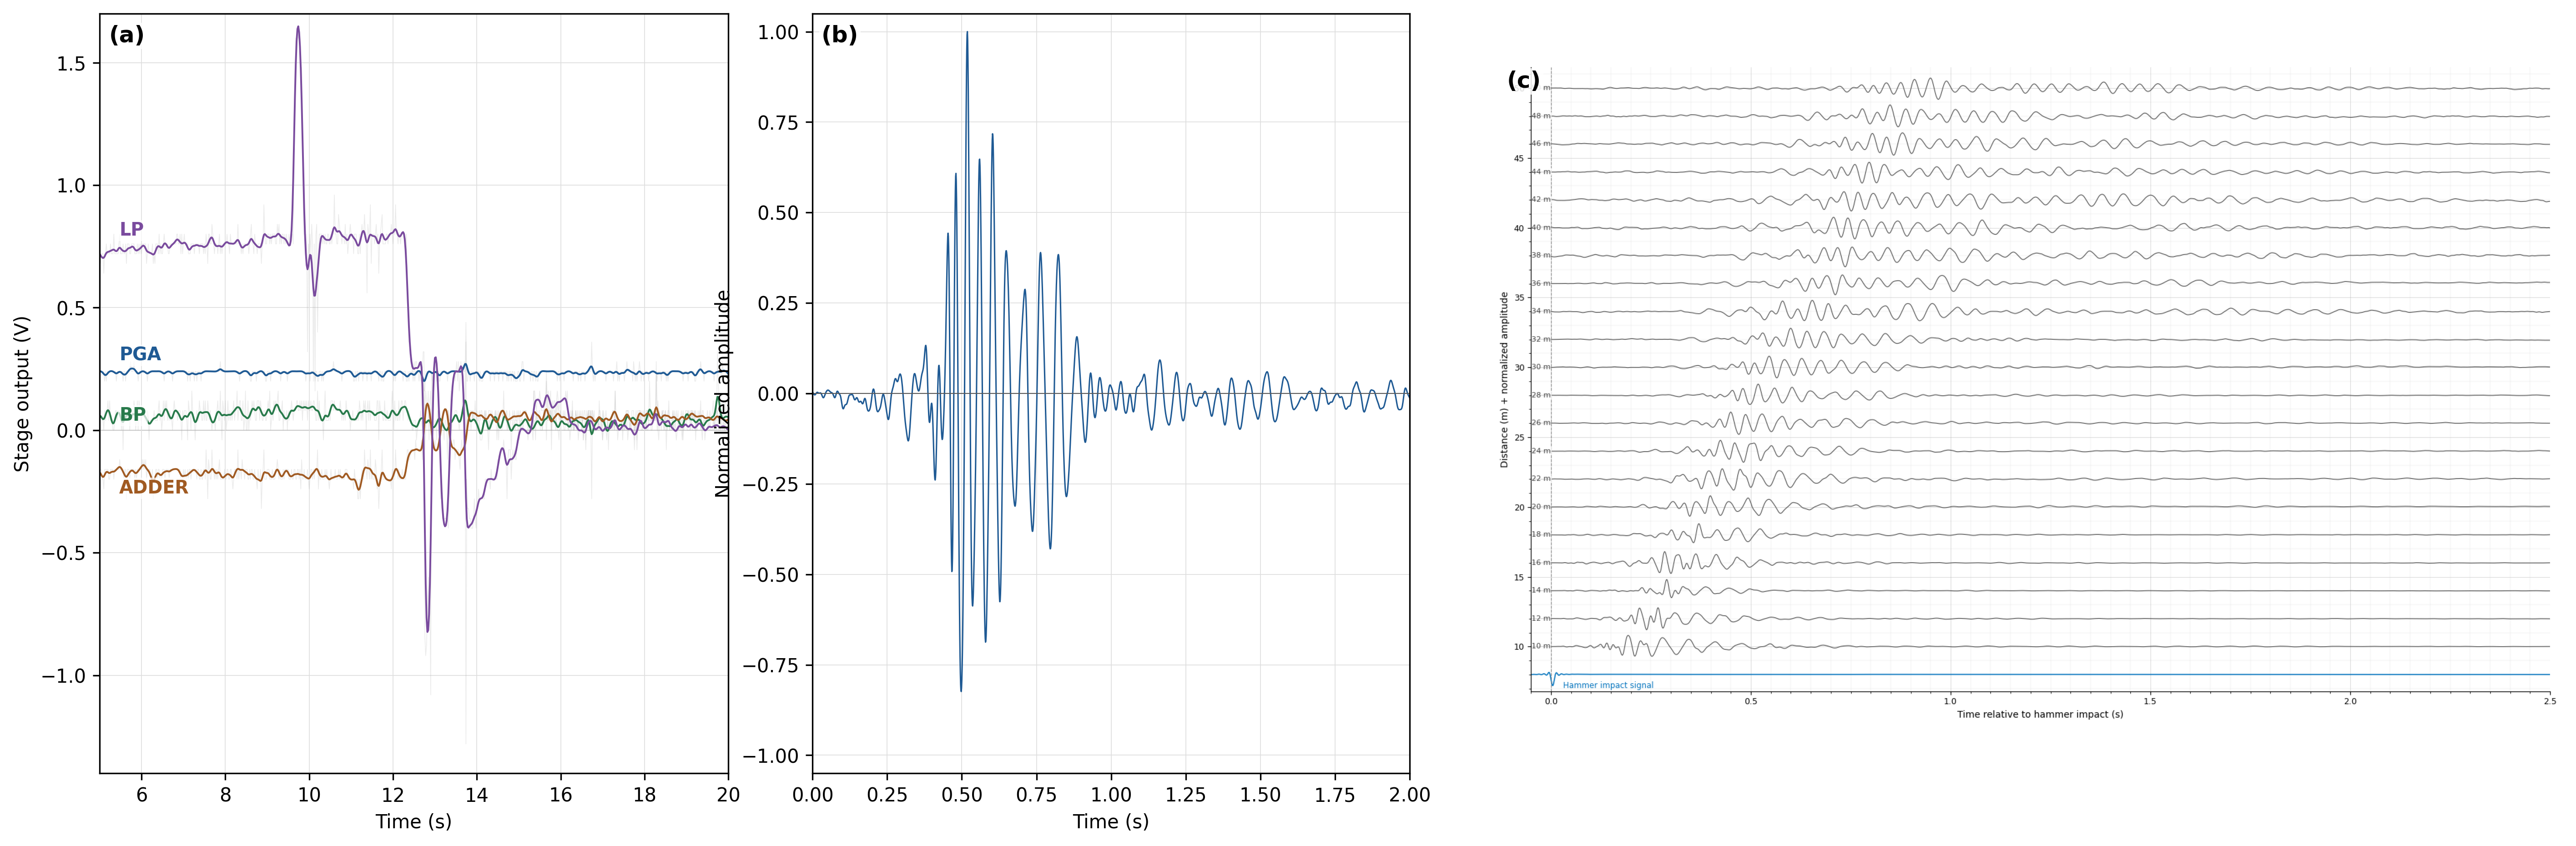
\includegraphics[width=\textwidth]{autocalibration_signal_waterfall_composite.png}
\caption{Evidencia visual integrada del tramo junio--julio: trayectoria de
auto-calibraci\'on, captura temporal y visualizaci\'on tipo \emph{waterfall}. El montaje
re\'une resultados de etapas distintas para mostrar la progresi\'on de banco a campo.}
\label{fig:cronologia-autocal-campo}
\end{figure}

Este per\'iodo produjo el aporte metodol\'ogico central del proyecto, y es un buen ejemplo
de iteraci\'on de dise\~no porque \textbf{el algoritmo se reemplaz\'o dos veces}.

La primera implementaci\'on us\'o \textbf{b\'usqueda binaria} (bisecci\'on) sobre los c\'odigos
VDAC, y se valid\'o en hardware real. Sobre esa base se realizaron dos avances
estructurales: la adquisici\'on migr\'o de una ISR cl\'asica a una \textbf{cadena gobernada
por DMA con filtro FIR embebido}, dejando al procesador fuera del camino de datos; y la
calibraci\'on gan\'o \textbf{persistencia en EEPROM con CRC-16}, sobreviviendo a un
reinicio. La cadena DMA se generaliz\'o luego a un multiplexor de cuatro canales
(crudo/filtrado $\times$ individual/lote) y se activ\'o el \textbf{promediado por
hardware}, de modo que la calibraci\'on dej\'o de promediar muestra a muestra en la
interrupci\'on y pas\'o a consumir ventanas ya sumadas, con verificaci\'on de coherencia en
tiempo de compilaci\'on.

El 23 de junio se produjo el \textbf{reemplazo total del algoritmo}. Tras convivir con
bisecci\'on binaria, un servo lento y variantes de control PID, el sistema converg\'io en
un \'unico
\textbf{controlador PI} con prealimentaci\'on f\'isica y detector de enganche, unificado
para ambos tipos de nodo, y se document\'o la primera calibraci\'on exitosa sobre hardware
real.

El refinamiento posterior aport\'o: escala del error en c\'odigos de DAC, banda muerta
proporcional a la ganancia de cada etapa, \textbf{anti-windup direccional} ---el
integrador se congela contra el l\'imite del DAC \'unicamente en el sentido que empeorar\'ia
la saturaci\'on--- y manejo correcto de ganancias con signo. El controlador se generaliz\'o
a las cuatro etapas de la placa de ge\'ofono y se elimin\'o definitivamente el c\'odigo de
bisecci\'on heredado.

Dos hallazgos de este per\'iodo merecen menci\'on por su valor pr\'actico. Primero, se
descubri\'o que el filtro de adquisici\'on llevaba \emph{meses} cargando coeficientes de
pasa-banda en lugar del pasa-bajos que correspond\'ia. Segundo, un problema que aparentaba
ser de firmware result\'o ser \textbf{un pin sin soldar}. El per\'iodo cierra corrigiendo
cuatro defectos de campo documentados y agregando detecci\'on autom\'atica del tipo de nodo,
propagada desde el PSoC hasta la interfaz web.

\subsection{Del 1 al 12 de julio --- Determinismo, almacenamiento y procesamiento MASW}

El modelo de captura pas\'o de estar gobernado por temporizador a basarse en
\textbf{confirmaci\'on real de fin de captura por nodo}, y la EEPROM de calibraci\'on se
redise\~n\'o para mantener \textbf{un registro independiente por c\'odigo de ganancia}.

El cambio de arquitectura m\'as importante fue el nacimiento de \textbf{\emph{superMaquina}}:
la l\'ogica de captura migr\'o de C a una m\'aquina de estados descrita en \textbf{Verilog} e
instanciada en los bloques UDB del PSoC, que decide en hardware qu\'e solicitud de DMA se
deja pasar y cu\'ando arranca y termina una captura. La motivaci\'on es el determinismo: en
un sistema multicanal el \emph{jitter} temporal se traduce directamente en error de
velocidad de fase. Se agreg\'o adem\'as un conjunto completo de comandos por USB para operar
el \emph{pipeline} paso a paso desde terminal, sin depender de la web.

Se consolid\'o la pol\'itica de eventos ``determinismo primero'': los eventos de fin de
cuenta de los temporizadores dejaron de generar interrupci\'on y pasaron a consumirse por
sondeo, se dedic\'o un temporizador al \emph{watchdog} de captura, y se agreg\'o un
\textbf{cortacircuitos anti-tormenta de interrupciones} ---una condici\'on efectivamente
observada en placa mediante depuraci\'on por pyOCD--- con auto-recuperaci\'on. El ADC pas\'o
de dos a \textbf{cuatro configuraciones de rango de entrada}, todas validadas en
hardware, y la interfaz web sum\'o indicador de intensidad de se\~nal del enlace.

En paralelo arranc\'o el \emph{pipeline} de procesamiento en Python, que sum\'o cerca de
\textbf{4600 l\'ineas} de una vez: m\'odulos de an\'alisis de dispersi\'on e inversi\'on MASW y
una aplicaci\'on de revisi\'on de datos de campo. Esta \'ultima recibi\'o doce fases de pulido
(ordenamiento por amplitud pico a pico, banco de filtros, alineaci\'on entre tandas,
\emph{waterfall} y $f$--$k$, selecci\'on de curvas) y luego la capacidad de definir grupos
de dispersi\'on independientes con combinaci\'on ponderada de im\'agenes, base de la
inversi\'on multimodal. Se integr\'o \texttt{maswavespy} como subm\'odulo y se corri\'o la
primera deconvoluci\'on sobre una captura real de campo.

El per\'iodo cierra con la \textbf{auditor\'ia pre-campo} descrita en detalle en la
Secci\'on~\ref{sec:auditoria}, que encontr\'o y corrigi\'o varios defectos cr\'iticos y emiti\'o
el veredicto de sistema listo para campo.

\subsection{Del 15 al 29 de julio --- Comunicaci\'on cient\'ifica y reorganizaci\'on}

Se redact\'o el art\'iculo sobre la auto-calibraci\'on para el congreso URUCON~2026,
incorporando datos experimentales reales de dos placas con barrido completo de ganancia.
El art\'iculo se someti\'o a un panel de revisi\'on editorial simulada y se respondi\'o a las
observaciones: siete referencias nuevas, tabla de resultados ampliada a las cuatro etapas
en lugar de solo la \'ultima, ecuaciones de banda muerta con justificaci\'on expl\'icita, y
una correcci\'on de honestidad cient\'ifica sobre qu\'e representa realmente la condici\'on de
referencia. Tras una reuni\'on con el tutor se comprimi\'o de seis a cinco p\'aginas.

En el firmware se salda una deuda de nomenclatura renombrando por completo la etapa
sumadora, y se hace configurable la banda muerta por etapa. En MATLAB se establece un
protocolo formal de barridos de la cadena anal\'ogica con \emph{script} de an\'alisis y
datos reales, que permiti\'o contrastar la respuesta medida contra el modelo del circuito
con valores de componentes reales.

Se produjo tambi\'en una \textbf{ruptura arquitect\'onica} del repositorio: el historial
monol\'itico se preserv\'o y el proyecto se reinici\'o como superproyecto con siete
subm\'odulos independientes, reorganizados poco despu\'es \textbf{por prop\'osito y no por
lenguaje} (firmware, interfaces, c\'alculos y modelados).

Finalmente se port\'o el servidor Python de una implementaci\'on artesanal a
\textbf{FastAPI}, con un \emph{gate} automatizado como condici\'on de avance, y se
migr\'o la aplicaci\'on de escritorio PyQt de revisi\'on de campo a la web hasta alcanzar
paridad funcional, incorporando cuarentena reversible en lugar de borrado f\'isico, cola
de trabajos de an\'alisis persistente, exportaciones reproducibles y un \emph{gate} de
\textbf{58 verificaciones}.

\subsection{1 de agosto --- Hacia el hardware definitivo y la fuente s\'ismica}

Se migr\'o el conexionado PSoC$\leftrightarrow$ESP32 a una \textbf{placa portadora
intermedia} con asignaci\'on de pines definitiva verificada por \emph{script}, primer paso
hacia una PCB propia. Este trabajo requiri\'o reconstruir por ingenier\'ia inversa los
valores de componentes del esquem\'atico anal\'ogico, dado que el archivo del dise\~no es un
binario propietario sin herramientas de lectura p\'ublicas; la reconstrucci\'on se realiz\'o
contrastando el binario con la asignaci\'on generada por el ajustador y las cabeceras de
pines, declarando expl\'icitamente el nivel de confianza de cada valor recuperado. El
resultado es que el dise\~no anal\'ogico dej\'o de estar atrapado en un formato cerrado.

En paralelo arranc\'o el dise\~no del \textbf{martillo de leva}, la fuente s\'ismica
repetible, atacado simult\'aneamente con un modelo anal\'itico 2D en Python y un modelo 3D
en Simscape Multibody derivado del CAD real. Ambos modelos detectaron errores propios ---
una interferencia axial entre la leva y el brazo, y una violaci\'on de conservaci\'on de
energ\'ia--- que est\'an pendientes de resoluci\'on.

\subsection{S\'intesis: caminos explorados y descartados}

Por su valor metodol\'ogico se listan expl\'icitamente las alternativas evaluadas y
abandonadas, con el motivo del descarte.

\begin{table}[h]
\centering\footnotesize
\caption{Alternativas de dise\~no evaluadas y descartadas durante el proyecto.}
\label{tab:descartes}
\begin{tabularx}{\textwidth}{@{}l X l@{}}
\toprule
\textbf{Alternativa} & \textbf{Motivo del descarte} & \textbf{Per\'iodo} \\
\midrule
Filtro pasivo RC de entrada & Reemplazado por FIR digital: tolerancias, deriva t\'ermica, fase no lineal y disponibilidad de DSP & abr. \\
Topolog\'ia Sallen-Key / VCVS & An\'alisis comparativo favorece MFB (comportamiento con ganancia y sensibilidad a componentes) & abr. \\
Topolog\'ia VCVS de la compensaci\'on & Sensibilidad a tolerancias frente a la MFB; la compensaci\'on anal\'ogica activa se mantuvo & abr.--may. \\
Filtro adaptativo LMS para \emph{notch} & Transitorio de convergencia y dependencia de la se\~nal; reemplazado por regresi\'on arm\'onica por lote & jun. \\
\emph{Notch} arm\'onico en el cliente web & Retardo de grupo y eliminaci\'on indiscriminada dentro de la banda MASW; el crudo se trata en post-proceso & jun. \\
Enlace SPI PSoC$\leftrightarrow$ESP32 & Migrado primero a UART; la versi\'on actual usa UART en bajada e I\textsuperscript{2}C en subida & may.--ago. \\
Calibraci\'on por bisecci\'on binaria & Reemplazada por PI unificado; no manejaba bien ruido ni signo de ganancia & jun. \\
Servo lento y variantes PID & Se descarta el t\'ermino derivativo: amplifica el ruido de medici\'on del ADC sin aportar en una planta cuasi-est\'atica; el controlador final es PI & jun. \\
Captura gobernada por temporizador & Reemplazada por confirmaci\'on real de fin por nodo & jul. \\
L\'ogica de captura en C sobre registro & Reemplazada por m\'aquina de estados en Verilog (determinismo) & jul. \\
Servidor HTTP artesanal & Migrado a FastAPI & jul. \\
Aplicaci\'on de escritorio PyQt & Portada a la web para unificar la interfaz de operador & jul. \\
Repositorio monol\'itico & Superproyecto con subm\'odulos organizados por prop\'osito & jul. \\
\bottomrule
\end{tabularx}
\end{table}

\nota{Esta secci\'on completa no entra en las 15 p\'aginas. Propuesta: para la entrega
formal reducirla a \emph{una p\'agina}, con un p\'arrafo por per\'iodo, m\'as la
Tabla~\ref{tab:descartes} (que es la que mejor muestra criterio de ingenier\'ia). El
texto \'integro se conserva para el libro de tesis de la Defensa Final.}

\section{Metodolog\'ia experimental y validaci\'on}
\label{sec:metodologia}

\subsection{Estrategia general de validaci\'on}

La validaci\'on del sistema se organiz\'o en cuatro niveles, de menor a mayor integraci\'on:

\begin{enumerate}[itemsep=0.15em]
    \item \textbf{Verificaci\'on de modelos} contra medici\'on de laboratorio (modelo del
    SM-24, modelo del amplificador operacional real, ganancias de continua de cada etapa).
    \item \textbf{Pruebas unitarias y de regresi\'on automatizadas} sobre el firmware y el
    software de procesamiento.
    \item \textbf{Caracterizaci\'on cuantitativa en banco} con instrumental de referencia
    (osciloscopio de cuatro canales) sobre m\'ultiples placas y configuraciones.
    \item \textbf{Pruebas de aceptaci\'on de sistema completo} (auditor\'ia pre-campo) y
    campa\~nas de medici\'on en campo.
\end{enumerate}

\subsection{Modelado y caracterizaci\'on del transductor}

El ge\'ofono SM-24 se model\'o en Simulink a partir de las ecuaciones de la
Secci\'on~\ref{sec:geo-tres-formas}, y el
modelo se contrast\'o con mediciones sobre el transductor real. Se desarrollaron
herramientas propias de an\'alisis:

\begin{itemize}[itemsep=0.15em]
    \item \texttt{geophone\_scope.m} y \texttt{geophone\_scope\_simple.m}: adquisici\'on y
    visualizaci\'on en tiempo real sobre puerto serie.
    \item \texttt{analisis\_espectral.m}: estimaci\'on de densidad espectral de potencia
    por el m\'etodo de Welch y c\'alculo de relaci\'on se\~nal--ruido por entidad de medici\'on.
    \item \texttt{ComparacionFiltros.m}: comparaci\'on cuantitativa de topolog\'ias de
    filtro, que fundament\'o la elecci\'on de MFB.
    \item Protocolo de barridos de la cadena anal\'ogica con \emph{script} de an\'alisis
    dedicado, que permiti\'o contrastar la respuesta medida contra el modelo del circuito
    con valores de componentes reales.
\end{itemize}

\begin{sloppypar}
Para hacer trazable el estado MASW mostrado en resultados, se fija el siguiente
\emph{snapshot}: \texttt{data} en el commit
{\ttfamily\footnotesize 76c4254b19cf\allowbreak c1f85edb9fb9\allowbreak
201b40c7f250\allowbreak b413},
software de procesamiento en
{\ttfamily\footnotesize 30b60517d337\allowbreak 7d175ecc7070\allowbreak
278c25cbca35\allowbreak b7ec}
y archivo
\nolinkurl{data/processed/Canchita/field_review_masw_state.json}, con SHA-256
{\ttfamily\footnotesize 8f8bf4d59a09\allowbreak 2b8f321b2829\allowbreak
af07fbfd3e03\allowbreak 374304c57310\allowbreak 3c39e1a43df3\allowbreak 0006}.
El estado guarda: imagen $c=\SIrange{50}{170}{\meter\per\second}$ con paso
\SI{0.1}{\meter\per\second} y $f=\SIrange{0.1}{35}{\hertz}$; grupo~1 con peso~1 y
grupo~2 con peso~0; 113 puntos etiquetados como modo~0; e inversi\'on de siete capas
m\'as semiespacio, 1000 iteraciones, $b_s=8$, $b_h=12$, $\nu=0{,}35$ y
$\rho=\SI{1850}{\kilogram\per\meter\cubed}$. El desajuste del \emph{port} se define como
\end{sloppypar}

\begin{equation}
E=\frac{100}{n}\sum_{i=1}^{n}\frac{|c_i^{\mathrm{obs}}-c_i^{\mathrm{teo}}|}
{c_i^{\mathrm{obs}}}\quad[\%].
\end{equation}

Este \emph{snapshot} permite repetir el estado num\'erico guardado, pero no reconstruye
por s\'i solo todas las decisiones manuales que llevaron al pol\'igono de selecci\'on. Esa
limitaci\'on es una raz\'on adicional para tratar la inversi\'on como exploratoria. La SNR
de la Fig.~\ref{fig:gather-main}, por su parte, se calcul\'o sobre la primera captura
v\'alida a \SI{1020}{\hertz} de cada posici\'on, no sobre una traza apilada: cociente entre
la desviaci\'on est\'andar posterior y previa al impacto, expresado como
$20\log_{10}(\sigma_{\mathrm{s}}/\sigma_{\mathrm{r}})$, donde los sub\'indices
$\mathrm{s}$ y $\mathrm{r}$ identifican las ventanas de se\~nal y ruido.

El modelo ideal no reprodujo el comportamiento medido del compensador en el extremo
superior de la banda. El primer modelo no ideal usado en los c\'alculos combin\'o
$A_0=\SI{90}{\decibel}$ con \SI{8}{\mega\hertz}, pero confundi\'o frecuencia de ganancia
unitaria con polo dominante. Esa parametrizaci\'on queda invalidada y debe recalcularse;
la funci\'on monopolo ya fue corregida en los scripts, pero la s\'intesis y la medici\'on
deben repetirse. El resultado anterior no se usa para sostener una banda compensada ya
demostrada.

\begin{figure}[ht]
\centering

\includegraphics[width=\textwidth]{barrido_crudo_cadena.png}
\caption{Ejemplo de barrido experimental conservado como evidencia de laboratorio:
se\~nales crudas de excitaci\'on y salida de la cadena antes de la estimaci\'on arm\'onica.
Los puntos medidos siguen siendo v\'alidos como registro; cualquier superposici\'on con
el modelo no ideal anterior debe recalcularse con el polo dominante corregido.}
\label{fig:barrido-crudo-metodo}
\end{figure}

\subsection{Validaci\'on experimental del DA-AFE}
\label{sec:met-daafe}

Este es el experimento m\'as riguroso realizado hasta la fecha y fue documentado en la
comunicaci\'on sometida a URUCON~2026; a\'un no se cuenta con dictamen externo.

\subsubsection{Dise\~no experimental}

Se evaluaron \textbf{ocho configuraciones placa--ganancia}: las cinco ganancias del PGA
sobre la Placa~A, m\'as las ganancias $\times16$, $\times32$ y $\times50$ sobre la
Placa~B. Cada configuraci\'on se evalu\'o mediante \textbf{diez reinicios apareados}
($N=10$).

Las decisiones metodol\'ogicas relevantes fueron:

\begin{itemize}[itemsep=0.15em]
    \item \textbf{Referencia com\'un}: se aplic\'o una \'unica l\'inea base de c\'odigos fijos,
    elegida emp\'iricamente sobre la Placa~B a $\times50$, \emph{sin} adaptarla a cada
    configuraci\'on. Esto es deliberadamente desfavorable a la l\'inea base: las reducciones
    reportadas acotan superiormente el beneficio respecto de un ajuste fijo por placa, en
    lugar de replicarlo.
    \item \textbf{Configuraci\'on \'unica de controlador}: los mismos par\'ametros de la
    Tabla~\ref{tab:cal_params} para todas las placas y ganancias, sin reajuste.
    \item \textbf{Medici\'on apareada}: dentro de cada reinicio se registr\'o siempre primero
    la condici\'on de referencia fija y luego la calibrada.
    \item \textbf{Escritura en EEPROM deshabilitada} tras la calibraci\'on, de modo que
    cada reinicio partiera exactamente de la misma l\'inea base.
    \item \textbf{Exclusiones declaradas}: la Placa~B a $\times1$ y $\times4$ se
    excluyeron porque sus residuos de l\'inea base ya ca\'ian dentro de las bandas muertas,
    impidiendo actualizaciones correctivas. El comportamiento esperado se confirm\'o con
    un diagn\'ostico separado de banda muerta m\'as estrecha.
\end{itemize}

\subsubsection{Procedimiento de medici\'on}

Un osciloscopio Tektronix TDS~2004B de cuatro canales registr\'o la tensi\'on media de
salida de las etapas PGA, BP, SUM y LP sobre una ventana de \SI{1}{\second} posterior al
establecimiento. Las masas de las puntas se conectaron a $V_{\mathrm{ref}}=V_{DDA}/2$,
de modo que cada canal midiera $V_{\mathrm{etapa}}-V_{\mathrm{ref}}$. La salida LP se
adopt\'o como m\'etrica principal por alimentar directamente al ADC.

\subsubsection{An\'alisis estad\'istico}

Se aplic\'o una \textbf{prueba de signos de una cola}~\cite{Conover1999} sobre las
mediciones apareadas de la etapa LP. La elecci\'on de una prueba no param\'etrica responde
al tama\~no de muestra y a no asumir normalidad de los residuos.

\subsection{Auditor\'ia pre-campo del sistema completo}
\label{sec:auditoria}

Antes de las campa\~nas de campo se ejecut\'o una auditor\'ia sistem\'atica sobre hardware
real, con una matriz de pruebas de aceptaci\'on identificadas E1--E18 que cubri\'o: capturas
en RAM y en SD de distinta duraci\'on, decimaci\'on y filtrado por radio, comandos de
captura a SD, verificaci\'on estricta por USB, interfaz en navegador, reconexi\'on de
WebSocket, detenci\'on en vivo, transiciones de rango y decimaci\'on, ciclo de apagado y
recuperaci\'on, y prueba de resistencia prolongada.

\subsubsection{Defectos cr\'iticos encontrados y corregidos}

La auditor\'ia detect\'o defectos que habr\'ian invalidado una campa\~na de campo. Se destacan
tres por su valor metodol\'ogico:

\begin{itemize}[itemsep=0.25em]
    \item \textbf{F1 --- Capturas largas destruidas por el \emph{watchdog}.} Un
    \emph{watchdog} de estancamiento de sincronizaci\'on re-disparaba el comando de arranque
    y destru\'ia las sesiones largas en SD. El s\'intoma observado era desconcertante: una
    captura de 10 minutos aceptada con \emph{cero muestras}. Se corrigi\'o con un margen
    proporcional y un aborto limpio.
    \item \textbf{F9 --- El arranque romp\'ia el nodo.} Defecto de carrera:
    el maestro esperaba la confirmaci\'on de armado con un tiempo l\'imite de
    \SI{120}{\milli\second}, pero la confirmaci\'on real de ``PSoC armado'' tarda
    \SI{130}{\milli\second}. El reintento reemit\'ia la secuencia completa de preparaci\'on,
    forzando un segundo comando de configuraci\'on; pero el PSoC, ya armado, entra en
    silencio total por dise\~no. El comando nunca se confirmaba, y el esclavo interpretaba
    el vencimiento como fallo y liberaba el almac\'en, mientras el PSoC segu\'ia f\'isicamente
    armado esperando un flanco de sincronismo que nadie volver\'ia a emitir. El nodo quedaba
    inutilizable hasta un reinicio f\'isico. Es un ejemplo did\'actico de c\'omo una carrera
    de \SI{10}{\milli\second} entre dos temporizadores produce una falla determinista y
    total. Se corrigi\'o en dos capas: el reintento dej\'o de reemitir la preparaci\'on, y el
    comando de preparaci\'on se hizo idempotente.
    \item \textbf{F5 --- Cliente colgado en conexi\'on semiabierta.} La herramienta de
    descarga no ten\'ia \emph{watchdog} de silencio y quedaba bloqueada sobre un
    \emph{socket} zombi.
\end{itemize}

\subsubsection{Criterio de aceptaci\'on}

La prueba de aceptaci\'on definitiva consisti\'o en una captura continua de 10 minutos con
verificaci\'on de integridad de extremo a extremo: conteo de lotes en SD, conteo de
muestras recibidas por radio, tama\~no en bytes, n\'umero de conexiones y desconexiones, y
recomputaci\'on de la suma SHA-256. La adopci\'on de un criterio de integridad
criptogr\'afica ---en lugar de una inspecci\'on visual de las se\~nales--- fue deliberada:
permite distinguir una transferencia completa de una truncada, distinci\'on que result\'o
decisiva, ya que un intento previo hab\'ia capturado correctamente en SD pero entregado un
archivo truncado por el lado del cliente.

\subsection{El sitio de ensayo: contexto geol\'ogico y verdad de terreno disponible}
\label{sec:sitio-sev}

Un elemento poco habitual en un trabajo de instrumentaci\'on, y que conviene explotar, es
que el sitio principal de medici\'on cuenta con una \textbf{caracterizaci\'on geof\'isica
independiente, previa y co-localizada}, realizada por terceros con un m\'etodo distinto.

En julio de 2023 la consultora V\'ictor Gonz\'alez \& Asoc.~S.S.\ ejecut\'o un estudio
hidrogeol\'ogico para la Facultad de Ciencias y Tecnolog\'ias de la UC, Campus Asunci\'on
--- Sede Santa Librada~\cite{GonzalezHidro2023}, sobre un \'area de proyecto de
\SI{0.186}{\kilo\meter\squared}. El estudio incluy\'o tres \textbf{Sondeos El\'ectricos
Verticales} (SEV) con arreglo Schlumberger, medidos con un resistiv\'imetro GOLD~DDC-8
(hasta \SI{700}{\volt} y \SI{3}{\ampere}, $AB/2$ m\'aximo \SI{500}{\meter}) e
interpretados con el programa IPI2win de la Universidad Estatal de Mosc\'u.

\textbf{El SEV~01 se ejecut\'o en la cancha de f\'utbol de la UC} (UTM
$X=\num{435595}$, $Y=\num{7198920}$), que es el mismo predio en el que se realizaron las
campa\~nas de adquisici\'on de este proyecto. Es, por lo tanto, una medici\'on
independiente del mismo subsuelo, con un m\'etodo geof\'isico completamente distinto
---resistividad el\'ectrica en corriente continua en lugar de ondas superficiales--- y
anterior al proyecto, de modo que no puede haber sido influida por \'el.

\subsubsection{Modelos geoel\'ectricos obtenidos}

\begin{table}[h]
\centering\footnotesize
\caption{Modelos de capas invertidos de los tres SEV~\cite{GonzalezHidro2023}.
$\rho$: resistividad; $h$: espesor; $d$: profundidad a la base. El SEV~01 es el
co-localizado con las campa\~nas de este proyecto.}
\label{tab:sev}
\begin{tabular}{@{}llrrrl@{}}
\toprule
Sondeo & Capa & $\rho$ [\si{\ohm\meter}] & $h$ [\si{\meter}] & $d$ [\si{\meter}] & Interpretaci\'on \\
\midrule
\multirow{6}{*}{\shortstack[l]{\textbf{SEV~01}\\ Cancha de f\'utbol\\ $AB/2=\SI{125}{\meter}$\\ cota \SI{72}{\meter} s.n.m.}}
 & 1 & 1186  & 1{,}00 & 1{,}00  & Suelo residual seco, muy compactado \\
 & 2 & 15    & 1{,}06 & 2{,}06  & Nivel conductivo delgado (arcilloso) \\
 & 3 & 105   & 2{,}09 & 4{,}15  & Sedimentos areno-cuarzosos \\
 & 4 & 24{,}2 & 19{,}9 & \textbf{24{,}0} & Cementaci\'on arcillosa; \textbf{base del suelo} \\
 & 5 & 126   & 47{,}7 & \textbf{71{,}8} & Acu\'ifero Cuaternario/Pati\~no \\
 & 6 & 6{,}42 & --- & --- & Areniscas con matriz arcillosa \\
\midrule
\multirow{4}{*}{\shortstack[l]{SEV~02\\ Lindero norte\\ $AB/2=\SI{125}{\meter}$}}
 & 1 & 220   & 1{,}00 & 1{,}00  & Suelo residual seco \\
 & 2 & 36{,}6 & 12{,}0 & 13{,}0 & Sedimentos con mayor arcilla \\
 & 3 & 95{,}8 & 9{,}73 & 22{,}7 & Nivel cuarzoso \\
 & 4 & 30{,}8 & --- & --- & Basal arcilloso \\
\midrule
\multirow{4}{*}{\shortstack[l]{SEV~03 (param\'etrico)\\ Junto al pozo FT01\\ $AB/2=\SI{80}{\meter}$}}
 & 1 & 202   & 1{,}02 & 1{,}02 & Suelo residual seco \\
 & 2 & 117   & 7{,}34 & 8{,}36 & Areno-cuarzoso resistivo \\
 & 3 & 54{,}4 & 56{,}1 & 64{,}5 & Acu\'ifero \\
 & 4 & 3{,}64 & --- & --- & Basal arcilloso \\
\bottomrule
\end{tabular}
\end{table}

El SEV~03 es \textbf{param\'etrico}: se midi\'o junto a un pozo tubular profundo existente
(FT01, \SI{50}{\meter} de profundidad, en operaci\'on, conductividad el\'ectrica
\SI{130}{\micro\siemens\per\centi\meter}, pH~7{,}1), de modo que su modelo est\'a anclado
a litolog\'ia conocida. Eso da trazabilidad a la interpretaci\'on de los otros dos.

\subsubsection{Qu\'e aporta esto al proyecto}

\paragraph{a) Contrastes esperables en el perfil $V_S$.} El SEV~01 sit\'ua la
\textbf{base del suelo en \SI{24.0}{\meter}} y la base de la secuencia media en
\SI{71.8}{\meter}. Debe subrayarse una salvedad metodol\'ogica: \textbf{un contraste de
resistividad no es un contraste de rigidez}. La resistividad responde a porosidad,
salinidad del fluido y contenido de arcilla; $V_S$ responde a la rigidez al corte del
esqueleto. Coinciden a menudo, porque ambos siguen los cambios litol\'ogicos, pero no por
construcci\'on. Por eso las profundidades de la Tabla~\ref{tab:sev} se enuncian aqu\'i como
\emph{contrastes esperables} contra los cuales contrastar el perfil invertido, y no como
una predicci\'on que el MASW deba reproducir. Aun as\'i, el valor de la comparaci\'on es
alto: una interfaz a \SI{24}{\meter} cae de lleno dentro del objetivo de
\SI{50}{\meter} del proyecto, y es exactamente el tipo de rasgo que un perfil $V_S$
correctamente invertido deber\'ia resolver.

\paragraph{b) El nivel fre\'atico, con un n\'umero concreto.} El estudio ubica el nivel
del agua \textbf{entre \SI{10}{} y \SI{30}{\meter} de profundidad}, con la aclaraci\'on
expresa de que la campa\~na se realiz\'o en \'epoca de escasas precipitaciones, de modo
que se trata de una cota de estiaje y no del r\'egimen anual. Esto cierra un cabo suelto
del \S\ref{sec:no-unicidad}: all\'i se se\~nala que ignorar el nivel fre\'atico equivale a
asumir una raz\'on de Poisson incorrecta en las capas saturadas, donde el comportamiento
no drenado lleva $\nu\to0{,}5$. Ahora existe un rango concreto y con fuente para
parametrizar esa transici\'on en la inversi\'on ---y, m\'as importante, la advertencia de
que su profundidad es \textbf{estacional}, por lo que la fecha de cada campa\~na de este
proyecto es un dato relevante y no un detalle administrativo.

\paragraph{c) Marco litol\'ogico.} El sitio se asienta sobre el \textbf{Grupo Asunci\'on}
(Cret\'acico), relleno de una fosa tect\'onica tipo semi-graben: la Formaci\'on Pati\~no
en la base (fanglomerados, del orden de \SI{100}{\meter} de espesor) y la Formaci\'on
Yaguar\'on por encima (areniscas cuarzosas de grano fino a medio, friables, con matriz
arcillosa), que constituye el nivel productor del \textbf{Acu\'ifero Pati\~no}. Se trata
de sedimentos cl\'asticos poco cementados: es decir, exactamente el r\'egimen de suelo
blando a intermedio para el cual se asumieron velocidades de onda Rayleigh
$V_R\approx\SIrange{150}{250}{\meter\per\second}$ al derivar la banda objetivo en la
Ec.~\eqref{eq:geo-banda-objetivo}. La hip\'otesis que sostiene el requisito de banda del
proyecto queda as\'i respaldada por la geolog\'ia documentada del sitio y no s\'olo por un
valor de manual.

\paragraph{d) Un paralelo instructivo sobre la limitaci\'on de apertura.} El propio
estudio declara que la exploraci\'on qued\'o limitada a \SI{125}{\meter} de profundidad
``por limitaciones de espacio en \'area eminentemente urbana''. Es la misma clase de
restricci\'on ---no instrumental sino de sitio--- que limita la apertura del arreglo de
este proyecto, y vale citarla porque muestra que el problema no es exclusivo de un
prototipo de bajo costo: un equipo comercial operado por especialistas enfrent\'o la
misma barrera en el mismo predio.

\paragraph{e) Contraste con el criterio de Comina.} La geometr\'ia efectivamente
desplegada (apertura $L=\SI{40}{\meter}$, v\'ease m\'as abajo) admite longitudes de onda
resueltas del orden de la propia apertura. Frente al criterio
$\lambda_{\max}>\SI{60}{\meter}$ de Comina \emph{et al.}~\cite{Comina2011}
(\S\ref{sec:buenas-practicas}), \textbf{la apertura actual es insuficiente} para el
r\'egimen en que la no unicidad deja de dominar el error de $V_{S,30}$. Esto identifica
con precisi\'on el pr\'oximo cuello de botella del proyecto: \emph{no es la electr\'onica,
es la longitud del tendido}. Ampliar la apertura no requiere diseño nuevo, requiere m\'as
nodos ---que es justamente lo que la arquitectura inal\'ambrica fue pensada para
permitir.

\paragraph{f) Una validaci\'on invasiva al alcance de la mano.} El estudio
\textbf{recomienda perforar un pozo de \SI{60}{\meter} exactamente en el sector del
SEV~01}, es decir en la cancha, con perfilaje geof\'isico de pozo (resistividad, potencial
espont\'aneo y gamma natural). Si esa perforaci\'on llega a ejecutarse, el proyecto
tendr\'ia una \textbf{referencia invasiva directa en el mismo punto donde midi\'o},
reproduciendo a escala de un sitio el experimento de la segunda parte de
InterPACIFIC~\cite{Garofalo2016b}: contrastar un m\'etodo no invasivo contra perforaci\'on.
Es el mejor escenario de validaci\'on que este trabajo podr\'ia aspirar a tener y se
registra como l\'inea futura prioritaria (\S\ref{sec:futuros}).

\nota{Falta confirmar que las coordenadas registradas en los metadatos de las capturas de
``Canchita'' caen efectivamente dentro del entorno del SEV~01 (UTM 435595 / 7198920).
La identificaci\'on por nombre de sector (``cancha de f\'utbol de la UC'') es inequ\'ivoca,
pero conviene dejar asentada la distancia real entre el centro del tendido y el punto del
SEV, porque de ella depende cu\'an literal puede ser la comparaci\'on.}

\subsection{Campa\~nas de medici\'on en campo}

Se realizaron campa\~nas de adquisici\'on en varios sitios, con conjuntos de datos crudos
catalogados y versionados con Git~LFS y deduplicaci\'on por SHA-256. El cat\'alogo registra
del orden de \textbf{22\,000 archivos crudos} (aproximadamente \SI{28}{\gibi\byte})
distribuidos en tres sitios de medici\'on, m\'as los conjuntos procesados
correspondientes.

La geometr\'ia efectivamente usada fue un \textbf{arreglo virtual o apertura sint\'etica},
no un tendido f\'isico simult\'aneo de 21 ge\'ofonos. El martillo permaneci\'o en
$x=\SI{0}{\meter}$ y un ge\'ofono se desplaz\'o en incrementos de
$\Delta x=\SI{2}{\meter}$; cada registro contiene dos roles
(\texttt{n\_slaves=2}): martillo y ge\'ofono. El \emph{gather} se reconstruye alineando
capturas de impactos distintos mediante el canal de martillo.

Esta econom\'ia de hardware introduce una hip\'otesis adicional respecto del MASW
multicanal simult\'aneo: la fuente y el acoplamiento deben ser suficientemente repetibles,
y las condiciones del sitio deben permanecer estacionarias mientras se mueve el receptor.
Se registraron m\'ultiples repeticiones por posici\'on para apilar y evaluar esa
repetibilidad. En el conjunto procesado vigente, el grupo~1 cubre
$x=\SIrange{10}{50}{\meter}$ con 21 posiciones y apertura
$L=\SI{40}{\meter}$; el grupo~2 cubre $x=\SIrange{10}{36}{\meter}$ con 14 posiciones y
$L=\SI{26}{\meter}$.

\begin{figure}[ht]
\centering

\includegraphics[width=\textwidth]{captura_cruda_campo.png}
\caption{Registro crudo real usado para ilustrar el procedimiento de campo
($x=\SI{24}{\meter}$): canal de martillo, ge\'ofono con su nivel de continua y salida
FIR. La marca temporal proviene del impacto; una traza individual no demuestra
repetibilidad entre golpes ni coherencia equivalente a un arreglo simult\'aneo.}
\label{fig:captura-cruda-metodo}
\end{figure}

\subsection{Procesamiento de los registros de campo}

El tratamiento de los registros incorpor\'o varias correcciones sistem\'aticas que
surgieron de la propia pr\'actica:

\begin{itemize}[itemsep=0.15em]
    \item \textbf{Polaridad}: se estableci\'o una convenci\'on fija (ge\'ofono no invertido,
    martillo invertido) y se implement\'o correcci\'on de polaridad por punto de medici\'on,
    autom\'atica y manual, dado que un error de signo en un canal corrompe la imagen de
    dispersi\'on.
    \item \textbf{Alineaci\'on entre tandas (\emph{enfase})}: aplicada por carpeta de
    medici\'on, con una etapa de limpieza de desplazamientos por se\~nal.
    \item \textbf{Mezcla de frecuencias de muestreo}: los registros tomados a
    \SI{2929}{\hertz} y a \SI{1020}{\hertz} se combinan mediante remuestreo racional.
    \item \textbf{Deduplicaci\'on por captura} y \textbf{rechazo expl\'icito de carpetas}
    defectuosas, que las excluye de los promedios sin alterar su validez individual.
\end{itemize}

\begin{figure}[ht]
\centering

\includegraphics[width=\textwidth]{preprocesamiento_espectral.png}
\caption{Ejemplo de preprocesamiento de un barrido: ventana temporal, espectro y
estimaci\'on de la componente arm\'onica. Esta separaci\'on entre dato crudo y estimador es
la base de las curvas de respuesta experimentales.}
\label{fig:preprocesamiento-espectral}
\end{figure}

\nota{Para la versi\'on de 15 p\'aginas: conservar \S5.3 completo (es el experimento
publicable) y \S5.4.1 resumido a los defectos F1 y F9 en un p\'arrafo. \S5.2, \S5.5 y
\S5.6 pueden comprimirse fuertemente. La geometr\'ia debe conservarse: sin ella no se
puede interpretar la profundidad alcanzable ni la naturaleza virtual del arreglo.}

\section{Resultados}
\label{sec:resultados}

\subsection{Validaci\'on experimental del DA-AFE}

El resultado cuantitativo m\'as s\'olido obtenido hasta la fecha corresponde a la
validaci\'on de la auto-calibraci\'on del \emph{front-end} anal\'ogico, cuyo dise\~no
experimental se describe en la Secci\'on~\ref{sec:met-daafe}.

La Tabla~\ref{tab:results} presenta la media y la desviaci\'on est\'andar muestral del
\emph{offset} residual normalizado sobre diez reinicios apareados. Cada columna es una
configuraci\'on placa--ganancia y cada fila una etapa anal\'ogica en orden de calibraci\'on;
en cada celda, el valor superior corresponde a la referencia fija compartida y el
inferior a la condici\'on calibrada. Leer una columna de arriba hacia abajo muestra c\'omo
el \emph{offset} se reduce etapa por etapa.

\begin{table}[h]
\centering
\scriptsize
\setlength{\tabcolsep}{3.0pt}
\caption{\emph{Offset} de continua residual (\% del fondo de escala del rango nominal de
\SI{5}{\volt} del ADC), media $\pm$ desviaci\'on est\'andar muestral sobre $N=10$ reinicios
apareados. En cada celda: arriba, referencia fija compartida; abajo, condici\'on
calibrada. Menor es mejor.}
\label{tab:results}
\begin{tabular}{lcccccccc}
\toprule
Etapa & A,\,$\times1$ & A,\,$\times4$ & A,\,$\times16$ & A,\,$\times32$ & A,\,$\times50$ & B,\,$\times16$ & B,\,$\times32$ & B,\,$\times50$\\
\midrule
\multirow{2}{*}{PGA}
 & $3{,}5\pm0{,}2$ & $2{,}4\pm0{,}1$ & $2{,}4\pm0{,}1$ & $1{,}0\pm0{,}2$ & $1{,}2\pm0{,}3$ & $2{,}1\pm0{,}1$ & $1{,}0\pm0{,}2$ & $2{,}5\pm0{,}1$\\
 & $3{,}4\pm0{,}3$ & $2{,}1\pm0{,}3$ & $1{,}9\pm0{,}2$ & $0{,}5\pm0{,}2$ & $1{,}0\pm0{,}5$ & $1{,}7\pm0{,}1$ & $0{,}5\pm0{,}2$ & $1{,}8\pm0{,}3$\\
\addlinespace[2pt]
\multirow{2}{*}{BP}
 & $1{,}5\pm2{,}2$ & $4{,}9\pm0{,}3$ & $3{,}8\pm0{,}9$ & $7{,}0\pm0{,}4$ & $1{,}0\pm0{,}7$ & $0{,}66\pm0{,}02$ & $0{,}66\pm0{,}01$ & $0{,}65\pm0{,}01$\\
 & $1{,}2\pm0{,}2$ & $1{,}0\pm0{,}2$ & $1{,}5\pm1{,}5$ & $1{,}0\pm0{,}5$ & $0{,}9\pm0{,}5$ & $0{,}66\pm0{,}02$ & $0{,}66\pm0{,}01$ & $0{,}65\pm0{,}02$\\
\addlinespace[2pt]
\multirow{2}{*}{SUM}
 & $\mathbf{21{,}8\pm1{,}1}^{\dagger}$ & $6{,}7\pm1{,}0$ & $4{,}9\pm1{,}5$ & $7{,}4\pm0{,}3$ & $0{,}4\pm0{,}2$ & $4{,}5\pm0{,}8$ & $8{,}0\pm0{,}8$ & $0{,}9\pm0{,}6$\\
 & $0{,}8\pm0{,}2$ & $1{,}0\pm0{,}3$ & $1{,}4\pm1{,}5$ & $0{,}6\pm0{,}2$ & $\mathbf{0{,}8\pm0{,}6}^{\ddagger}$ & $0{,}6\pm0{,}5$ & $1{,}2\pm0{,}3$ & $0{,}9\pm0{,}6$\\
\addlinespace[2pt]
\multirow{2}{*}{LP}
 & $\mathbf{45{,}8\pm3{,}1}^{\dagger}$ & $\mathbf{42{,}6\pm4{,}2}^{\dagger}$ & $\mathbf{29{,}6\pm6{,}8}^{\dagger}$ & $\mathbf{12{,}4\pm1{,}3}^{\dagger}$ & $4{,}1\pm2{,}1$ & $3{,}0\pm0{,}1$ & $2{,}9\pm0{,}1$ & $2{,}9\pm0{,}1$\\
 & $3{,}2\pm0{,}9$ & $3{,}9\pm0{,}8$ & $2{,}3\pm1{,}4$ & $1{,}7\pm0{,}7$ & $1{,}2\pm0{,}4$ & $0{,}7\pm0{,}1$ & $0{,}4\pm0{,}2$ & $0{,}7\pm0{,}2$\\
\bottomrule
\end{tabular}

\vspace{2pt}
\footnotesize
$^{\dagger}$Referencia fija $\geq\SI{10}{\percent}$ del fondo de escala.\quad
$^{\ddagger}$\'Unica media calibrada superior a su l\'inea base.
\end{table}

\subsubsection{S\'intesis de los resultados}

\begin{itemize}[itemsep=0.2em]
    \item En las ocho configuraciones evaluadas, el \emph{offset} residual a la salida LP
    ---la que alimenta directamente al ADC--- se redujo de
    \SIrange{2.9}{45.8}{\percent} a \SIrange{0.4}{3.9}{\percent} del fondo de escala.
    Las observaciones individuales calibradas se ubicaron entre
    \SIrange{0.1}{5.2}{\percent}.
    \item Una \textbf{prueba de signos de una cola}~\cite{Conover1999} sobre las
    mediciones apareadas de la etapa LP rechaz\'o la hip\'otesis nula de ausencia de
    reducci\'on en \textbf{las ocho configuraciones} (10 de 10 reinicios apareados, con
    $p\approx10^{-3}$ exacto), resultado que sobrevive a la correcci\'on de Bonferroni
    por comparaciones m\'ultiples.
    \item El resultado se obtuvo con una \textbf{\'unica configuraci\'on de controlador}
    para todas las placas y ganancias, sin reajuste espec\'ifico por placa ni por
    ganancia, lo que respalda la robustez del m\'etodo.
    \item Las etapas cuyo residuo de l\'inea base ya se ubica dentro de su banda muerta
    quedan sin modificar por dise\~no, comportamiento visible en la fila BP de la Placa~B.
\end{itemize}

\subsubsection{Temporizaci\'on}

La correcci\'on visible en las trayectorias de calibraci\'on abarca aproximadamente
\SI{7}{\second}, y las observaciones informales de banco indicaron completitud en torno
a los \SI{10}{\second}. Las ventanas de tiempo l\'imite configuradas totalizan
\SI{57.6}{\second} (aproximadamente \SI{60.5}{\second} incluyendo establecimiento y
refinamiento), excluyendo la sobrecarga de conmutaci\'on. Cuando existe una calibraci\'on
almacenada v\'alida s\'olo se ejecutan los intervalos de establecimiento por etapa
(2560 muestras, alrededor de \SI{1.0}{\second} a \SI{2604}{\hertz}, tasa vigente en esa campa\~na).

No se registraron vencimientos de tiempo l\'imite durante los experimentos reportados. El
\'unico observado en banco correspondi\'o a una placa alimentada mientras su ge\'ofono estaba
en movimiento, cuyo transitorio de alterna viola la hip\'otesis cuasi-est\'atica requerida
por la calibraci\'on \emph{foreground}.

\subsubsection{Limitaciones declaradas}

Por transparencia se explicitan las limitaciones del experimento, tal como fueron
reportadas en la comunicaci\'on cient\'ifica:

\begin{itemize}[itemsep=0.15em]
    \item El estudio se limit\'o a \textbf{dos placas ensambladas independientemente} y a
    un orden de calibraci\'on fijo; no establece desempe\~no estad\'istico poblacional.
    \item No se caracteriz\'o la \textbf{deriva de largo plazo} ni el apareamiento entre
    canales a lo largo de un arreglo completo.
    \item La evidencia concierne al \textbf{punto de operaci\'on} de la cadena de
    acondicionamiento, no al desempe\~no s\'ismico de extremo a extremo.
    \item La mejora relativamente modesta en la etapa PGA refleja el criterio de parada
    seleccionado (banda muerta amplia por tener $|K_{\mathrm{PGA}}|=1$) y no
    inestabilidad del controlador. Un diagn\'ostico separado con banda muerta m\'as estrecha
    redujo el residuo LP de \SI{2.98}{\percent} a \SI{0.84}{\percent}, indicando que hay
    margen de mejora por optimizaci\'on de par\'ametros.
\end{itemize}

No obstante, un \emph{offset} de referencia fija como el \SI{21.8}{\percent} medido a la
salida de la etapa sumadora ya consume m\'as de la quinta parte del rango de entrada del
amplificador y del ADC antes de aplicar se\~nal s\'ismica alguna, lo que dimensiona la
relevancia pr\'actica de la correcci\'on.

\subsection{Validaci\'on funcional del sistema de adquisici\'on}

\begin{itemize}[itemsep=0.2em]
    \item \textbf{Auditor\'ia pre-campo}: la matriz de pruebas de aceptaci\'on E1--E18 se
    complet\'o con resultado satisfactorio en todos sus \'items, tras la correcci\'on de los
    defectos cr\'iticos descritos en la Secci\'on~\ref{sec:auditoria}.
    \item \textbf{Captura continua de 10 minutos}: 52\,080 lotes escritos en SD sobre
    52\,080 esperados, 1\,562\,400 muestras transferidas por radio sobre 1\,562\,400
    esperadas, 4\,687\,200 bytes, una \'unica conexi\'on, cero desconexiones y suma
    SHA-256 recomputada coincidente.
    \item \textbf{Regresi\'on por USB}: 33 de 33 verificaciones satisfactorias, cubriendo
    modos crudo y filtrado, escritura y lectura de SD, confirmaciones de comando y
    restauraci\'on de estado.
    \item \textbf{Repetibilidad de extremo a extremo}: 10 de 10 ciclos completos
    satisfactorios, con integridad verificada en cada uno.
    \item \textbf{Robustez de comunicaci\'on}: corte de WebSocket inyectado durante la
    descarga con recuperaci\'on correcta y transferencia completada; detenci\'on en vivo
    validada tanto durante la captura como durante la descarga.
    \item \textbf{Transiciones de configuraci\'on}: 49 de 49 transiciones de rango de ADC
    y factor de decimaci\'on satisfactorias; 30 de 30 ciclos de apagado y recuperaci\'on.
    \item \textbf{Software de procesamiento}: \emph{gate} automatizado de 58
    verificaciones satisfactorio como condici\'on de avance del porteo web.
\end{itemize}

\subsection{Adquisici\'on en campo y procesamiento MASW}

Se realizaron campa\~nas de medici\'on en tres sitios (con dos campa\~nas separadas en uno
de ellos), cuyos conjuntos de datos crudos
est\'an catalogados y versionados con deduplicaci\'on por suma criptogr\'afica. El cat\'alogo
registra del orden de \textbf{22\,000 archivos crudos} (aproximadamente
\SI{28}{\gibi\byte}) junto con los conjuntos procesados correspondientes.

Sobre esos registros el \emph{pipeline} produce:

\begin{itemize}[itemsep=0.15em]
    \item Registros multicanal coherentes visualizables en formato \emph{waterfall} y de
    trazas, con correcci\'on de polaridad y alineaci\'on entre tandas.
    \item Im\'agenes de dispersi\'on en el dominio frecuencia--velocidad de fase, con
    combinaci\'on ponderada de m\'ultiples disparos.
    \item Curvas de dispersi\'on extra\'idas por modo mediante regiones-pol\'igono, editables
    antes de la inversi\'on.
    \item Perfiles $V_S(z)$ obtenidos por inversi\'on multimodal.
\end{itemize}

\nota{\textbf{Pendiente importante a conversar.} Los perfiles $V_S$ obtenidos a\'un no
est\'an contrastados contra un ensayo de referencia (SPT o similar), por lo que en este
documento se reportan como resultado del \emph{pipeline} y no como caracterizaci\'on
geot\'ecnica validada del sitio. Hay que decidir si conviene: (a) presentar un perfil
$V_S$ concreto ya en la Primera Presentaci\'on aclarando expl\'icitamente que la validaci\'on
externa est\'a pendiente, o (b) reportar \'unicamente la capacidad del \emph{pipeline} y
dejar los perfiles para la Defensa Final. Mi sugerencia es (a) con la aclaraci\'on, porque
demuestra que la cadena completa cierra.}

\nota{Faltan por incorporar a este documento las \textbf{figuras}: cadena anal\'ogica,
diagrama de hardware digital, trayectorias de calibraci\'on, \emph{waterfall} de campo e
imagen de dispersi\'on. Todas existen ya en \texttt{docs/Urucom\_2026\_compact/imagenes/}
y en las salidas del \emph{pipeline}; falta elegir cu\'ales entran seg\'un el recorte que
definamos.}

\section{Trabajos futuros}
\label{sec:futuros}

Los trabajos pendientes se agrupan en cinco frentes, ordenados aproximadamente por
prioridad y por dependencia mutua.

\subsection{Consolidaci\'on del hardware: de placas de desarrollo a PCB propia}

El sistema opera hoy sobre placas de desarrollo (CY8CKIT-059 y ESP32~DevKitC) cableadas
entre s\'i. El 1 de agosto se dio el primer paso de la migraci\'on al adoptar una
\textbf{placa portadora intermedia} con asignaci\'on de pines definitiva y verificada
autom\'aticamente. Los pasos restantes son:

\begin{itemize}[itemsep=0.15em]
    \item Trasladar el dise\~no anal\'ogico completo a \textbf{KiCad}, aprovechando que los
    valores de componentes ya fueron recuperados del formato binario propietario y
    documentados con su nivel de confianza.
    \item Dise\~nar, fabricar y ensamblar la PCB del nodo ge\'ofono, integrando PSoC, ESP32,
    alimentaci\'on, conector de ge\'ofono y ranura de tarjeta SD.
    \item Resolver la alimentaci\'on aut\'onoma del nodo: dimensionamiento de bater\'ia,
    regulaci\'on de bajo ruido y estimaci\'on de autonom\'ia para una jornada de campo.
    \item Dise\~nar el encapsulado y el sistema de acople al terreno.
\end{itemize}

\subsection{Fuente s\'ismica repetible: el martillo de leva}

La calidad de la imagen de dispersi\'on depende directamente de la repetibilidad de la
fuente, y una maza operada manualmente introduce variabilidad en energ\'ia, punto de
impacto y verticalidad. Wood y Cox~\cite{Wood2012} cuantificaron el efecto del tipo de
fuente sobre el sesgo y la incertidumbre de la curva de dispersi\'on, lo que justifica el
esfuerzo de mecanizar el impacto.

El dise\~no del \textbf{martillo de leva} arranc\'o el 1 de agosto con dos modelos
paralelos: uno anal\'itico bidimensional en Python y uno tridimensional en Simscape
Multibody derivado del CAD. Ambos detectaron errores propios que est\'an pendientes de
resoluci\'on: una \textbf{interferencia axial entre la leva y el brazo} (que invalida los
resultados de la simulaci\'on 3D en su estado actual) y una \textbf{violaci\'on de la
conservaci\'on de energ\'ia} en el modelo 2D. Las tareas siguientes son corregir ambos
modelos, converger a un perfil de leva, construir el mecanismo y caracterizar
experimentalmente la repetibilidad de la energ\'ia entregada y del instante de impacto.

\subsection{Conectividad y flujo de datos en campo}

El flujo actual requiere que un navegador est\'e escuchando en el momento de la captura,
porque el maestro no persiste los datos: \'estos se espejan en vivo por WebSocket y el
navegador los acumula. Adem\'as, mientras el tel\'efono est\'a conectado al punto de acceso
del maestro, el sistema operativo m\'ovil tiende a cortar o despriorizar los datos
m\'oviles al no detectar salida a internet, lo que bloquea cualquier sincronizaci\'on
autom\'atica.

Est\'a dise\~nado y con firmware implementado ---aunque a\'un sin probar en hardware--- un
\textbf{modo ENLACE} del maestro que resuelve ambos problemas permiti\'endole asociarse a
una red con salida a internet mientras mantiene su punto de acceso. Quedan pendientes:

\begin{itemize}[itemsep=0.15em]
    \item Probar el modo ENLACE en hardware y verificar que los esclavos adopten
    correctamente el canal del maestro cuando \'este cambia al asociarse a un router.
    \item Corregir un bloqueo mutuo detectado en el escaneo de redes cuando existe un
    identificador de red guardado que no est\'a presente.
    \item Implementar el servidor de datos del lado del anfitri\'on para persistencia
    autom\'atica, eliminando la dependencia de un navegador activo durante la captura.
\end{itemize}

\subsection{Ampliaci\'on del arreglo y campa\~na de validaci\'on}

\begin{itemize}[itemsep=0.15em]
    \item Escalar el arreglo desde la configuraci\'on actual hasta el n\'umero de canales
    objetivo, y caracterizar experimentalmente el \textbf{apareamiento entre canales} y
    el \emph{jitter} de sincronizaci\'on real sobre el arreglo completo ---magnitud que
    hasta ahora s\'olo se acot\'o por presupuesto te\'orico y por medici\'on sobre pocos nodos.
    \item Implementar y ensayar las \textbf{configuraciones matriciales} de medici\'on
    previstas en la propuesta, m\'as all\'a del arreglo lineal.
    \item Ejecutar una campa\~na de medici\'on en un sitio con \textbf{informaci\'on
    geot\'ecnica de referencia disponible} (SPT o equivalente).
    \item \textbf{Contrastar cuantitativamente} los perfiles $V_S$ obtenidos por MASW
    contra esa referencia. Este es el criterio de \'exito \'ultimo del proyecto y la
    validaci\'on que a\'un no se realiz\'o.
\end{itemize}

\subsection{Caracterizaci\'on complementaria de la instrumentaci\'on}

\begin{itemize}[itemsep=0.15em]
    \item \textbf{Validaci\'on estad\'istica sobre m\'as unidades}: el estudio del DA-AFE se
    limit\'o a dos placas; extenderlo a una poblaci\'on mayor permitir\'ia afirmaciones a
    nivel poblacional.
    \item \textbf{Deriva de largo plazo y comportamiento t\'ermico}: caracterizar la
    estabilidad de la calibraci\'on a lo largo de una jornada de campo y frente a
    variaciones de temperatura, no evaluadas hasta ahora.
    \item \textbf{Optimizaci\'on de par\'ametros del controlador}: el diagn\'ostico con banda
    muerta m\'as estrecha mostr\'o margen de mejora; una resoluci\'on de ajuste m\'as fina
    podr\'ia lograrse con DAC de salida de corriente o topolog\'ias de inyecci\'on con
    amortiguador, sin modificar el m\'etodo de calibraci\'on.
    \item \textbf{Extensi\'on del DA-AFE a otras funciones}: la calibraci\'on de
    \emph{offset} de continua es una demostraci\'on de factibilidad; el mismo principio de
    asistencia digital no intrusiva puede aplicarse a otras tareas de calibraci\'on y
    optimizaci\'on anal\'ogica.
    \item \textbf{Caracterizaci\'on de ruido del sistema completo} referido a la entrada,
    y comparaci\'on con el l\'imite de ruido t\'ermico del ge\'ofono.
\end{itemize}

\subsection{Mejoras identificadas y documentadas, de menor prioridad}

Durante la auditor\'ia pre-campo se documentaron mejoras que no bloquean la operaci\'on:
prelectura de bloque en el PSoC para acelerar la descarga aproximadamente al doble;
posibilidad de reintentar la descarga desde la interfaz tras una detenci\'on (los datos
permanecen en la SD); y correcci\'on de dos detalles cosm\'eticos en la presentaci\'on de
confirmaciones de comando y de la vista previa de decimaci\'on.

\nota{Este es el bloque que la mesa evaluadora suele mirar con m\'as atenci\'on en una
Primera Presentaci\'on, porque define el alcance restante. Para la versi\'on de 15 p\'aginas
sugiero conservarlo casi completo (~1,5 p\'aginas), recortando \S7.6 y comprimiendo
\S7.5. Conviene adem\'as acordar con el tutor un \textbf{cronograma con fechas} para estos
frentes, que hoy no existe y que la mesa probablemente pida.}

\section{Conclusiones parciales}
\label{sec:conclusiones}

El trabajo realizado hasta la fecha permite extraer las siguientes conclusiones
parciales, entendidas como estado de avance y no como cierre del proyecto.

\textbf{Sobre el marco te\'orico.} Se complet\'o el estudio sistem\'atico de los m\'etodos de
ondas superficiales, con los ocho cap\'itulos del texto de referencia resumidos, m\'as de
140 conceptos at\'omicos interconectados y una base bibliogr\'afica de 65 art\'iculos
analizados individualmente. El relevamiento confirma que la teor\'ia MASW, las buenas
pr\'acticas de adquisici\'on y las herramientas de procesamiento son maduras y accesibles,
y que la barrera de entrada real para su aplicaci\'on local es el \textbf{instrumental de
adquisici\'on multicanal sincronizado}. Esto valida el enfoque del proyecto: el aporte
est\'a en el sistema de adquisici\'on, no en el m\'etodo de an\'alisis.

\textbf{Sobre el desarrollo instrumental.} Se construy\'o un sistema completo y funcional
que cubre la cadena entera, desde el transductor hasta el perfil $V_S(z)$: cadena
anal\'ogica de cuatro etapas con ganancia programable, adquisici\'on digital determinista
gobernada por una m\'aquina de estados en hardware, jerarqu\'ia de almacenamiento de tres
niveles, red inal\'ambrica multi-nodo con disparo sincronizado por flanco f\'isico,
interfaz web de operador que elimina la necesidad de una computadora en campo, y un
\emph{pipeline} de procesamiento con inversi\'on multimodal. El sistema fue validado
funcionalmente mediante una auditor\'ia sistem\'atica con criterios de integridad
verificables.

\textbf{Sobre el aporte metodol\'ogico.} El desarrollo del \emph{front-end} anal\'ogico
asistido digitalmente constituye el resultado m\'as maduro del proyecto. Aplicar la
filosof\'ia de \emph{digitally assisted analog design}~\cite{Murmann2004} ---concebida
originalmente a nivel de circuito integrado--- al nivel de instrumentaci\'on de bajo costo
result\'o efectivo: el \emph{offset} residual a la entrada del ADC se redujo de hasta
\SI{45.8}{\percent} a menos de \SI{3.9}{\percent} del fondo de escala, con una \'unica
configuraci\'on de controlador para todas las placas y ganancias evaluadas, y con
significancia estad\'istica en las ocho configuraciones. El car\'acter \emph{foreground} de
la calibraci\'on ---activa antes de adquirir y desactivada durante la adquisici\'on---
preserva un camino de se\~nal puramente anal\'ogico, evitando el compromiso entre tiempo de
establecimiento y ancho de banda propio de los servos de continua continuos. Este
resultado fue sometido a revisi\'on externa mediante su env\'io al congreso URUCON~2026.

\textbf{Sobre la metodolog\'ia de trabajo.} Dos pr\'acticas resultaron decisivas y merecen
destacarse. La primera es la \textbf{verificaci\'on automatizada} como condici\'on de
avance: las suites de pruebas de firmware y el \emph{gate} de verificaciones del software
detectaron defectos que de otro modo habr\'ian llegado a campo. La segunda es la adopci\'on
de \textbf{criterios de aceptaci\'on verificables} en lugar de inspecci\'on visual: la
comprobaci\'on de integridad por suma criptogr\'afica permiti\'o distinguir una transferencia
completa de una truncada, distinci\'on que result\'o decisiva en la auditor\'ia. Los defectos
cr\'iticos encontrados ---en particular la carrera de \SI{10}{\milli\second} que dejaba
inutilizable un nodo de forma determinista--- ilustran por qu\'e un sistema distribuido de
adquisici\'on sincronizada requiere validaci\'on sistem\'atica y no meramente funcional.

\textbf{Sobre lo pendiente.} El proyecto no est\'a cerrado. La validaci\'on que constituye
su criterio de \'exito \'ultimo ---el contraste cuantitativo de los perfiles $V_S$ obtenidos
contra un ensayo geot\'ecnico de referencia--- a\'un no se realiz\'o. Tampoco est\'an
resueltos el hardware definitivo en PCB propia ni la fuente s\'ismica repetible, ambos
frentes iniciados pero no concluidos. La caracterizaci\'on de apareamiento entre canales y
de \emph{jitter} sobre el arreglo completo, que es cr\'itica para la calidad de la imagen
de dispersi\'on, est\'a hasta ahora acotada s\'olo por presupuesto te\'orico y por medici\'on
sobre pocos nodos.

\textbf{Balance.} El estado de avance corresponde a un sistema que \textbf{funciona de
extremo a extremo y produce resultados}, con una parte de la instrumentaci\'on validada
cuantitativamente y sometida a revisi\'on externa, y con los frentes restantes
identificados, acotados y ya iniciados. El trabajo restante es de consolidaci\'on y
validaci\'on externa, no de exploraci\'on.

\appendix
\section{Ap\'endice: inventario de lo desarrollado}
\label{sec:inventario}

Inventario de referencia de artefactos producidos durante el proyecto. No forma parte de
la entrega formal; se incluye para facilitar la revisi\'on con el tutor y como \'indice
para el libro de tesis de la Defensa Final.

\subsection{Firmware}

\begin{center}\footnotesize
\begin{tabularx}{\textwidth}{@{}l X@{}}
\toprule
\textbf{Artefacto} & \textbf{Descripci\'on} \\
\midrule
\texttt{AcondicionamientoAnalogico} & Proyecto PSoC principal: cadena anal\'ogica de 4 etapas, ADC $\Delta\Sigma$, DFB, DMA, SD, calibraci\'on \\
\texttt{AcondicionamientoMartillo} & Proyecto PSoC del nodo martillo (sensor de fuerza 086D20) \\
\emph{superMaquina} & Componente Verilog en UDB: m\'aquina de estados de captura \\
M\'odulo de calibraci\'on & Controlador PI por etapa, anti-windup direccional, banda muerta configurable, persistencia EEPROM+CRC \\
Firmware ESP32 esclavo & UART al PSoC, ESP-NOW, arena RAM paginada, comandos de banco por USB \\
Firmware ESP32 maestro & Coordinaci\'on, disparo sincronizado, relay de descarga, AP WiFi, servidor web \\
Interfaz web (SPA) & Configuraci\'on, estado de nodos, RSSI, captura en vivo, exportaci\'on \\
\bottomrule
\end{tabularx}
\end{center}

\subsection{Modelado y an\'alisis (MATLAB / Simulink)}

\begin{center}\footnotesize
\begin{tabularx}{\textwidth}{@{}l X@{}}
\toprule
\texttt{SM24\_model.slx} & Modelo del ge\'ofono SM-24 \\
\texttt{compensadorKai.m} & Compensador de extensi\'on de banda, dise\~no anal\'itico \\
\texttt{compensadorPazos.m} & Compensador por b\'usqueda exhaustiva \\
\texttt{ComparacionFiltros.m} & Comparaci\'on cuantitativa MFB vs.\ Sallen-Key \\
\texttt{analisis\_espectral.m} & PSD por Welch y SNR por entidad de medici\'on \\
\texttt{notch.m}, \texttt{filtroFir.m} & Dise\~no de FIR \emph{notch} \SI{50}{\hertz} y multibanda \\
\texttt{geophone\_scope.m} & Osciloscopio sobre puerto serie (versi\'on completa y simplificada) \\
Protocolo de barridos & Caracterizaci\'on de la cadena anal\'ogica con \emph{script} de an\'alisis \\
\emph{Fisica loca} & Modelo Simscape Multibody del martillo de leva \\
\bottomrule
\end{tabularx}
\end{center}

\subsection{Procesamiento (Python)}

\begin{center}\footnotesize
\begin{tabularx}{\textwidth}{@{}l X@{}}
\toprule
\texttt{masw\_dispersion.py} & An\'alisis de dispersi\'on, imagen MASW \\
\texttt{masw\_inversion.py} & Fachada de inversi\'on con \emph{backends} seleccionables: \texttt{evodcinv}/\texttt{disba}, Monte Carlo, MASWavesPy, ADsurf y Geopsy \\
\texttt{review\_field\_data.py} & Revisi\'on de campo: filtros, enfase, polaridad, \emph{waterfall}, picks \\
Servidor FastAPI & Interfaz web de procesamiento, cola de trabajos, exportaci\'on \\
\texttt{smoke\_test.py} & \emph{Gate} de 58 verificaciones \\
\texttt{leva\_martillo.py} & Modelo anal\'itico 2D del martillo de leva \\
Herramientas de regresi\'on & \texttt{usb\_regression\_test.py}, \texttt{sd\_max\_regression\_test.py} \\
\texttt{maswavespy} & Subm\'odulo de referencia externo \\
\bottomrule
\end{tabularx}
\end{center}

\subsection{Documentaci\'on producida}

\begin{center}\footnotesize
\begin{tabularx}{\textwidth}{@{}l X@{}}
\toprule
\emph{Vault} Obsidian & 8 cap\'itulos resumidos, $>$140 conceptos at\'omicos interconectados \\
Base bibliogr\'afica & 65 art\'iculos con an\'alisis estructurado individual \\
Bit\'acora & 66 jornadas documentadas con an\'alisis t\'ecnico por \emph{commit} \\
Art\'iculo URUCON~2026 & Comunicaci\'on cient\'ifica sobre el DA-AFE, sometida y pendiente de dictamen \\
Planes de prueba & Matriz de auditor\'ia pre-campo, documentos de traspaso t\'ecnico \\
\texttt{TOPDESIGN\_TO\_KICAD.md} & Recuperaci\'on de valores del esquem\'atico con nivel de confianza \\
\texttt{BUILD\_PROGRAM\_PSOC.md} & Procedimiento de compilaci\'on, conexionado y advertencias el\'ectricas \\
\bottomrule
\end{tabularx}
\end{center}

\subsection{Datos experimentales}

\begin{center}\footnotesize
\begin{tabularx}{\textwidth}{@{}l r X@{}}
\toprule
\textbf{Conjunto} & \textbf{Archivos} & \textbf{Naturaleza} \\
\midrule
Canchiga & 9\,312 & Registros de campo crudos \\
Canchita & 9\,930 & Registros de campo crudos \\
Canchita (2.\textsuperscript{a} campa\~na) & 2\,472 & Registros de campo crudos \\
Estacionamiento & 12 & Registros preliminares \\
Osciloscopio & 156+ & Caracterizaci\'on de calibraci\'on y verificaci\'on \\
Procesados & 3\,524 & Salidas del \emph{pipeline} \\
\bottomrule
\end{tabularx}
\end{center}

Todos versionados con Git~LFS y deduplicaci\'on por SHA-256, con manifiesto por archivo
(ruta, tama\~no y suma).

\section{Ap\'endice: preguntas abiertas y datos por completar}
\label{sec:preguntas}

Este ap\'endice re\'une lo que a\'un requiere confirmaci\'on o medici\'on. Las cuestiones ya
resueltas se incorporaron al cuerpo del documento y se listan al final como registro.

\subsection{Datos experimentales por completar}

\begin{enumerate}[itemsep=0.35em]

\item \textbf{Geometr\'ia de las campa\~nas de campo}: n\'umero de canales efectivamente
desplegados, espaciamiento entre ge\'ofonos, longitud total del arreglo, distancia
fuente--primer ge\'ofono (\emph{offset} m\'inimo) y n\'umero de puntos de fuente.
\emph{Impacto: alto.} Sin estos datos no puede evaluarse el rango de frecuencias ni la
profundidad de investigaci\'on alcanzable, ni contrastarse la geometr\'ia usada con los
criterios cuantitativos de~\cite{Yoon2009,Xu2006,Xia2006,Park2002}. Es probablemente el
dato faltante m\'as importante del documento.

\item \textbf{Par\'ametros medidos del SM-24}: resistencia e inductancia de bobina, masa
m\'ovil, sensibilidad real medida. Existen en el trabajo de MATLAB pero no est\'an volcados
al documento. \emph{Impacto: alto.} Permitir\'ian completar la tabla comparativa con el
ge\'ofono JF-20DX de Ma \emph{et al.} (Secci\'on~\ref{sec:ma2023}), que hoy tiene celdas
vac\'ias. El $\zeta_0=0{,}25$ ya est\'a incorporado.

\item \textbf{Banda plana efectivamente lograda tras la compensaci\'on}: frecuencia de
corte inferior medida y ancho de banda plano resultante. \emph{Impacto: alto.} Es el
resultado que cierra la l\'inea de trabajo del \emph{front-end} anal\'ogico y el que permite
compararse con los \SIrange{1}{100}{\hertz} que reporta Ma \emph{et al.}~\cite{Ma2023}.
Con $\zeta_1=83{,}661$ el polo inferior deber\'ia caer cerca de \SI{0.06}{\hertz}; conviene
verificarlo con medici\'on.

\item \textbf{Ruido del sistema referido a la entrada}, y comparaci\'on con el l\'imite de
ruido t\'ermico del ge\'ofono. No se midi\'o. \emph{Impacto: medio-alto.} Junto con el
resultado de \emph{offset} ya obtenido, completar\'ia la caracterizaci\'on del
\emph{front-end}. Es especialmente pertinente dado el $\zeta_1$ elevado: la compensaci\'on
requiere ganancia proporcional a $(\zeta_1-\zeta_0)$, de modo que amplifica tambi\'en el
ruido.

\item \textbf{Apareamiento entre canales y \emph{jitter} real del arreglo completo.}
Hasta ahora acotado por presupuesto te\'orico y medici\'on sobre pocos nodos.
\emph{Impacto: alto}, porque el desfasaje entre canales se traduce directamente en error
de velocidad de fase.

\item \textbf{Ganancia total efectiva de la cadena} hasta el ADC, y cu\'al se usa en campo.
En el art\'iculo figura ``$\times16$ de PGA (ganancia diferencial total $\times32$)''.

\item \textbf{Verificaci\'on de $|K_{\mathrm{SUM}}|=7{,}89$} contra medici\'on. Los dem\'as
valores ($1$, $1$, $6$) son redondos y este no; proviene de an\'alisis simb\'olico.

\item \textbf{Autonom\'ia del nodo} y consumo medido. No registrado.

\item \textbf{Detalle del ajuste de \SI{50}{\hertz}}: si se realiza sobre la traza
completa o por ventanas, y si estima tambi\'en los arm\'onicos o s\'olo la fundamental.

\end{enumerate}

\subsection{Decisiones editoriales del documento}

\begin{enumerate}[itemsep=0.35em]

\item \textbf{Perfil $V_S$ sin contraste SPT}: ¿se presenta con la aclaraci\'on expl\'icita
de que la validaci\'on externa est\'a pendiente, o se reserva para la Defensa Final?
Recomendaci\'on: presentarlo con la aclaraci\'on, porque demuestra que la cadena completa
cierra de extremo a extremo.

\item \textbf{Unificaci\'on de la frecuencia de muestreo en el texto}: la configuraci\'on
vigente es $\SI{2929}{\hertz}/N$, pero los par\'ametros y tiempos de calibraci\'on
reportados en el art\'iculo URUCON est\'an referidos a \SI{2604}{\hertz}. Recomendaci\'on: no
modificar n\'umeros ya sometidos a revisi\'on externa y declarar la tasa junto a ellos, que
es como qued\'o redactado.

\item \textbf{Uso de asistencia de IA}: el proyecto la us\'o de forma intensiva y
documentada. ¿Se explicita y con qu\'e encuadre metodol\'ogico? Conviene decidirlo antes de
que lo pregunte la mesa.

\item \textbf{Nombres de los sitios de medici\'on}: figuran los nombres internos
(Canchiga, Canchita, Estacionamiento). ¿Se mantienen o se formalizan?

\item \textbf{Figuras}: falta elegir cu\'ales entran. Disponibles en
\texttt{docs/Urucom\_2026\_compact/imagenes/}: cadena anal\'ogica, diagrama de hardware
digital, trayectorias de calibraci\'on, \emph{waterfall} de campo, imagen de dispersi\'on,
respuesta del SM-24.

\item \textbf{Cronograma de los trabajos futuros}: no existe. La mesa probablemente lo
pida en una Primera Presentaci\'on.

\end{enumerate}

\subsection{Oportunidad identificada}

\textbf{Adquisici\'on pasiva sin modificar el hardware.} El sistema puede, en principio,
operar en modo pasivo (ReMi~\cite{Louie2001}, SPAC~\cite{Aki1957}) simplemente
capturando sin disparar la fuente: la capacidad de captura continua de 10 minutos ya
est\'a validada. Park \emph{et al.}~\cite{Park2007} muestran que combinar activo y pasivo
extiende la curva de dispersi\'on hacia frecuencias bajas ---es decir, hacia mayores
profundidades--- sin costo adicional de hardware. Dado que el objetivo del proyecto es
\SI{50}{\meter} con un ge\'ofono de \SI{10}{\hertz}, es una extensi\'on de alcance
particularmente pertinente. \emph{¿Se consider\'o?}

\subsection{Registro: cuestiones resueltas e incorporadas al documento}

\begin{center}\footnotesize
\begin{tabularx}{\textwidth}{@{}l X l@{}}
\toprule
\textbf{Cuesti\'on} & \textbf{Resoluci\'on} & \textbf{Secci\'on} \\
\midrule
Elecci\'on del SM-24 de \SI{10}{\hertz}
& Disponibilidad: es el ge\'ofono con que cuenta la Facultad. Restricci\'on de partida, no elecci\'on de dise\~no
& \S\ref{sec:geofono} \\
\addlinespace[2pt]
Criterio del pivote Sallen-Key $\to$ MFB
& Menor sensibilidad de $Q$ y $\omega_0$ a tolerancias; mejor atenuaci\'on en alta frecuencia; la baja impedancia de entrada no penaliza por el orden de la cadena; la inversi\'on de fase se revierte en digital; el GBW no es limitante en banda s\'ismica
& \S\ref{sec:mfb} \\
\addlinespace[2pt]
$\zeta=83{,}661$ frente a $0{,}25$
& \textbf{No es una discrepancia}: $0{,}25$ es el amortiguamiento inicial del ge\'ofono y $83{,}661$ el objetivo de dise\~no. Sigue la estrategia de~\cite{Ma2023}, un orden de magnitud m\'as agresiva
& \S\ref{sec:ma2023} \\
\addlinespace[2pt]
Estado del \emph{notch} de \SI{50}{\hertz}
& Retirado. La interferencia de red se cancela en post-proceso por ajuste no lineal de m\'inimos cuadrados, sin retardo de grupo y de forma reversible
& \S\ref{sec:topologias} \\
\addlinespace[2pt]
Frecuencia de muestreo vigente
& $\SI{2929}{\hertz}/N$; la tasa nativa resulta del reloj del PSoC con el ADC a 18~bits
& \S\ref{sec:arquitectura} \\
\addlinespace[2pt]
Controlador de calibraci\'on
& El t\'ermino derivativo se descarta (amplifica ruido del ADC sin aportar en planta cuasi-est\'atica); el controlador final es PI, tal como se reporta en el art\'iculo URUCON
& \S\ref{sec:arq-daafe} \\
\addlinespace[2pt]
Trabajo de Delis \emph{et al.}~\cite{Delis2025}
& Se cita como respaldo independiente de las decisiones de la cadena, sin atribuirle influencia en la decisi\'on original
& \S\ref{sec:mfb} \\
\bottomrule
\end{tabularx}
\end{center}

\nota{Qued\'o una pregunta menor sin responder, que reformulo m\'as claramente: sobre el
\textbf{descarte del filtro pasivo RC de entrada} (18/04), lo que quer\'ia saber es
simplemente \emph{qu\'e te hizo sacarlo}. Escrib\'i en \S\ref{sec:mfb} que fue porque la
impedancia de la fuente (bobina del ge\'ofono m\'as resistencia de amortiguamiento) es
variable y por lo tanto la frecuencia de corte del RC no queda bajo control, adem\'as de
que atenuar antes de amplificar empeora la relaci\'on se\~nal--ruido. Si en realidad lo
sacaste simplemente porque el FIR digital resultaba m\'as c\'omodo y flexible, decime y lo
corrijo ---no es grave, pero es el primer pivote del proyecto y prefiero que el motivo
escrito sea el real.}


\newpage
\bibliographystyle{IEEEtranS}
\bibliography{referencias,ampliacion}

\end{document}
